\documentclass[journal]{IEEEtran}

% ===================== PACKAGES =====================
\usepackage{amsmath,amssymb,amsfonts}
\usepackage{amsthm}
\usepackage{algorithm}
\usepackage{algpseudocode}
\usepackage{array}
\usepackage{booktabs}
\usepackage{multirow}
\usepackage{makecell}
\usepackage{threeparttable}
\usepackage{graphicx}
\usepackage{xcolor}
\usepackage{tikz}
\usepackage{pgfplots}
\pgfplotsset{compat=1.18}
\usepgfplotslibrary{groupplots}
\usetikzlibrary{arrows.meta,positioning,shapes.geometric,fit,calc,backgrounds,automata,decorations.pathreplacing}
\usepackage{subcaption}
\usepackage[hidelinks]{hyperref}
\usepackage{url}

% ---- float placement tuning (two-column) ----
\renewcommand{\topfraction}{0.95}
\renewcommand{\bottomfraction}{0.95}
\renewcommand{\textfraction}{0.05}
\renewcommand{\floatpagefraction}{0.85}
\renewcommand{\dbltopfraction}{0.95}
\renewcommand{\dblfloatpagefraction}{0.85}
\setlength{\textfloatsep}{9pt plus 2pt minus 3pt}
\setlength{\floatsep}{9pt plus 2pt minus 3pt}
\setlength{\intextsep}{9pt plus 2pt minus 3pt}
\setlength{\dbltextfloatsep}{11pt plus 2pt minus 3pt}

% ---- colorblind-safe palette (Wong) ----
\definecolor{cbBlue}{HTML}{0072B2}
\definecolor{cbOrange}{HTML}{E69F00}
\definecolor{cbGreen}{HTML}{009E73}
\definecolor{cbRed}{HTML}{D55E00}
\definecolor{cbPurple}{HTML}{CC79A7}
\definecolor{cbCyan}{HTML}{56B4E9}
\definecolor{cbYellow}{HTML}{F0E442}
\definecolor{cbGray}{HTML}{555555}

% ---- theorem environments ----
\newtheorem{theorem}{Theorem}
\newtheorem{lemma}{Lemma}
\newtheorem{definition}{Definition}
\newtheorem{assumption}{Assumption}
\newtheorem{corollary}{Corollary}
\newtheorem{proposition}{Proposition}
\newtheorem{observation}{Observation}
\theoremstyle{remark}
\newtheorem{remark}{Remark}

\begin{document}

\title{SAGE: No-Scheduled-Halt Migration Between Heterogeneous Consensus Engines\\for Permissioned Blockchains}

\author{Anonymous~Authors}
% \author{Tuan-Dung~Tran and Nguyen~Thai~Cong
% \thanks{T.-D. Tran is with the University of Information Technology, Vietnam National University, Ho Chi Minh City, Vietnam (e-mail: dungtrt@uit.edu.vn).}%
% \thanks{Corresponding author: Tuan-Dung Tran.}}

% \markboth{Preprint, 2026}
% {Tran: No-Scheduled-Halt Migration Between Heterogeneous Consensus Engines}

\maketitle

\begin{abstract}
Permissioned and sovereign blockchains are routinely launched on a simple
Proof-of-Authority runtime and later need a high-throughput Byzantine fault tolerant
engine such as pipelined HotStuff. Replacing the consensus engine of a chain that is
already serving clients is a dependability problem rather than a module swap, because
state continuity, client interface stability, safety across the transition boundary, and
a safe abort path must all hold at once. Deployed systems already perform live
transitions, the Ethereum Merge ran a parallel beacon chain before a terminal-difficulty
cutover, and Polkadot, Cosmos, and Tezos perform on-chain upgrades, yet none of these
provides a formally proven, verifiable, and reversible transition between two structurally
different consensus engines---engines whose \emph{quorum family itself changes} at the boundary,
so the predicate that decides finality is not shared across the switch. We show this is the
condition under which a mechanism safe in the homogeneous case can still fork, and that an $n{-}f$ dual-run cutover threshold conservatively closes that gap. This paper presents SAGE, a migration protocol that keeps a
single finalizer during a bounded dual-run interval, gates cutover on a quorum-certified
decision over a stability predicate, binds the transition with an $n{-}f$ multi-signature
migration manifest, and supports a deadline-bounded rollback. We prove uniqueness of the
cutover decision through quorum intersection, cross-boundary safety as an inductive
invariant, and---under post-GST partial synchrony---a no-scheduled-stop property for successful handoffs. Rollback safety is
unconditional with respect to application metadata: the chain returns to the unique
absolutely-final legacy state or fails closed on a root mismatch; automatic transaction
replay is the conditional convenience layer and requires metadata-independent execution
or an explicitly captured replay context. We further prove migration termination,
manifest unforgeability, and replay resistance as cryptographic reductions. Under a cutover-straddling partition that denies the cutover quorum, SAGE fails closed by withholding migration; the current prototype may also stall chain progress, so uninterrupted service is claimed only for successful no-partition handoffs. We evaluate SAGE along three complementary evidence tiers: a deterministic event-driven
simulator, a multi-process testbed of validators running as separate operating-system
processes over TCP (both single-machine loopback and six independent cloud hosts), and a
bounded TLA+/TLC model check. The simulator
completes 60 no-partition migration seeds for each baseline and records mean SAGE
cutover-evidence latency of 105.6 microseconds in simulator time. Because the serialized
simulator cannot realize a concurrent two-leader conflict, we make the multi-process
testbed the safety headline: under an identical balanced partition at the cutover height,
the blind hard-fork control and a Cox-inspired live-switch baseline fork in every run, while
quorum-gated SAGE forks in none. Thus the fork SAGE prevents is exhibited as a measured
event rather than a structural impossibility, and the Cox-inspired baseline ties SAGE on migration
cost but separates on adversarial boundary safety. We further reproduce both the migration and the
fork differential on six independent cloud hosts over real TCP ($0/5$ forks for quorum-gated SAGE
versus $5/5$ for the blind control), and it persists under an injected $\approx 104$\,ms inter-VM
round-trip time ($0/3$ vs $3/3$), confirming the result is not an artifact of co-located processes
or near-zero same-region latency. Every strategy is compared inside one controlled simulation
environment under a byte-identical configuration---the only variable across arms is the migration
strategy itself---so the comparison is fair by construction; a SAGE robustness sweep additionally
exercises the safety invariant to $n{=}100$.
A bounded model check exhaustively verifies cross-boundary safety, cutover-decision
uniqueness, and no-absolute-reversion over $n\in\{4,7,10\}$ and all partition splits, with
falsifying broken controls the checker must catch. The local runtime additionally exercises
SAGE cutover, post-cutover HotStuff finalization, store-backed double-vote rejection, and
restart/continue recovery from in-memory snapshots.
\end{abstract}

\begin{IEEEkeywords}
Consensus migration, Byzantine fault tolerance, HotStuff, Proof-of-Authority, permissioned
blockchain, live upgrade, state machine replication, quorum intersection, bounded
rollback, multi-signature certificates.
\end{IEEEkeywords}

% ===================== INTRODUCTION =====================
\section{Introduction}
\IEEEPARstart{N}{ational} and enterprise digital infrastructure increasingly relies on
permissioned blockchains that preserve a familiar execution model while satisfying
accountability, regulated access, and domestic integration constraints. A recurring
deployment pattern in this setting is staged. A network launches on a simple
Proof-of-Authority (PoA) runtime that is easy to operate and to audit, and only later,
once adoption and validator diversity grow, does it require a high-throughput Byzantine
fault tolerant (BFT) engine with deterministic sub-second finality. Sovereign deployments
make this pattern explicit because operators control the validator set and the upgrade
calendar, yet they cannot tolerate service interruption, client breakage, or any
ambiguity about which ledger state is canonical during an upgrade. The consensus engine is
therefore not a static design choice but a component that must itself be replaceable on a
running system, and the replacement must be safe, live, auditable, and reversible.

Modern BFT research has produced engines that are attractive migration targets.
Leader-based pipelined protocols such as HotStuff achieve linear communication and
responsiveness~\cite{hotstuff}, and directed acyclic graph designs such as Narwhal and
Tusk~\cite{narwhal}, Bullshark~\cite{bullshark}, Shoal~\cite{shoal},
Autobahn~\cite{autobahn}, and Mysticeti~\cite{mysticeti} raise throughput and lower
latency. Deployed systems have also performed live consensus transitions at scale. The
Ethereum Merge replaced Nakamoto proof of work with the Gasper proof-of-stake
protocol~\cite{gasper,casperffg} by running a parallel beacon chain for an extended period
and then cutting over at a terminal total difficulty. Polkadot performs forkless runtime
upgrades and finalizes with GRANDPA~\cite{grandpa}, the Cosmos software stack coordinates
in-protocol upgrades at a governed height, and Tezos amends its own protocol on chain,
including a change of its consensus algorithm to Tenderbake~\cite{tenderbake}. These
mechanisms demonstrate that live transitions are feasible and valuable, but each is a
mechanism-specific engineering artifact: none offers a general construction that takes a
chain from one consensus engine to a structurally different one with an explicit
cross-boundary safety argument and a verifiable way to undo the transition if it
goes wrong.

The specific open problem is a safe, live, and reversible transition between two
heterogeneous consensus engines on a running permissioned chain. A stop-the-world
migration halts the chain, snapshots state, and restarts under the new engine, which
produces measurable downtime and a finality gap. A flag-day hard fork coordinates a height
at which validators switch, which avoids a snapshot but risks a chain split if any
validator or network partition disagrees about the switch~\cite{tendermint,bitcoin}. Live
reconfiguration as formalized for state machine replication~\cite{reconfig,bftsmart} and
recently extended to a consensusless blockchain~\cite{suilutris} changes the validator set
safely but keeps a single fixed protocol, so it cannot by itself carry a chain from PoA to
a BFT engine, because the finalization rule itself changes. The Merge-style parallel run is
the closest deployed analogue, yet it provides neither a formal cross-boundary safety
theorem nor a bounded, verifiable rollback object, and it is specific to one protocol pair.
The gap, therefore, is not whether a live transition is possible, but whether it can be
made general, provably safe at the boundary, and verifiably reversible. A parallel and active
line of work makes protocol selection an autonomous runtime decision: learned and threat-adaptive
systems~\cite{adachain,adaptbft,threatadapt,adacon} switch protocols to optimize throughput or
respond to threats. That line answers \emph{when} to switch; it assumes the candidate engines are
interchangeable at the switch point and does not provide a safe construction for crossing a
fault-model boundary or a verifiable way to undo a switch. SAGE is the complementary boundary
\emph{mechanism} such a policy would invoke, not a competing policy.

This paper addresses that gap with SAGE, a migration protocol built around four
mechanisms: a single-finalizer dual-run invariant, a quorum-certified cutover decision, an
$n{-}f$ multi-signature migration manifest, and a deadline-bounded rollback under a two-tier
finality model. During a bounded dual-run interval the legacy engine remains the only
finalizer, so exactly one canonical chain exists, while the target engine validates that
identical chain in shadow mode and recomputes its own state roots. Cutover transfers
authority only when a quorum of validators jointly certifies a stability predicate over
consecutive shadow-valid blocks with matching roots, which makes the cutover a single
agreed decision rather than a set of independent local choices. A multi-signed manifest
binds the boundary to a specific chain identifier, epoch, and parent so that an abort before
a fixed deadline returns the chain deterministically to the legacy state, and so that any
auditor can verify the transition after the fact.

The conceptual contribution underlying all four mechanisms is to treat the \emph{heterogeneous
fault-model boundary} as a first-class object of study rather than an implementation detail of a
particular upgrade. Deployed live transitions (the Merge, Cosmos/Tezos upgrades) and the
academic reconfiguration line both hold the \emph{finalization rule} fixed---they change the
validator set, the software version, or the fork-choice tip, but a single quorum family and a
single notion of ``committed'' persist across the change. The problem SAGE isolates is what
happens when the finalization rule \emph{itself} changes at a height: the legacy engine's quorum
(a PoA authority/honest-majority rule) and the target engine's quorum (a BFT $n{-}f$/$2f{+}1$
rule) are structurally different sets, so the very predicate that decides ``is this block final''
is not shared across the boundary. We show this is not a cosmetic difference: it is exactly the
condition under which a switch mechanism that is safe in the homogeneous case (including the
closest live-switch reference point, Cox, run on its own $2f{+}1$ checkpoint gate) can nonetheless fork,
because two structurally distinct quorums can both be satisfied on the two sides of a partition
straddling the boundary. SAGE's specific answer is the $n{-}f$ dual-run cutover threshold, which
we prove and empirically isolate as the property that closes exactly this gap. To our knowledge
this is the first construction that (i) defines the heterogeneous crossing abstractly through an
engine-agnostic interface, (ii) gives a proven cross-boundary safety invariant that holds when
the quorum family changes, and (iii) pairs it with a verifiable, deadline-bounded rollback of the
boundary itself. The main contributions are as follows.
\begin{enumerate}
  \item We formalize heterogeneous consensus migration through an abstract engine interface
  and a labeled transition system, define the shadow-anchoring invariant under which two
  engines coexist without ever both finalizing a block, and state the target consensus-state
  bootstrap that a heterogeneous handoff requires.
  \item We design SAGE with a quorum-certified cutover decision (a CutCert) and a
  multi-signature migration manifest bound to chain identifier, epoch, and parent hash, and
  we give the controller as an explicit algorithm with constant per-block work and linear
  one-time decision cost.
  \item We prove uniqueness of the cutover decision through quorum intersection,
  cross-boundary safety as an inductive invariant, no-scheduled-stop liveness for successful handoffs, conditional migration completion, unconditional rollback safety, and
  conditional automatic-replay liveness under a two-tier provisional and absolute finality
  model that reconciles reversibility with client semantics.
  \item We give cryptographic security games for manifest unforgeability and replay
  resistance with reductions to signature unforgeability and hash collision resistance, a
  coverage-based characterization of shadow-anchoring detection that avoids any per-block
  detection-independence assumption, and message and round complexity theorems for cutover and abort.
  \item We evaluate SAGE with deterministic simulator campaigns, a
  multi-process testbed, a bounded model check, and a one-process local runtime. The
  evaluation reports no observed safety violations in the simulator partition
  model, an observed cross-boundary fork differential in the multi-process testbed in which the
  ungated control forks in every run while quorum-gated SAGE never forks, exhaustive model-check
  verification of the boundary-safety and rollback invariants over $n\in\{4,7,10\}$, SAGE
  cutover-evidence latency and validator-count scaling, in-window rollback and past-deadline
  reversion refusal, and restart/continue recovery in the local runtime.
\end{enumerate}

\paragraph{Scope and non-goals.}
SAGE targets permissioned blockchains with deterministic finality and a declared
single-finalizer predicate. The legacy engine may be a crash/honest-majority PoA chain or a
Byzantine-tolerant engine, but SAGE inherits that engine's own finality predicate: it does not
repair a legacy protocol that can equivocate under its stated fault model, nor does it re-prove the
target engine's safety in isolation. The automatic replay branch of rollback is likewise scoped:
it requires metadata-independent transaction execution or an explicitly captured replay context;
arbitrary EVM/oracle-dependent clean replay, sharded-state migration, probabilistic-finality source
chains, and validator-set reconfiguration overlapping the migration epoch are outside the claims of
this paper. Finally, our controlled-RTT real-host experiments isolate the protocol effect under a
reproducible network delay; dispatching the same harness across physically geo-separated regions is
turnkey operational validation rather than a prerequisite for the safety differential.

\paragraph{What SAGE does not prove.}
For clarity, the claims below do not include: (i) repairing a legacy engine that violates its own
single-finalizer predicate; (ii) proving the target BFT engine in isolation; (iii) automatic replay
for arbitrary metadata- or oracle-dependent workloads without replay-context capture; (iv) a full
mechanized refinement proof from TLA+ to Rust; (v) overlapping validator-set reconfiguration during
$[h_{\mathrm{d}},h_{\mathrm{r}})$; or (vi) a measured constant-size threshold-certificate
implementation. Each item is either an explicit assumption, a fail-closed branch, or future work
rather than an implicit claim.

The remainder of this paper is organized as follows. Section~\ref{sec:related} reviews
related work, including deployed live transitions, and positions SAGE.
Section~\ref{sec:model} states the system model, the abstract engine interface, and the
combined fault threshold. Section~\ref{sec:threat} gives the threat model and the abort
trigger analysis. Section~\ref{sec:protocol} presents the SAGE protocol and the
cryptographic manifest. Section~\ref{sec:analysis} proves the safety, liveness,
termination, rollback, and cryptographic properties and analyzes complexity.
Section~\ref{sec:eval} reports the experimental evaluation. Section~\ref{sec:discussion}
discusses generality, deployment, and limitations, and Section~\ref{sec:conclusion}
concludes.

% ===================== RELATED WORK =====================
\section{Related Work}
\label{sec:related}

\subsection{Byzantine Fault Tolerant Consensus}
The theory of agreement under failures establishes the impossibility of deterministic
consensus with a single faulty process in fully asynchronous networks~\cite{flp} and the
feasibility of agreement under partial synchrony~\cite{dls}. Practical Byzantine fault
tolerance~\cite{pbft} brought these ideas to deployable systems, and crash-tolerant
protocols such as Paxos~\cite{paxos} and Raft~\cite{raft} shaped the engineering of
replicated logs. Blockchain demand revived the area. HotStuff~\cite{hotstuff} achieves
linear message complexity and responsiveness through pipelining, Tendermint~\cite{tendermint}
popularized a gossip-based BFT for chains, and a family of directed acyclic graph protocols,
including Narwhal and Tusk~\cite{narwhal}, Bullshark~\cite{bullshark}, Shoal~\cite{shoal},
Autobahn~\cite{autobahn}, and Mysticeti~\cite{mysticeti}, separates dissemination from
ordering to raise throughput. This body of work defines candidate \emph{target} engines for a
migration but assumes the consensus protocol is fixed once a chain is running, which is the
assumption we relax. SAGE is therefore not a competitor to these throughput-optimized
engines: it is the mechanism that lets a running chain \emph{adopt} one of them. A
high-throughput DAG-BFT design such as Autobahn or Mysticeti is exactly the kind of engine an
operator would migrate \emph{to}, and SAGE's engine interface admits any target that exposes a
deterministic committed-prefix root and a validation routine (Section~\ref{sec:eval}), so a
throughput race against them would measure the target engine, not the migration. Flexible
BFT~\cite{flexbft} is closest in spirit on heterogeneous
assumptions: it lets clients with different beliefs draw different commit decisions from one
transcript. SAGE differs in that the two engines are temporally sequenced rather than
simultaneously interpreted, and the boundary between them is the object that must be made
safe.

\subsection{Live Protocol Transitions in Deployed Systems}
The most prominent real-world precedents for SAGE are industrial. The Ethereum Merge
replaced a Nakamoto proof-of-work engine with the Gasper proof-of-stake
protocol~\cite{gasper}, which couples the Casper finality gadget~\cite{casperffg} with a
fork-choice rule. Operationally the transition ran a separate beacon chain in parallel for
an extended period and then cut over when a terminal total difficulty was reached. This is a
shadow-then-cutover pattern and the closest deployed analogue to our dual-run and cutover,
but it was engineered for one specific pair of protocols, it provides no formal
cross-boundary safety theorem, and it offers no bounded, verifiable rollback once the cutover
has occurred. Polkadot performs forkless runtime upgrades and obtains finality from the
GRANDPA gadget~\cite{grandpa}, which finalizes chains rather than blocks and informs clients
when commits are still provisional, a design that resonates with our two-tier finality model.
The Cosmos stack coordinates in-protocol upgrades at a governance-scheduled height, and Tezos
amends its protocol on chain, including a transition of its consensus algorithm to
Tenderbake~\cite{tenderbake}, a dynamic repeated-consensus protocol with deterministic
finality and evolving committees. These systems show that live upgrades are practical and
valuable; what they do not provide, and what SAGE contributes, is a general construction with
an explicit cross-boundary safety argument, an executable invariant monitor that checks it on
every simulated run, and a manifest-bound, deadline-limited rollback.

\subsection{Reconfiguration, Forks, and Membership Change}
Changing a running replicated system has been studied mainly as membership reconfiguration.
Lamport, Malkhi, and Zhou formalize reconfiguration of a state machine~\cite{reconfig}, and
BFT-SMaRt~\cite{bftsmart} implements reconfiguration for Byzantine replication while keeping
one protocol. Sui Lutris~\cite{suilutris} gives a provably safe reconfiguration protocol for a
consensusless blockchain and reports no visible performance degradation across reconfiguration
events, which is the closest academic result to ours in rigor. The crucial distinction is that
reconfiguration changes which validators run a fixed protocol, so the finalization rule, the
quorum structure, and the certificate format are invariant across the change. SAGE changes the
protocol the validators run, which alters the finalization rule itself, so the standard
configuration-object abstraction does not apply and a dedicated cross-boundary argument is
required. The cutover decision is itself a one-shot agreement, which connects SAGE to the
literature on view synchronization and pacemakers for leader-based BFT: the readiness gather and
CutCert play a role analogous to a synchronizer that brings correct validators into a common
view before the target engine takes over. In the public-chain setting, protocol changes are
usually deployed as hard forks coordinated at a flag-day height~\cite{tendermint,bitcoin}, an
approach that trades a snapshot for the risk of a chain split when validators or network
partitions disagree about the switch; our evaluation reproduces exactly this failure as an
emergent behavior.

\subsection{Runtime Consensus-Protocol Switching}
The work closest to SAGE switches the consensus protocol itself at runtime rather than the
validator set. The ``Abstract'' framework and its Aliph instantiation~\cite{abstract} compose a
BFT protocol from abortable state-machine-replication instances and switch to the next instance
when the current one aborts, with a composability theorem that preserves total order across
switches. Cox~\cite{cox} makes the live switch concrete and engine-agnostic, hot-swapping a
running BFT engine (demonstrated PBFT$\leftrightarrow$HotStuff) with no downtime: it triggers on
a configuration block, certifies epoch termination with a threshold-aggregated
\emph{StableCheckpoint} that is structurally analogous to our CutCert, and recovers lagging nodes
through an epoch-mismatch sub-protocol. Cox is itself the most recent point in a lineage of
runtime-switching frameworks: Spectrum~\cite{spectrum} adds a ``meta-consensus'' layer to switch
protocols at runtime with zero downtime, but assumes \emph{crash} faults and switches among
crash-fault protocols (Multi-Paxos, Raft, Caesar), not Byzantine ones; ADAPT~\cite{adapt} reconciles
several \emph{homogeneous} BFT protocols in one abortable system and uses machine-learning
predictions to select the highest-scoring protocol at runtime; and REBFT~\cite{rebft} switches
between resource-saving and fault-handling \emph{modes of a single} BFT algorithm rather than
replacing the engine. Across this lineage the switch stays within one fault model and one quorum
family---crash-to-crash, or Byzantine-to-Byzantine, or mode-to-mode---which is precisely the
condition SAGE relaxes. We therefore do not claim that live consensus switching
is itself new. Crucially, Cox scopes itself explicitly: its authors state it is ``only applicable
to BFT consensus protocols in a semi-synchronous network with clear quorum sizes uniformly agreed
upon by consensus clusters,'' and when the two engines differ it selects the single larger quorum
$q=\max(q_{\mathrm{old}},q_{\mathrm{new}})$ from that \emph{uniform} quorum family. The
heterogeneous PoA$\rightarrow$BFT crossing SAGE targets---where the legacy engine has an
authority/honest-majority quorum and no Byzantine quorum family at all---is therefore outside
Cox's own stated applicability, and Cox provides no reversibility mechanism. This is not a
deficiency of Cox but a scope boundary its authors draw; SAGE addresses precisely the case beyond
that boundary. SAGE differs along three axes that none of this prior work addresses jointly.
First, Abstract and Cox switch among \emph{homogeneous} engines that share one fault model and
quorum family (Byzantine $\leftrightarrow$ Byzantine); SAGE crosses fault models and finalization
rules (authority/crash-style PoA $\rightarrow$ Byzantine BFT), where the quorum structure and
certificate format themselves change at the boundary. This heterogeneous crossing, rather than
live switching alone, is the safety problem SAGE addresses. Second, like Abstract and Cox we give
a pen-and-paper safety argument; we complement it with a bounded TLA+/TLC
model check (Section~\ref{sec:eval}) that exhaustively verifies the cross-boundary safety,
cutover-decision uniqueness, and no-absolute-reversion invariants over
$n\in\{4,7,10\}$ and all partition splits of the cutover window, with deliberately broken
controls the checker must falsify. We also pair the argument with an executable invariant
monitor that checks the cross-boundary properties on every simulated run, which neither
Abstract nor Cox reports. Machine-checked safety for a live change has so far been
demonstrated only for \emph{reconfiguration} of a fixed
protocol~\cite{mongoraft,suilutris}, never for an engine boundary; our bounded model check
is an intermediate step, and a full mechanized proof over all $n$ remains future work.
Third, Cox provides only forward catch-up recovery and Abstract
instances abort forward; neither offers a manifest-bound, deadline-limited verifiable rollback of
the transition, which SAGE makes a first-class mechanism.

Table~\ref{tab:switching} makes this comparison precise for the runtime-switching systems
examined here, and adds an \emph{evidence-level} column that records how each row's claims are
substantiated. We distinguish four evidence levels to keep the comparison honest: \textbf{AS}
(analytical, from the cited paper's own text), \textbf{AR} (numbers as reported by that system's
authors), \textbf{MC} (a control modeled in \emph{our} harness, not an execution of the peer's
artifact), and \textbf{IX} (we independently executed the peer's artifact). No row is marked IX:
we did not locate a public artifact for Cox after searching its paper, the publisher page, and
author repositories, so an independent head-to-head execution against the closest comparator is
presently unavailable; the Cox-inspired and Cox-threshold arms in Section~\ref{sec:eval} are
therefore SAGE-native controls (MC), explicitly not executions of Cox. Among these systems, SAGE
is the only one whose switch crosses the fault-model boundary, and the only one pairing that
crossing with a bounded verifiable rollback; we do not claim SAGE is faster or safer than Cox
inside Cox's own uniform-quorum BFT$\leftrightarrow$BFT setting, which its authors explicitly
scope it to.

\begin{table}[t]
\centering
\begin{threeparttable}
\caption{Runtime-switching systems examined here, by mechanism and evidence level. ``Fault
cross'' is whether the fault model itself changes across the switch (the property SAGE targets);
``Rollback'' is a bounded, verifiable undo of the transition. Cells marked ``n.r.'' denote a
property the cited work \emph{does not report}, not a proof of impossibility. Evidence level:
AS = analytical from source, AR = authors' reported measurement, MC = modeled control in our
harness, IX = independently executed peer artifact (none). Adaptive/policy and reconfiguration
systems (AdaChain~\cite{adachain}, BFT-SMaRt~\cite{bftsmart}) appear in
Table~\ref{tab:related} and are omitted here as they do not switch the engine.}
\label{tab:switching}
\setlength{\tabcolsep}{3pt}
\renewcommand{\arraystretch}{1.2}
\footnotesize
\begin{tabular}{lccccc}
\toprule
System & \makecell{Switch\\object} & \makecell{Fault\\cross} & \makecell{Boundary\\cert} & \makecell{Verif.\\rollback} & \makecell{Evid.\\level} \\
\midrule
Spectrum~\cite{spectrum}      & engine (CFT)     & \texttimes & none rep.        & n.r. & AS \\
Abstract/Aliph~\cite{abstract}& engine (BFT)     & \texttimes & abort-order      & n.r. & AS \\
ADAPT~\cite{adapt}            & engine (BFT, ML) & \texttimes & abort-history    & n.r. & AS \\
REBFT~\cite{rebft}            & mode (same algo) & \texttimes & n/a              & n.r. & AS \\
Cox~\cite{cox}                & engine (BFT)     & \texttimes & \makecell{StableCkpt\\$q{=}\max$} & n.r.\tnote{a} & AR \\
\textbf{SAGE (this work)}     & \makecell{engine\\PoA$\to$BFT} & \checkmark & \makecell{CutCert\\($n{-}f$)} & \checkmark & MC+own\tnote{b} \\
\bottomrule
\end{tabular}
\begin{tablenotes}\footnotesize
\item[a] Cox reports forward epoch-catch-up recovery for lagging nodes, not a bounded reversible
rollback of the transition.
\item[b] SAGE's rows are modeled controls plus measurements of our own executed artifact
(simulator, multi-process testbed, bounded TLC), not an execution of any peer system.
\end{tablenotes}
\end{threeparttable}
\end{table}

\subsection{Adaptive and Autonomous Consensus Switching}
A recent and active line of work makes the choice of protocol \emph{itself} a runtime decision driven
by a policy. AdaChain~\cite{adachain} models permissioned-architecture selection as a contextual
multi-armed bandit and switches architectures at runtime to maximize throughput under shifting
workloads, with a Byzantine-robust switch path; its follow-up argues for consensus-protocol-level
adaptation~\cite{adaptbft}. Threat-adaptive coordinators switch bidirectionally between PoA and
PBFT according to a real-time threat score~\cite{threatadapt}, and Bayesian schemes such as
ADACON~\cite{adacon} oscillate across PoW/PoS/PBFT/PoA/DPoS with hysteresis to damp churn. These
systems answer \emph{when} and \emph{to which} protocol a network should switch, and they are
explicitly throughput- or threat-optimizing. They are, however, \emph{policies}: they assume the
candidate engines are interchangeable at the switch point, and none provides a safe construction for
crossing a fault-model boundary, a cryptographically auditable boundary object, or a bounded,
verifiable rollback of a switch that has begun. SAGE is complementary rather than competing: it is the
\emph{safe heterogeneous-boundary mechanism} that such a policy would invoke to actually cross a
PoA$\rightarrow$BFT boundary. An adaptive policy decides \emph{whether} to migrate; SAGE makes the
migration itself safe, auditable, and bounded-reversible. Nothing prevents an AdaChain-style policy
from supplying SAGE's schedule heights, which is the integration we sketch in
Section~\ref{sec:discussion}; we therefore position SAGE not as a rival to autonomous switching but as
the boundary-safety primitive the autonomous-switching literature currently lacks.

\subsection{Permissioned and Sovereign Infrastructure}
Permissioned platforms emphasize known validators, modular ordering, and operational
accountability. Hyperledger Fabric~\cite{fabric} treats the ordering service as pluggable and
integrates identity-based membership, and execution-layer advances such as
Block-STM~\cite{blockstm} show that high throughput depends on the whole stack, not consensus
alone. Sovereign deployments add national identity, regulated finance, and a controlled
upgrade calendar, and post-quantum readiness is increasingly a requirement following the
standardization of lattice-based primitives~\cite{nistpqc}. These platforms motivate staged
consensus deployment but leave the engine transition itself unspecified, which is the gap
SAGE fills.

\begin{table}[t]
\centering
\caption{Comparison of approaches to changing a live replicated or blockchain system.
``Protocol swap'' replaces the consensus engine with a structurally different one;
``Verif.\ rollback'' is a cryptographically verifiable, bounded undo of the transition.
Runtime-swap (Cox)~\cite{cox} is the closest prior work but switches \emph{homogeneous}
BFT engines; $\dagger$ marks that SAGE's swap is additionally \emph{heterogeneous}, crossing
fault model and finalization rule, and is the only entry carrying a verifiable bounded
rollback. $\ddagger$ marks that AdaChain's swap is policy-driven among \emph{homogeneous,
interchangeable} permissioned architectures and optimizes throughput, not heterogeneous-boundary
safety; it is a switching \emph{policy} complementary to SAGE's boundary \emph{mechanism}.}
\label{tab:related}
\setlength{\tabcolsep}{3pt}
\renewcommand{\arraystretch}{1.18}
\footnotesize
\begin{tabular}{lccccc}
\toprule
Approach & \makecell{Zero\\halt} & \makecell{Protocol\\swap} & \makecell{Fork\\safe} & \makecell{Verif.\\rollback} & \makecell{Client\\stable} \\
\midrule
Stop-the-world~\cite{reconfig}         & \texttimes & \checkmark & \checkmark & \texttimes & \texttimes \\
Hard-fork flag-day~\cite{tendermint}   & \checkmark & \checkmark & \texttimes & \texttimes & \texttimes \\
Ethereum Merge~\cite{gasper}           & \checkmark & \checkmark & \checkmark & \texttimes & \texttimes \\
Forkless upgrade~\cite{grandpa}        & \checkmark & partial    & \checkmark & \texttimes & \checkmark \\
Cosmos x/upgrade~\cite{tenderbake}     & \texttimes & \texttimes & partial    & \texttimes & partial \\
Runtime swap (Cox)~\cite{cox}          & \checkmark & \checkmark & \checkmark & \texttimes & \checkmark \\
Adaptive (AdaChain)~\cite{adachain} & \checkmark & \checkmark$^\ddagger$ & partial & \texttimes & partial \\
SMR reconfig~\cite{bftsmart}           & \checkmark & \texttimes & \checkmark & \texttimes & \checkmark \\
Sui Lutris reconfig~\cite{suilutris}   & \checkmark & \texttimes & \checkmark & \texttimes & \checkmark \\
\textbf{SAGE (this work)}              & \checkmark & \checkmark$^\dagger$ & \checkmark & \checkmark & \checkmark \\
\bottomrule
\end{tabular}
\end{table}

Table~\ref{tab:related} summarizes the landscape, including the deployed transitions
discussed above. Existing methods each give up at least one property a sovereign operator
needs during an engine transition. SAGE combines no scheduled stop-the-world phase,
an actual protocol swap, fork safety, a verifiable bounded rollback, and a stable client
interface. The distinction from reconfiguration is precise: reconfiguration changes which
validators run a fixed protocol, whereas SAGE changes the protocol the validators run, which
alters the finalization rule and therefore demands the cross-boundary safety argument of
Section~\ref{sec:analysis}.

\subsection{Operational Upgrade Mechanisms in Deployed Platforms}
Beyond the academic line, several production permissioned stacks ship consensus- or
runtime-upgrade mechanisms, and it is worth stating precisely why they do not already solve the
heterogeneous-boundary problem. Enterprise Ethereum clients such as Hyperledger Besu and GoQuorum
run IBFT~2.0 and QBFT and support validator-set changes and scheduled hard-fork blocks, but a move
between their consensus modes is a coordinated flag-day fork with no certified boundary object and
no verifiable bounded rollback, exactly the hard-fork row of Table~\ref{tab:related}. Hyperledger
Fabric~\cite{fabric} historically migrated its ordering service from Kafka to Raft, yet Fabric
isolates ordering behind a service abstraction, so this is a reconfiguration of a pluggable
component rather than a cross-fault-model finalization-rule change on the finalized ledger. Cosmos
SDK chains coordinate upgrades through an on-chain \texttt{x/upgrade} governance module that halts
at a planned height and restarts under new binary logic~\cite{tenderbake}; this is a stop-the-world
upgrade with an explicit halt, and it does not run two heterogeneous finalizers side by side.
Substrate/Polkadot forkless runtime upgrades hot-swap the state-transition function via a WASM blob
but deliberately keep the finality gadget (GRANDPA~\cite{grandpa}) fixed, so they change execution,
not the finalization rule. In every case the deployed mechanism either halts, forks, or holds the
finality rule fixed; none provides the shadow-anchored dual-run, the $n{-}f$ quorum-certified
cutover, and the deadline-bounded verifiable rollback that SAGE contributes for an actual
heterogeneous engine crossing.

% ===================== SYSTEM MODEL =====================
\section{System Model and Engine Interface}
\label{sec:model}

\subsection{Network and Validators}
A permissioned blockchain is maintained under the partial synchrony model~\cite{dls}: there is
an unknown global stabilization time (GST) after which message delay is bounded by $\Delta$;
before GST delays are arbitrary. We distinguish three validator sets. $\mathcal{V}_1$ is the
legacy finalizer set, $\mathcal{V}_2$ is the target-engine validator set, and
$\mathcal{V}_{\mathrm{M}}$ is the migration attestation committee whose signatures count toward a
CutCert or AbortCert. The main protocol assumes a fixed migration epoch with
$|\mathcal{V}_{\mathrm{M}}|=n$ and no membership changes during
$[h_{\mathrm{d}},h_{\mathrm{r}})$. In the common case
$\mathcal{V}_{\mathrm{M}}=\mathcal{V}_1=\mathcal{V}_2$. If an operator migrates to a different target
set, then before $h_{\mathrm{d}}$ governance must register a transitional
$\mathcal{V}_{\mathrm{M}}$ and bind each member's legacy authority key, target consensus key, and
migration-attestation key in the on-chain platform state; CutCert verification is then over this
registry rather than over ad hoc peer identities. Validators communicate over authenticated
channels. The adversary may corrupt validators (Byzantine), delay messages before GST, and induce
crashes and partitions. We write $f$ for the number of Byzantine members tolerated in
$\mathcal{V}_{\mathrm{M}}$; its precise meaning across the migration is fixed by the combined
threshold below.

\subsection{Chain State and Block Transition}
Let the chain state at height $h$ be a tuple
\begin{equation}
S_h = (A_h, P_h, C_h),
\end{equation}
where $A_h$ is the account and storage state of the execution layer, $P_h$ is
platform-managed state including the validator registry and the migration schedule, and
$C_h$ is the consensus metadata of the active engine. A block $B_h$ carries an ordered
transaction list and a header. Execution applies a deterministic transition
\begin{equation}
S_{h} = \delta_{\mathrm{exec}}(S_{h-1}, B_h),
\end{equation}
and the header commits the post-execution state root $r_h = \mathrm{root}(S_h)$. We adopt the
post-state convention throughout: $r_h$ is the root after applying $B_h$. A block is
canonical only if it additionally satisfies the active engine's finalization rule, defined
next. Table~\ref{tab:notation} lists the notation.

\subsection{Abstract Engine Interface}
To state SAGE's generality precisely, we abstract a consensus engine as an interface rather
than fix it to one protocol.
\begin{definition}[Consensus engine]
\label{def:engine}
A consensus engine $\mathcal{C}$ is a tuple $(\mathsf{Q}, \mathsf{Final}, \mathsf{Root},
\mathsf{Init})$ where $\mathsf{Q}$ is a finalization quorum rule, $\mathsf{Final}$ is a
single-finalizer predicate that finalizes at most one block per height when a $\mathsf{Q}$
quorum endorses it, $\mathsf{Root}$ is a deterministic state-root function, and
$\mathsf{Init}$ initializes the engine's internal consensus metadata $C_h$ from a state root
and a height. An engine is BFT if $\mathsf{Q}$ requires $2f+1$ of $n \ge 3f+1$; it is an
authority engine if $\mathsf{Q}$ requires an honest majority $\lfloor n/2\rfloor+1$.
\end{definition}
The single-finalizer predicate $\mathsf{Final}$ requires \emph{deterministic} finality: a
finalized block is irreversible under the engine's own rule. This deliberately excludes
\emph{probabilistic}-finality legacy engines (e.g.\ longest-chain Nakamoto consensus), whose
``finality'' is a confirmation-depth confidence rather than a decision. SAGE is scoped to a
deterministic-to-deterministic crossing (authority/BFT $\rightarrow$ BFT); migrating
\emph{from} a probabilistic-finality source would require first defining a deterministic
checkpoint over the probabilistic prefix (as the Ethereum Merge did with a
terminal-total-difficulty trigger and a finality gadget), which is a separate problem we do
not address. This is a scope choice, not a limitation of the mechanism: where a deterministic
finalization rule exists, SAGE applies; where it does not, the shadow-anchoring invariant (one
canonical finalized block per height) is not even well-defined.
SAGE requires only that the legacy engine $\mathcal{C}_1$ and the target engine
$\mathcal{C}_2$ both conform to Definition~\ref{def:engine}, expose a deterministic root, and
admit a shadow-usable validation routine. We instantiate $\mathcal{C}_1$ as PoA and
$\mathcal{C}_2$ as pipelined HotStuff~\cite{hotstuff}, and we discuss a second instantiation
(Raft to HotStuff) in Section~\ref{sec:discussion}.

\begin{definition}[Target bootstrap]
\label{def:bootstrap}
At cutover height $h_{\mathrm{c}}$ the target engine initializes its internal consensus
metadata by $C_{h_{\mathrm{c}}} \gets \mathcal{C}_2.\mathsf{Init}(r_{h_{\mathrm{c}}-1},
h_{\mathrm{c}})$, that is, the target adopts the legacy-finalized state root as its genesis
anchor, sets its highest quorum certificate to the bootstrap certificate carried in the
manifest, and starts its first view at $h_{\mathrm{c}}$. The execution state $A$ and platform
state $P$ are carried unchanged; only $C$ is reinitialized.
\end{definition}
Definition~\ref{def:bootstrap} makes explicit the step that a heterogeneous handoff requires
and that a homogeneous reconfiguration does not: the target engine's consensus metadata has no
history on the legacy chain and must be seeded from the boundary anchor.

\begin{table}[t]
\centering
\caption{Summary of notation.}
\label{tab:notation}
\renewcommand{\arraystretch}{1.15}
\footnotesize
\begin{tabular}{c p{0.60\columnwidth}}
\toprule
Symbol & Description \\
\midrule
$\mathcal{V}_1,\,\mathcal{V}_2,\,\mathcal{V}_{\mathrm{M}}$ & legacy set, target set, and migration attestation committee \\
$n$ & size of $\mathcal{V}_{\mathrm{M}}$ during the fixed migration epoch \\
$f_1,\,f_2$ & Byzantine threshold of $\mathcal{C}_1$ (PoA) and $\mathcal{C}_2$ (HotStuff) \\
$f$ & combined threshold $\min(f_1,f_2)$ enforced over $\mathcal{V}_{\mathrm{M}}$ during migration \\
$\Delta$ & post-GST message delay bound \\
$h$ & block height \\
$S_h,\,r_h$ & chain state and post-execution state root at height $h$ \\
$\mathcal{C}_1,\,\mathcal{C}_2$ & legacy and target consensus engines \\
$\mathsf{Q}_i$ & finalization quorum of engine $\mathcal{C}_i$ \\
$h_{\mathrm{d}},\,h_{\mathrm{c}},\,h_{\mathrm{r}}$ & dual-run start, cutover, rollback-deadline heights \\
$\sigma_h,\,\tilde r_h$ & shadow verdict and shadow-recomputed root at height $h$ \\
$\kappa$ & shadow-stability threshold (consecutive valid blocks) \\
$\mathcal{M},\,\pi$ & migration manifest and its $n{-}f$ aggregated-signature certificate \\
$\mathrm{CutCert},\,\mathrm{AbortCert}$ & quorum certificates for cutover and abort \\
$\mathcal{A}(h)$ & authoritative engine at height $h$ \\
$\tau$ & target-engine progress timeout for the abort path \\
\bottomrule
\end{tabular}
\end{table}

\subsection{Combined Fault Threshold During Migration}
The two engines need not share a fault threshold. PoA is safe under an honest majority,
$\mathsf{Q}_1=\lfloor n/2\rfloor+1$, tolerating $f_1 < n/2$ crash faults but offering weaker
Byzantine guarantees, whereas HotStuff requires $\mathsf{Q}_2=2f_2+1$ with $n\ge 3f_2+1$. The
dual-run window is governed by whichever engine is the sole finalizer, namely $\mathcal{C}_1$,
so its safety in that window is bounded by $f_1$. To state a single guarantee that holds
across the boundary we define the combined threshold $f=\min(f_1,f_2)$ and assume at most $f$
Byzantine validators. All theorems in Section~\ref{sec:analysis} are stated for $f$, and we
note explicitly where the weaker engine bounds a given phase.

\emph{What the legacy engine tolerates during dual-run.} We state the PoA fault model
precisely, because ``PoA safety'' is often left informal. A standard round-robin PoA engine
provides safety under an \emph{honest majority} and tolerates $f_1<n/2$ \emph{crash} faults,
but it does \emph{not} by itself prevent a Byzantine authority from equivocating (signing two
distinct blocks at one height): with no $2f{+}1$-style quorum intersection, PoA's one-block-per-height
guarantee relies on authorities not equivocating. We therefore make the assumption explicit and
offer two readings. (i) \emph{Crash-only legacy model}: if the deployment trusts its authorities
not to equivocate (the usual justification for choosing PoA in the first place), then during
dual-run SAGE inherits exactly that crash-fault model, and the combined threshold $f=\min(f_1,f_2)$
already reflects the weaker bound. (ii) \emph{Byzantine legacy model}: if authority equivocation
must be tolerated, the legacy engine must supply an anti-equivocation mechanism (e.g.\ a
$\lfloor n/2\rfloor{+}1$ signature quorum on each block, or attested-append-only key custody), in
which case its single-finalizer predicate holds against $f_1<n/2$ Byzantine authorities. SAGE's
cross-boundary safety proof (Theorem~\ref{th:safety}) depends only on the legacy engine actually
satisfying its declared single-finalizer predicate during $[h_{\mathrm{d}},h_{\mathrm{c}})$; it does
not silently upgrade PoA's guarantee. We make this dependence explicit rather than implying
Byzantine safety that a plain PoA deployment does not provide, and the shadow engine's independent
re-execution (below) is an additional detection surface in either reading.

\emph{On the degraded-threshold window.} Adopting $f=\min(f_1,f_2)$ means that during dual-run
the network's safety is bounded by the weaker legacy engine, and one might ask whether SAGE
introduces a new vulnerability here. It does not, for three reasons. First, the exposure is the
legacy engine's \emph{pre-existing} bound: a chain already running on $\mathcal{C}_1$ tolerates at
most $f_1$ faults at all times, so an adversary able to compromise more than $f_1$ PoA validators
can already violate that chain's safety irrespective of any migration. SAGE adds no finalizing
authority during dual-run, so it adds no new safety weakness beyond what the legacy deployment
already carries. Second, the window is \emph{bounded and operator-controlled}: it spans only
$[h_{\mathrm{d}}, h_{\mathrm{c}})$, whose length is a governance parameter that can be made as short
as the stability threshold $\kappa$ requires, so the degraded regime is a bounded time interval
rather than a standing condition. Third, during exactly this window the target engine performs
independent shadow validation of every block and recomputes its own root, which provides an
\emph{additional} detection surface: a divergence introduced through partial PoA compromise that
changes the executed state would surface as a shadow-root mismatch and prevent the readiness streak
from advancing to a CutCert. SAGE therefore neither raises the fault bound it inherits from
$\mathcal{C}_1$ nor prolongs it indefinitely, and it adds a check the legacy engine did not have. A
full game-theoretic treatment of adversarial timing within the window is beyond our scope; we claim
only the weaker and sufficient property that SAGE introduces no safety regression relative to the
legacy engine it migrates.

\begin{table}[t]
\centering
\caption{Cryptographic assumptions and the property each underwrites.}
\label{tab:crypto}
\renewcommand{\arraystretch}{1.15}
\footnotesize
\begin{tabular}{p{0.30\columnwidth}p{0.60\columnwidth}}
\toprule
Assumption & Underwrites \\
\midrule
Collision-resistant $\mathrm{root}(\cdot)$ and $\mathsf{H}$ & boundary-state binding; manifest tamper-evidence (Thm.~\ref{th:unforge}) \\
EUF-CMA signatures ($n{-}f$ multi-signature) & manifest unforgeability and cutover-decision authenticity \\
Chain-id and epoch binding & manifest replay resistance (Thm.~\ref{th:replay}) \\
$n \ge 3f+1$ with $f=\min(f_1,f_2)$ & quorum intersection and decision uniqueness (Lem.~\ref{lem:qi}, Thm.~\ref{th:unique}) \\
\bottomrule
\end{tabular}
\end{table}

% ===================== THREAT MODEL =====================
\section{Threat Model and Abort Analysis}
\label{sec:threat}

The adversary controls up to $f=\min(f_1,f_2)$ Byzantine validators, may delay messages
before GST, and may induce crashes and a network partition that straddles the cutover height.
It cannot forge signatures or find collisions in $\mathrm{root}(\cdot)$ or the manifest hash
$\mathsf{H}$. Fig.~\ref{fig:threat} places the attack surfaces on the migration timeline, and
we analyze each one and its mitigation; Table~\ref{tab:abort} summarizes the abort triggers.

\begin{figure}[t]
\centering
\resizebox{\columnwidth}{!}{%
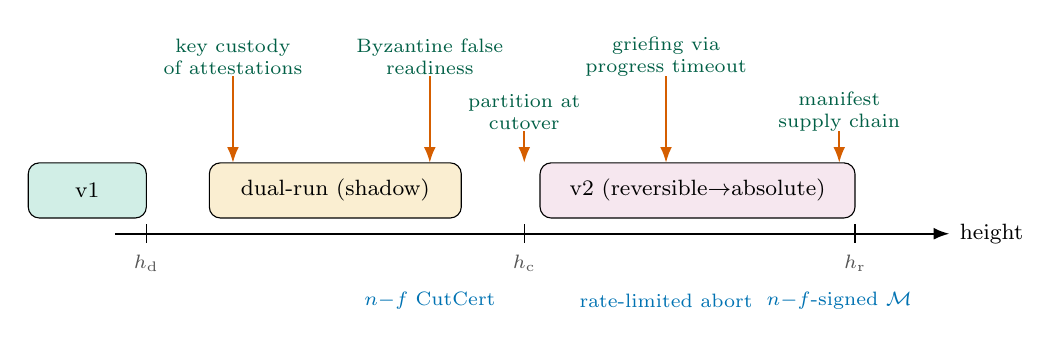
\begin{tikzpicture}[
  font=\footnotesize,
  phase/.style={draw, rounded corners, minimum height=7mm, align=center, fill=#1},
  atk/.style={-{Latex[length=2mm]}, thick, color=cbRed},
  mit/.style={font=\scriptsize, color=cbGreen!60!black, align=center},
  lab/.style={font=\scriptsize, color=cbGray}
]
% timeline axis
\draw[thick,-{Latex[length=2mm]}] (0,0) -- (10.6,0) node[right]{height};
\foreach \x/\t in {0.4/$h_{\mathrm{d}}$, 5.2/$h_{\mathrm{c}}$, 9.4/$h_{\mathrm{r}}$}{
  \draw (\x,0.12) -- (\x,-0.12); \node[lab, below] at (\x,-0.15){\t};
}
% phase bands
\node[phase=cbGreen!18, minimum width=1.5cm] at (-0.35,0.55) {v1};
\node[phase=cbOrange!18, minimum width=3.2cm] at (2.8,0.55) {dual-run (shadow)};
\node[phase=cbPurple!18, minimum width=4.0cm] at (7.4,0.55) {v2 (reversible$\to$absolute)};
% attacks above
\node[mit] at (1.5,2.25) {key custody\\of attestations};
\draw[atk] (1.5,2.0) -- (1.5,0.9);
\node[mit] at (4.0,2.25) {Byzantine false\\readiness};
\draw[atk] (4.0,2.0) -- (4.0,0.9);
\node[mit] at (5.2,1.55) {partition at\\cutover};
\draw[atk] (5.2,1.3) -- (5.2,0.9);
\node[mit] at (7.0,2.25) {griefing via\\progress timeout};
\draw[atk] (7.0,2.0) -- (7.0,0.9);
\node[mit] at (9.2,1.55) {manifest\\supply chain};
\draw[atk] (9.2,1.3) -- (9.2,0.9);
% mitigations below
\node[mit, text=cbBlue] at (4.0,-0.85) {$n{-}f$ CutCert};
\node[mit, text=cbBlue] at (7.0,-0.85) {rate-limited abort};
\node[mit, text=cbBlue] at (9.2,-0.85) {$n{-}f$-signed $\mathcal{M}$};
\end{tikzpicture}}
\caption{Attack surfaces across the migration timeline and their mitigations. Cutover safety
rests on the $n-f$ CutCert (quorum intersection), reversibility on the multi-signed
manifest, and liveness on a rate-limited abort path.}
\label{fig:threat}
\end{figure}

\emph{Partition at cutover.} A partition straddling $h_{\mathrm{c}}$ is the canonical way a
flag-day fork arises: two sides each proceed on their own chain. SAGE neutralizes this because
cutover requires an $n-f$ CutCert, and by quorum intersection (Lemma~\ref{lem:qi}) at most one
partition side can assemble it; the other side keeps the legacy chain and adopts the CutCert
after the partition heals. \emph{Byzantine false readiness.} A Byzantine validator may sign a
readiness attestation for a height at which its local shadow check failed. Because a CutCert
needs $n-f$ signatures and $f<n/3$, every CutCert contains at least $f+1$ correct signers, so
the certified root equals the legacy-finalized root (Theorem~\ref{th:safety}).
\emph{Griefing via the progress timeout.} A Byzantine coalition can stall $\mathcal{C}_2$ to
trip the progress timeout $\tau$ and force a rollback, then repeat. SAGE bounds this by
rate-limiting forced rollbacks to a constant $\rho$ per epoch and by requiring an $n-f$ AbortCert
for a quorum-triggered abort, so $f$ validators cannot by themselves trigger the quorum path. The
key point is that this is a bounded \emph{delay} of migration, not a denial of service to the chain:
the legacy engine $\mathcal{C}_1$ remains the live finalizer until a cutover \emph{succeeds}, so a
stalled target never halts block production---it only postpones the handoff. Proposition~\ref{prop:grief}
bounds the wasted time per epoch. \emph{Manifest supply chain.} A
malicious migration tool could emit a state that is internally consistent but wrong. The
manifest binds the tool hash and is signed by $n{-}f$ validators that independently
recompute the boundary root, so a single compromised tool cannot pass verification; we treat
collusion of $f+1$ key holders as out of scope, consistent with the BFT bound.

\emph{Rollback replay mismatch (operator runbook).} By Corollary~\ref{cor:replay-liveness} a
rollback is always \emph{safe} but is only \emph{clean} (automatic) when the discarded suffix
satisfies Assumption~\ref{as:metadata}. When a suffix transaction violates that precondition, the
deterministic replay onto $\mathcal{C}_1$ produces a divergent root that every correct validator
detects (Lemma~\ref{lem:replay}) rather than committing silently. The prescribed operator response
is then explicit and bounded: (i) the chain has already converged to the legacy-final state
$S_{h_{\mathrm{c}}-1}$, so it is live and safe throughout; (ii) the detected-divergent transactions
are surfaced (not silently dropped) and are re-submitted by their originators against the resumed
legacy chain, exactly as an ordinary un-included transaction would be after any reorg; (iii) no
absolutely-final block is affected, so no client that honored provisional finality observes a
reversion. Thus the only cost of a non-admissible workload is that a fraction of the reversible
window's transactions need re-submission rather than automatic replay---a liveness/convenience
cost, never a safety one.

\begin{table}[t]
\centering
\caption{Abort triggers, the adversary that can invoke each, and the resulting guarantee.}
\label{tab:abort}
\setlength{\tabcolsep}{4pt}
\renewcommand{\arraystretch}{1.2}
\footnotesize
\begin{tabular}{p{0.27\columnwidth}p{0.30\columnwidth}p{0.30\columnwidth}}
\toprule
Trigger & Who can invoke & Guarantee \\
\midrule
Progress timeout $\tau$ & any (incl.\ $f$ Byzantine stalling) & bounded delay $\le\rho(\tau{+}T_{\mathrm{recover}})$/epoch, not denial (Prop.~\ref{prop:grief}) \\
Quorum abort ($n{-}f$) & needs $\ge f{+}1$ correct & cannot be forced by $f$ Byzantine \\
Manifest mismatch & detected locally by any correct node & tamper-evident (Thm.~\ref{th:unforge}) \\
\bottomrule
\end{tabular}
\end{table}

% ===================== PROTOCOL =====================
\section{The SAGE Protocol}
\label{sec:protocol}

SAGE (Shadow-Anchored Graceful Evolution) realizes a heterogeneous engine migration through
four mechanisms: a single-finalizer dual-run invariant, a quorum-certified cutover decision,
an $n{-}f$ multi-signature migration manifest, and a deadline-bounded rollback under a two-tier
finality model. Fig.~\ref{fig:arch} shows the data path, Fig.~\ref{fig:seq} the temporal
message flow, and Fig.~\ref{fig:schedule} the controller as a labeled transition system.

\begin{figure*}[t]
\centering
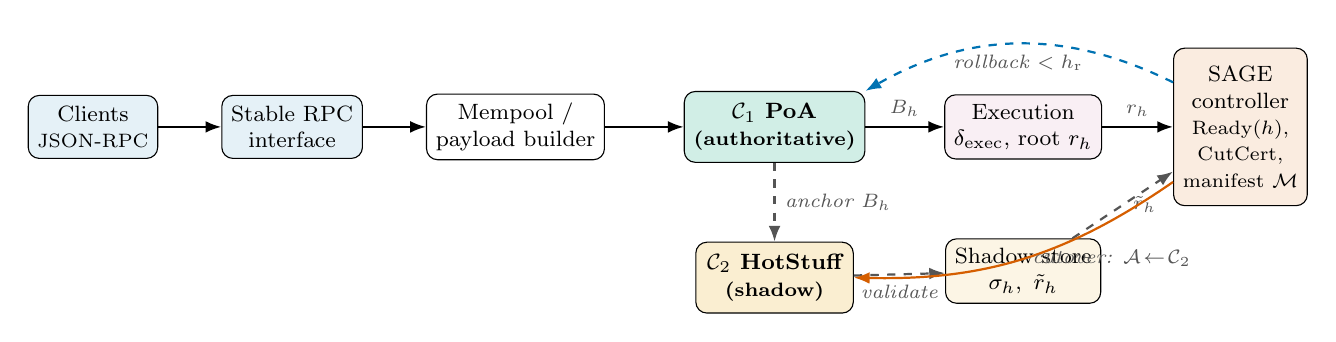
\begin{tikzpicture}[
  node distance=6mm,
  box/.style={draw, rounded corners, align=center, minimum height=8mm, font=\footnotesize, fill=white},
  eng/.style={draw, rounded corners, align=center, minimum height=9mm, minimum width=20mm, font=\footnotesize\bfseries},
  lab/.style={font=\scriptsize\itshape, text=cbGray},
  arr/.style={-{Latex[length=2mm]}, thick},
  darr/.style={-{Latex[length=2mm]}, thick, dashed, color=cbGray}
]
\node[box, fill=cbBlue!10] (client) {Clients\\\scriptsize JSON-RPC};
\node[box, right=8mm of client, fill=cbBlue!10] (rpc) {Stable RPC\\interface};
\node[box, right=8mm of rpc] (pool) {Mempool /\\payload builder};
\node[eng, right=10mm of pool, fill=cbGreen!18] (c1) {$\mathcal{C}_1$ PoA\\\scriptsize (authoritative)};
\node[eng, below=10mm of c1, fill=cbOrange!18] (c2) {$\mathcal{C}_2$ HotStuff\\\scriptsize (shadow)};
\node[box, right=10mm of c1, fill=cbPurple!12] (exec) {Execution\\$\delta_{\mathrm{exec}}$, root $r_h$};
\node[box, below=10mm of exec, fill=cbOrange!10] (shadow) {Shadow store\\$\sigma_h,\ \tilde r_h$};
\node[box, right=9mm of exec, fill=cbRed!12, minimum height=20mm] (ctrl) {SAGE\\controller\\\scriptsize Ready$(h)$,\\\scriptsize CutCert,\\\scriptsize manifest $\mathcal{M}$};
\draw[arr] (client) -- (rpc);
\draw[arr] (rpc) -- (pool);
\draw[arr] (pool) -- (c1);
\draw[arr] (c1) -- node[lab, above]{$B_h$} (exec);
\draw[arr] (exec) -- node[lab, above]{$r_h$} (ctrl);
\draw[darr] (c1) -- node[lab, right]{anchor $B_h$} (c2);
\draw[darr] (c2) -- node[lab, below]{validate} (shadow);
\draw[darr] (shadow) -- node[lab, right]{$\tilde r_h$} (ctrl);
\draw[arr, color=cbRed] (ctrl) to[bend left=18] node[lab, right]{cutover: $\mathcal{A}\!\leftarrow\!\mathcal{C}_2$} (c2.east);
\draw[darr, color=cbBlue] (ctrl) to[bend right=28] node[lab, below]{rollback $<h_{\mathrm{r}}$} (c1.north east);
\end{tikzpicture}
\caption{SAGE data path during dual-run. The legacy engine $\mathcal{C}_1$ is the sole
finalizer and feeds each canonical block $B_h$ to the target engine $\mathcal{C}_2$, which
validates it in shadow mode and records a verdict $\sigma_h$ and a recomputed root
$\tilde r_h$. The controller evaluates the readiness predicate, assembles the CutCert, commits
the multi-signed manifest at cutover, and can transfer authority to $\mathcal{C}_2$ or
roll back to $\mathcal{C}_1$ before the deadline. The client RPC interface is invariant
throughout.}
\label{fig:arch}
\end{figure*}

\begin{figure}[t]
\centering
\resizebox{\columnwidth}{!}{%
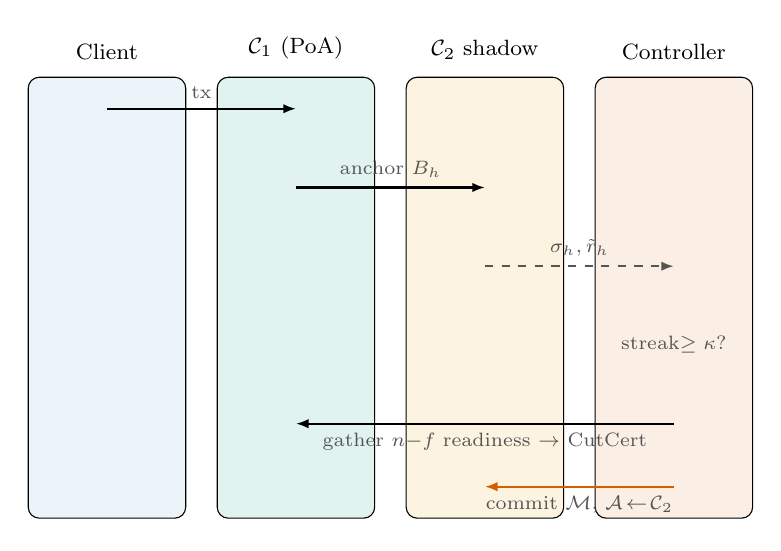
\begin{tikzpicture}[font=\footnotesize,
  lane/.style={draw, rounded corners, fill=#1, minimum width=2.0cm, minimum height=5.6cm, align=center},
  msg/.style={-{Latex[length=1.6mm]}, thick},
  dmsg/.style={-{Latex[length=1.6mm]}, thick, dashed, color=cbGray},
  note/.style={font=\scriptsize, color=cbGray}
]
% lanes
\node[lane=cbBlue!8]  (cl) at (0,0)   {}; \node[above=1mm of cl]{Client};
\node[lane=cbGreen!12](v1) at (2.4,0) {}; \node[above=1mm of v1]{$\mathcal{C}_1$ (PoA)};
\node[lane=cbOrange!12](v2) at (4.8,0){}; \node[above=1mm of v2]{$\mathcal{C}_2$ shadow};
\node[lane=cbRed!10]  (ct) at (7.2,0) {}; \node[above=1mm of ct]{Controller};
% lifelines y positions from top 2.6 down to -2.6
\def\yA{2.4} \def\yB{1.4} \def\yC{0.4} \def\yD{-0.6} \def\yE{-1.6} \def\yF{-2.4}
% tx flow
\draw[msg] (cl.north |- 0,\yA) ++(0,0) -- (v1.north |- 0,\yA);
\node[note, above] at (1.2,\yA){tx};
\draw[msg] (2.4,\yB) -- (4.8,\yB); \node[note,above] at (3.6,\yB){anchor $B_h$};
\draw[dmsg] (4.8,\yC) -- (7.2,\yC); \node[note,above] at (6.0,\yC){$\sigma_h,\tilde r_h$};
\node[note] at (7.2,\yD){streak$\ge\kappa$?};
\draw[msg] (7.2,\yE) -- (2.4,\yE); \node[note,below] at (4.8,\yE){gather $n{-}f$ readiness $\to$ CutCert};
\draw[msg, color=cbRed] (7.2,\yF) -- (4.8,\yF); \node[note,below] at (6.0,\yF){commit $\mathcal{M}$, $\mathcal{A}\!\leftarrow\!\mathcal{C}_2$};
\end{tikzpicture}}
\caption{Temporal message flow for one dual-run cycle and the cutover. The client sees an
unchanged interface; the legacy engine finalizes and anchors each block to the shadow target;
the controller accumulates shadow verdicts, and once the stability streak is reached it
gathers an $n-f$ readiness quorum into a CutCert, commits the multi-signed manifest, and
transfers authority.}
\label{fig:seq}
\end{figure}

\begin{figure}[t]
\centering
\resizebox{\columnwidth}{!}{%
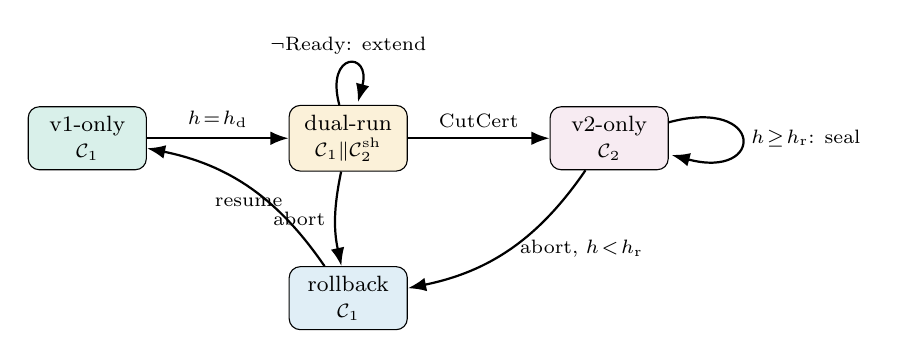
\begin{tikzpicture}[
  >=Latex, node distance=18mm,
  state/.style={draw, rounded corners, minimum width=15mm, minimum height=8mm, align=center, font=\footnotesize, fill=cbBlue!8},
  every edge/.style={draw, ->, thick},
  lab/.style={font=\scriptsize}
]
\node[state, fill=cbGreen!15] (v1) {v1-only\\\scriptsize $\mathcal{C}_1$};
\node[state, right=of v1, fill=cbOrange!15] (dual) {dual-run\\\scriptsize $\mathcal{C}_1\|\mathcal{C}_2^{\mathrm{sh}}$};
\node[state, right=of dual, fill=cbPurple!15] (v2) {v2-only\\\scriptsize $\mathcal{C}_2$};
\node[state, below=12mm of dual, fill=cbBlue!12] (rb) {rollback\\\scriptsize $\mathcal{C}_1$};
\path (v1) edge node[lab, above]{$h\!=\!h_{\mathrm{d}}$} (dual);
\path (dual) edge node[lab, above]{CutCert} (v2);
\path (dual) edge[loop above] node[lab]{$\neg$Ready: extend} (dual);
\path (dual) edge[bend right=12] node[lab, left]{abort} (rb);
\path (v2) edge[bend left=22] node[lab, right]{abort, $h\!<\!h_{\mathrm{r}}$} (rb);
\path (rb) edge[bend right=22] node[lab, below]{resume} (v1);
\path (v2) edge[loop right] node[lab, right]{$h\!\ge\!h_{\mathrm{r}}$: seal} (v2);
\end{tikzpicture}}
\caption{SAGE as a labeled transition system with explicit precedence: abort dominates
cutover at the same height, and dual-run self-loops (extends) while the readiness predicate is
false, so the system is never undefined when stability is not reached by the scheduled height.}
\label{fig:schedule}
\end{figure}

\subsection{Migration Schedule as a Transition System}
A migration is governed by three heights $h_{\mathrm{d}} < h_{\mathrm{c}} \le h_{\mathrm{r}}$
fixed in platform state $P$ and amendable only through the legacy engine before
$h_{\mathrm{d}}$. Rather than a piecewise height function with overlapping cases, we define the
active engine by the labeled transition system of Fig.~\ref{fig:schedule}, with states
$\{\textsc{v1},\textsc{dual},\textsc{v2},\textsc{rollback},\textsc{sealed}\}$ and a fixed
precedence: at any height an enabled abort transition dominates an enabled cutover transition,
and the dual-run state self-loops while the readiness predicate is false. The authoritative
engine $\mathcal{A}(h)$ is $\mathcal{C}_1$ in states \textsc{v1}, \textsc{dual}, and
\textsc{rollback}, and $\mathcal{C}_2$ in \textsc{v2} and \textsc{sealed}. This removes the
ambiguity of an unconditional height-indexed switch: the system has a defined successor in
every state, including the case where stability is not reached by $h_{\mathrm{c}}$, in which
case dual-run is extended.

\subsection{Single-Finalizer Dual-Run}
The central invariant is that at every height exactly one engine finalizes. During
$[h_{\mathrm{d}}, h_{\mathrm{c}})$ the legacy engine $\mathcal{C}_1$ is the sole authority: it
orders and finalizes $B_h$ exactly as before $h_{\mathrm{d}}$. The target engine
$\mathcal{C}_2$ does not propose; it consumes the already-finalized $B_h$, runs its own
validation routine, and records a verdict $\sigma_h$ and the root $\tilde r_h$ it computes for
the same transactions.

\begin{definition}[Shadow mode]
\label{def:shadow}
An engine runs in shadow mode at height $h$ if, for the canonical block $B_h$ finalized by the
authoritative engine, each correct validator runs the shadow engine's validation routine on
$B_h$, records $\sigma_h \in \{\mathsf{valid},\mathsf{invalid}\}$ and $\tilde r_h$ (with
$\tilde r_h=\bot$ if validation rejects), and does not propose or finalize any block. Shadow
validation is a side-effect-free function of $(B_h,S_{h-1})$ and never blocks the finalization
path.
\end{definition}

\subsection{Quorum-Certified Cutover Decision}
Cutover is not a local choice; it is a single agreed decision carried by a certificate.

\begin{definition}[Readiness attestation and CutCert]
\label{def:cutcert}
Governance fixes one boundary tuple
$\beta=\langle\mathrm{cid},e,h_{\mathrm{c}}-1,\mathsf{H}(B_{h_{\mathrm{c}}-1}),r_{h_{\mathrm{c}}-1}\rangle$
before dual-run begins. A correct validator $i$ emits at most one readiness attestation
$\mathsf{att}_i=\mathrm{Sign}_i\langle\textsc{ready},\beta\rangle$ in epoch $e$, and only after its
last $\kappa$ shadow verdicts are valid with matching canonical roots and it has locally finalized
and recomputed the boundary in $\beta$. A CutCert is a set of $n-f$ valid attestations on exactly
that fixed tuple. Validators reject attestations for any other height, parent hash, or root.
Concretely, the artifact realizes an $n-f$ Ed25519 multi-signature: the set of individual EUF-CMA
signatures over the shared tuple, of size $O(n)$. A threshold or BLS aggregate could replace the
list without changing the safety obligation, but its setup and robustness tradeoffs remain future
engineering work.
\end{definition}

\subsection{Threshold-Signed Migration Manifest}
The boundary is bound by a manifest that is cryptographically signed and replay-bound, not a
bare equality check:
\begin{equation}
\mathcal{M} = \big\langle \mathrm{cid}, e, h_{\mathrm{c}}, \mathsf{H}(B_{h_{\mathrm{c}}-1}),
r_{h_{\mathrm{c}}-1}, g_1, g_2, \mathsf{H}_{\mathrm{tool}}, \pi \big\rangle,
\end{equation}
where $g_1,g_2$ are the engine generation identifiers, $\mathsf{H}_{\mathrm{tool}}$ binds the
migration tooling, and $\pi$ is the CutCert over the tuple ($n-f$ signatures in the realized
multi-signature form; see Definition~\ref{def:cutcert}). A
correct validator accepts cutover only if (i) $\pi$ verifies as $n-f$ valid signatures on the tuple,
(ii) the carried root equals the validator's locally recomputed
$\mathrm{root}(S_{h_{\mathrm{c}}-1})$, and (iii) $\mathcal{M}$ is carried in a
$\mathcal{C}_1$-finalized header. The chain identifier and epoch make a manifest from one
migration or chain non-replayable on another.

\subsection{Two-Tier Finality and Bounded Rollback}
To reconcile reversibility with client semantics we adopt two finality tiers. A block is
\emph{absolutely final} if $h < h_{\mathrm{c}}$ (legacy-finalized) or $h \ge h_{\mathrm{r}}$
(sealed target). A block in the reversible window $[h_{\mathrm{c}}, h_{\mathrm{r}})$ is
\emph{provisionally final}: clients are told through an advisory finality flag that it may be
reverted until $h_{\mathrm{r}}$. The abort condition $\textsc{AbortCondition}(h)$ fires when
the target produces no finalized block within the progress timeout $\tau$, when an $n-f$
AbortCert is formed, or when manifest verification fails. On abort before $h_{\mathrm{r}}$ the
controller discards the provisional suffix, resets $\mathcal{A}$ to $\mathcal{C}_1$ at
$S_{h_{\mathrm{c}}-1}$, and resumes legacy finalization; transactions in the discarded suffix
are deterministically replayed onto $\mathcal{C}_1$. After $h_{\mathrm{r}}$ the target is
sealed and rollback is disabled. The advisory flag is the only client-visible change, so a
client that honors provisional finality observes a monotone, uninterrupted chain; this is the
precise sense in which SAGE preserves the client interface. This is the same provisional-versus-
final distinction that GRANDPA~\cite{grandpa} already exposes to clients and that the
``wait-$N$-confirmations'' convention of deployed chains encodes: an integrator that treats a
provisional block as settled does so at its own risk, exactly as it would for an unconfirmed
transaction today, so cross-chain or IBC actions taken on provisional state are the integrator's
documented responsibility rather than a new hazard SAGE introduces.

The claim that the discarded suffix can be \emph{deterministically replayed} onto $\mathcal{C}_1$
holds under an explicit precondition, stated as Assumption~\ref{as:metadata} and proved as
Lemma~\ref{lem:replay}: transaction execution in the reversible window must be a pure function of
the ordered transaction set and parent state, independent of engine-specific block metadata
(timestamp, height, proposer identity) and of external non-deterministic injection (live oracle
reads). In the sovereign/permissioned setting SAGE targets, the operator controls the deployed
contract set and configures the window $[h_{\mathrm{d}}, h_{\mathrm{c}})$, so this precondition is a
checkable deployment constraint rather than a universal assumption; we discuss in
Section~\ref{sec:discussion} that general Turing-complete reversibility with arbitrary oracle
dependence is out of scope and a genuine open problem. Where the precondition does not hold, clean replay is not guaranteed. The controller validates the
manifest-bound replay context and fails closed when that context is missing or mismatched. The implementation additionally binds a \emph{replay context root} into the
rollback anchor: every provisional block in the discarded suffix must carry a matching context
record (chain identifier, height, timestamp, beneficiary, base fee, randomness, and oracle snapshot
root), and rollback is refused if a context is missing, reordered, or does not hash to the manifest
bound root. Thus metadata dependence is not papered over by transaction replay; it is either
explicitly captured or fail-closed. The replay-context record is per provisional block, not per
transaction. In the canonical encoding, a record with an eight-byte chain identifier
occupies $122$ bytes without an oracle root and $162$ bytes with one; in general
the size is $114+|\mathrm{cid}|$ bytes plus an additional $40$ bytes when the optional oracle root
is present, before container or database framing. Even a $1000$-block provisional window is
therefore about $122$--$162$\,KiB per validator for replay context, so the cost is bounded by the
window length rather than by TPS. The prototype keeps these records in the rollback manager's
memory until rollback or the absolute-finality deadline; production nodes can checkpoint them
asynchronously with the normal block metadata, but SAGE does not require synchronous replay-context
disk I/O on the block-validation critical path.

Table~\ref{tab:rollback-compat} makes the workload-dependent behavior concrete by
class, separating the \emph{unconditional} safety guarantee (the chain always returns to the
unique absolutely-final legacy state, or fails closed) from the \emph{conditional} automatic-replay
convenience. The recurring reviewer example, a transaction that reads \texttt{block.timestamp} or
\texttt{block.number}, falls in the third row: it replays cleanly only if its consumed
block-environment values are captured in the replay context, and otherwise surfaces a detected root
mismatch rather than a silent mis-execution.

\begin{table}[t]
\centering
\caption{Rollback behavior by workload class. Safety (return to the unique legacy state or
fail closed) is \emph{unconditional} in every row; only the automatic-replay convenience is
workload-dependent. ``Fail-closed'' means the recomputed root diverges and every correct validator
detects the mismatch (Lemma~\ref{lem:replay}), handing the suffix to operator recovery rather than
committing a wrong state.}
\label{tab:rollback-compat}
\setlength{\tabcolsep}{4pt}
\renewcommand{\arraystretch}{1.2}
\footnotesize
\begin{tabular}{p{0.24\columnwidth}p{0.30\columnwidth}p{0.36\columnwidth}}
\toprule
Workload class & Automatic clean replay? & SAGE behavior \\
\midrule
Metadata-independent (pure transfers, deterministic app logic) & Yes & Deterministic replay reproduces roots; clean, no operator action \\
Block-metadata reads (\texttt{timestamp}, \texttt{number}, \texttt{coinbase}, base fee) & Only if the value is captured in the replay context & With context: clean replay; without: fail-closed detected mismatch \\
Live oracle or external non-determinism & Only if the oracle snapshot root is captured & With snapshot: clean replay; without: fail-closed detected mismatch \\
Cross-chain / IBC actions on provisional state & Not SAGE's to replay & Integrator must await absolute finality ($h\ge h_{\mathrm{r}}$); provisional use is at-risk by the two-tier contract \\
\bottomrule
\end{tabular}
\end{table}

\begin{algorithm}[t]
\caption{SAGE per-height controller at a correct validator}
\label{alg:sage}
\begin{algorithmic}[1]
\Require fixed schedule $(h_{\mathrm{d}},h_{\mathrm{c}},h_{\mathrm{r}})$, threshold $\kappa$, timeout $\tau$
\State $\mathit{state}\gets\textsc{v1}$
\State $\mathit{streak}\gets 0$
\For{each finalized canonical block $B_h$ with root $r_h$}
  \If{$\mathit{state}=\textsc{v1}$ \textbf{and} $h\ge h_{\mathrm{d}}$}\ $\mathit{state}\gets\textsc{dual}$ \EndIf
  \If{\Call{AbortCondition}{$h,\tau$} \textbf{and} $h<h_{\mathrm{r}}$}
     \State retain $\mathcal{A}=\mathcal{C}_1$ or restore it at $S_{h_{\mathrm{c}}-1}$
     \State validate context; replay admissible suffix; $\mathit{state}\gets\textsc{rollback}$; \textbf{continue}
  \EndIf
  \If{$\mathit{state}=\textsc{dual}$}
     \State $(\sigma_h,\tilde r_h)\gets\mathcal{C}_2.\textsc{ShadowValidate}(B_h)$
     \State \textbf{if} $\sigma_h=\mathsf{valid}\wedge\tilde r_h=r_h$ \textbf{then} $\mathit{streak}{+}{+}$ \textbf{else} $\mathit{streak}\gets0$
     \If{$h=h_{\mathrm{c}}-1$ \textbf{and} $\mathit{streak}\ge\kappa$}
        \State broadcast $\mathsf{att}_i$ on fixed boundary tuple $\beta$
        \If{$n-f$ matching attestations form $\mathrm{CutCert}(\beta)$}
           \State commit $\mathcal{M}$ under $\mathcal{C}_1$; initialize $\mathcal{C}_2$ from $r_h$
           \State $\mathcal{A}\gets\mathcal{C}_2$ for $h_{\mathrm{c}}$; $\mathit{state}\gets\textsc{v2}$
        \EndIf
     \EndIf
  \EndIf
  \If{$h\ge h_{\mathrm{r}}$ \textbf{and} $\mathit{state}=\textsc{v2}$}\ seal target; $\mathit{state}\gets\textsc{sealed}$ \EndIf
\EndFor
\end{algorithmic}
\end{algorithm}

\subsection{Design Rationale: Why Each Mechanism Is Necessary}
Each of SAGE's four mechanisms removes a specific failure that the others do not cover, and the
evaluation in Section~\ref{sec:eval} treats these failures as falsifiable invariant checks.
The \emph{single-finalizer dual-run} is what prevents two engines from ever both finalizing;
without it, running two engines in parallel is a latent fork waiting for a partition. The RQ2
exposure metric (Section~\ref{sec:eval}) makes this concrete: under a cutover-straddling
partition with a balanced split, hard fork and blind cutover are exposed to a disjoint-quorum
fork window in $100\%$ of trials while SAGE is exposed in $0\%$. The
\emph{quorum-certified cutover} is what makes the switch a single agreed decision; without it, a
blind schedule lets each partition side switch independently, which is exactly the exposure the
metric records. The \emph{multi-signed manifest} is what makes the boundary
auditable and the rollback verifiable; a bare equality check, as a naive design might use, binds
a value to itself and is forgeable by any proposer, so the unforgeability and replay-resistance
theorems would not hold. The \emph{two-tier finality} is what reconciles reversibility with the
client contract; without an explicit provisional tier, a rollback would revert blocks a client
was told were final, which is a finality reversion and a client-visible safety violation. The
design is therefore minimal in the sense that dropping any one mechanism reintroduces a concrete
failure that the evaluation can produce.

% ===================== ANALYSIS =====================
\section{Theoretical Analysis}
\label{sec:analysis}

We prove decision uniqueness, cross-boundary safety, quantified liveness, migration
termination, rollback correctness, manifest security, the detection bound, and complexity. We
first state the assumptions and the vocabulary the theorems quantify over.

\begin{assumption}[Engine correctness]
\label{as:engines}
Each engine conforms to Definition~\ref{def:engine}. $\mathcal{C}_1$ provides safety under its
authority quorum $\mathsf{Q}_1$, and $\mathcal{C}_2$ provides safety always and liveness after
GST under $\mathsf{Q}_2=2f_2+1$ with $n\ge 3f_2+1$.
\end{assumption}

\begin{assumption}[Deterministic execution]
\label{as:exec}
$\delta_{\mathrm{exec}}$ is deterministic on well-formed blocks, so two correct validators
that apply the same block sequence from the same initial state compute identical roots.
\end{assumption}

\begin{assumption}[Metadata-independent execution in the reversible window]
\label{as:metadata}
For transactions finalized in the reversible window $[h_{\mathrm{c}}, h_{\mathrm{r}})$, execution
is a pure function of the ordered transaction set and the parent state: it does not depend on
engine-specific block metadata (timestamp, height, proposer identity) or on external
non-deterministic inputs (live oracle reads) that could differ between the target attempt and a
legacy replay. In the sovereign/permissioned regime SAGE targets, the operator controls the
deployed contract set and the window length, so this is a checkable deployment constraint.
\end{assumption}

\begin{assumption}[Cryptography]
\label{as:crypto}
$\mathrm{root}(\cdot)$ and $\mathsf{H}$ are collision resistant and the validator signatures are
EUF-CMA secure; the adversary controls at most $f<n/3$ keys.
\end{assumption}

\begin{definition}[Commit and convergence]
\label{def:commit}
$\mathrm{committed}_i(h,B)$ holds if correct validator $i$ has a finalization certificate for
block $B$ at height $h$. Two correct validators \emph{conflict} at $h$ if they commit distinct
blocks. The system \emph{converges} if the committed prefixes of all correct validators are
eventually identical.
\end{definition}

\begin{lemma}[Quorum intersection]
\label{lem:qi}
With $n\ge 3f+1$, any two $(n-f)$-quorums intersect in at least $n-2f\ge f+1$ validators, hence
in at least one correct validator.
\end{lemma}
\begin{proof}
Two sets of size $n-f$ in a universe of size $n$ intersect in at least $2(n-f)-n = n-2f$
elements. With $n\ge 3f+1$, $n-2f\ge f+1$. Since at most $f$ validators are Byzantine, an
intersection of size $\ge f+1$ contains at least one correct validator.
\end{proof}

\begin{lemma}[Safe and live cutover thresholds]
\label{lem:necessity}
Let at most $f$ of $n$ validators be Byzantine and let a boundary certificate require $q$ matching
attestations. Liveness with $f$ silent validators requires $q\le n-f$. To force two certificate
quorums to share a correct validator, safety requires $2q-n>f$, equivalently
$q>(n+f)/2$. Hence every integer threshold in $((n+f)/2,n-f]$ is both safe and live under these
assumptions. SAGE chooses $q=n-f$, the maximal live threshold, maximizing the guaranteed
correct-signer intersection.
\end{lemma}
\begin{proof}
If $q>n-f$, the $n-f$ responsive validators cannot form a certificate. Two size-$q$ sets intersect
in at least $2q-n$ validators; that intersection is guaranteed to contain a correct signer exactly
when $2q-n>f$. A correct validator signs only the fixed epoch boundary tuple, so such an
intersection excludes conflicting certificates. At $q=n-f$, the intersection is at least
$n-2f\ge f+1$ for $n\ge3f+1$. At $n=6,f=1$, both $q=4$ and $q=5$ satisfy the bound; the experiment
contrasts the implemented conservative choice $q=5$ with the unsafe $q=3$ transplant.
\end{proof}

\begin{theorem}[Decision uniqueness]
\label{th:unique}
For a fixed migration epoch $e$, at most one CutCert can certify the governance-fixed boundary
tuple $\beta$. Every correct validator accepting a valid certificate therefore accepts the same
cutover height, parent hash, and boundary root.
\end{theorem}
\begin{proof}
Suppose two valid CutCerts certified conflicting tuples. Their $n-f$ signer sets intersect in at
least $f+1$ validators by Lemma~\ref{lem:qi}, including a correct validator. Definition~\ref{def:cutcert}
permits a correct validator to sign only $\beta$ and at most once in epoch $e$, so it cannot belong
to both conflicting certificates. Signature unforgeability prevents Byzantine validators from
fabricating the missing correct signature.
\end{proof}

\begin{lemma}[Single finalizer during dual-run]
\label{lem:single}
For every height $h\in[h_{\mathrm{d}},h_{\mathrm{c}})$ only $\mathcal{C}_1$ finalizes, and at
most one block is finalized at $h$.
\end{lemma}
\begin{proof}
In state \textsc{dual} the authoritative engine is $\mathcal{C}_1$. By
Definition~\ref{def:shadow} the shadow engine neither proposes nor finalizes; it only validates
the block already finalized by $\mathcal{C}_1$. Finalization at $h$ is therefore governed solely
by $\mathcal{C}_1$, which finalizes at most one block per height (Assumption~\ref{as:engines}).
\end{proof}

\begin{theorem}[Cross-boundary safety]
\label{th:safety}
No two correct validators that follow the SAGE gate conflict at any height, including the fixed
boundary $h_{\mathrm{c}}$.
\end{theorem}
\begin{proof}
Before $h_{\mathrm{d}}$, legacy safety applies. During dual-run, Lemma~\ref{lem:single} gives one
authoritative finalizer. At the boundary, every accepted CutCert names the same legacy-finalized
parent and root by Theorem~\ref{th:unique}; every correct validator recomputes that root before
acceptance. The target is initialized from that certified parent and becomes authoritative only for
height $h_{\mathrm{c}}$ and above. Thus no correct SAGE validator finalizes a legacy block at or above
the target's first authoritative height. Thereafter target-engine safety applies. Induction over
heights yields one canonical committed prefix.
\end{proof}

\begin{theorem}[No scheduled stop on a successful handoff]
\label{th:liveness}
After GST, assuming the legacy engine remains live through dual-run, the fixed CutCert forms within
one bounded communication round once $n-f$ validators are ready. The successful handoff introduces
no explicit stop-the-world phase; its client inter-commit gap is measured empirically. If a
partition prevents the CutCert, SAGE preserves boundary safety by withholding the switch, but this
theorem does not claim that the current prototype continues finalizing through that partition.
\end{theorem}
\begin{proof}
Shadow validation is outside the legacy finalization path. After GST, matching attestations from
$n-f$ responsive validators arrive within one bounded communication round, after which validators
initialize the target from the fixed certified parent and switch at the next height. No snapshot or
scheduled service-stop state occurs. Progress under a cutover-straddling partition depends on the
legacy runtime and is outside this successful-handoff statement.
\end{proof}

\begin{corollary}[Successful-run handoff measurement]
\label{cor:nohalt}
In successful no-partition runs, client-visible interruption is bounded by the measured maximum
inter-commit gap; this is experimental evidence, not a protocol-wide asynchronous liveness bound.
\end{corollary}

\begin{theorem}[Conditional migration completion]
\label{th:termination}
After GST, if the fixed boundary is reached with $n-f$ mutually communicating ready validators, a
CutCert forms within one bounded communication round and migration completes. If a partition
prevents that quorum, migration remains safely pending; completion after healing requires retaining
or retransmitting attestations for the same fixed tuple.
\end{theorem}
\begin{proof}
All correct attestations name the immutable tuple $\beta$. Once $n-f$ ready validators can
communicate, their attestations form the unique CutCert by Theorem~\ref{th:unique}. Before that
condition holds, the gate remains closed and no conflicting switch is authorized.
\end{proof}

\begin{lemma}[Replay equivalence]
\label{lem:replay}
Under Assumptions~\ref{as:exec} and~\ref{as:metadata}, replaying the ordered transactions of the
discarded suffix $[h_{\mathrm{c}}, h_a]$ onto $\mathcal{C}_1$ from state $S_{h_{\mathrm{c}}-1}$
yields the same per-transaction execution outcomes as the target attempt. If Assumption~\ref{as:metadata} fails, equivalence is no longer guaranteed; a missing or
mismatched manifest-bound replay context causes automatic replay to fail closed rather than commit
an unaudited state.
\end{lemma}
\begin{proof}
By Assumption~\ref{as:metadata} each suffix transaction's execution is a pure function of the
ordered transaction set and parent state, with no dependence on block metadata or external
injection; by Assumption~\ref{as:exec} that function is deterministic. Replaying the same ordered
set from the same parent state $S_{h_{\mathrm{c}}-1}$ therefore reproduces identical outcomes and
identical roots. Without Assumption~\ref{as:metadata}, the same outcome may or may not recur, so no converse is
claimed. SAGE instead verifies the captured replay context against the manifest commitment and
refuses automatic replay when that context is missing, reordered, or mismatched.
\end{proof}

\begin{theorem}[Rollback safety]
\label{th:rollback}
If an abort fires at height $h_a<h_{\mathrm{r}}$, every correct validator converges to the
legacy-finalized state $S_{h_{\mathrm{c}}-1}$ with no conflict on absolutely final blocks, and
any tampering with the resumed state is detected. This holds \emph{unconditionally}: it does
not depend on the metadata-independence Assumption~\ref{as:metadata}.
\end{theorem}
\begin{proof}
Blocks in $[h_{\mathrm{c}},h_a]$ are only provisionally final by the two-tier model, so no
absolutely final block is reverted and the client contract on absolute finality is preserved.
The controller retains the $\mathcal{C}_1$ finalization certificate for $S_{h_{\mathrm{c}}-1}$
until $h_{\mathrm{r}}$. On abort it discards the provisional suffix and resets authority to
$\mathcal{C}_1$ at $S_{h_{\mathrm{c}}-1}$. By Theorem~\ref{th:safety} the suffix extended the
unique legacy prefix, so removing it orphans no independently legacy-finalized block.
Convergence to $S_{h_{\mathrm{c}}-1}$ follows from the retained certificate and
Assumption~\ref{as:exec}. If an adversary attempts to resume from $S'\ne S_{h_{\mathrm{c}}-1}$, its root
$r'\ne r_{h_{\mathrm{c}}-1}$ fails manifest acceptance rule (ii) at every correct validator, so
the resume is rejected. By Theorem~\ref{th:unique} the abort decision is unique, so all correct
validators roll back identically. The progress-timeout path is rate-limited to a constant per
epoch, so $f$ Byzantine validators that stall $\mathcal{C}_2$ cannot force unbounded rollbacks.
Crucially, safety here means the chain returns to a single agreed absolutely-final state; it
does \emph{not} assert that the discarded provisional transactions are automatically re-applied,
which is the separate liveness property below.
\end{proof}

\begin{corollary}[Automatic-replay liveness, conditional]
\label{cor:replay-liveness}
If additionally every suffix transaction satisfies Assumption~\ref{as:metadata}
(metadata-independent execution), then the discarded provisional transactions replay
deterministically onto $\mathcal{C}_1$ and reproduce their execution outcomes
(Lemma~\ref{lem:replay}), so the rollback is not merely safe but \emph{clean}: no transaction is
lost and no operator intervention is required. Where Assumption~\ref{as:metadata} fails for some
transaction, the replay produces a divergent root that every correct validator \emph{detects} as
a mismatch (Lemma~\ref{lem:replay}); the system remains safe by Theorem~\ref{th:rollback} but the
affected transactions require operator handling (Section~\ref{sec:threat}) rather than automatic
re-application. Thus safety is unconditional and automatic-replay liveness is exactly as strong as
the workload's admissibility, never weaker on safety.
\end{corollary}
\begin{proof}
The clean-replay case is immediate from Lemma~\ref{lem:replay} under
Assumption~\ref{as:metadata}. For the failing case, the divergent-root detection is the
fail-closed branch of Lemma~\ref{lem:replay}; safety is preserved because the detected mismatch
prevents a wrong state from being committed, and Theorem~\ref{th:rollback} already guarantees
convergence to $S_{h_{\mathrm{c}}-1}$ independent of whether replay succeeds.
\end{proof}

\begin{proposition}[Bounded griefing delay]
\label{prop:grief}
With forced rollbacks rate-limited to $\rho$ per epoch and progress timeout $\tau$, a coalition of
$f$ Byzantine validators that stalls the target engine can waste at most
$\rho\,(\tau + T_{\mathrm{recover}})$ of migration progress per epoch, where $T_{\mathrm{recover}}$
is the cost of resetting authority to $\mathcal{C}_1$ on abort. It cannot deny liveness to the chain.
\end{proposition}
\begin{proof}
Each griefing cycle costs one progress timeout $\tau$ (to detect the stall) plus one rollback
$T_{\mathrm{recover}}$; the rate limit caps such cycles at $\rho$ per epoch, giving the stated bound,
after which further forced rollbacks in the epoch are refused and dual-run simply continues. The
quorum-abort path needs an $n-f$ AbortCert, i.e.\ $\ge f+1$ correct signers, so $f$ Byzantine
validators cannot trigger it. Throughout, $\mathcal{C}_1$ remains the authoritative finalizer
(it is never displaced until a cutover succeeds), so the chain keeps committing blocks at rate
$T_{\mathrm{dual}}$; the attack delays the \emph{migration} by at most $\rho\,(\tau+T_{\mathrm{recover}})$
per epoch but never stalls block production. Hence griefing is a bounded delay, not a liveness denial.
\end{proof}

\begin{theorem}[Manifest unforgeability]
\label{th:unforge}
Under Assumptions~\ref{as:crypto}, an adversary controlling $\le f$ keys cannot produce an
accepted manifest whose committed boundary state differs from the unique legacy-finalized
$S_{h_{\mathrm{c}}-1}$, except with negligible probability.
\end{theorem}
\begin{proof}
An accepted manifest carries a certificate $\pi$ that verifies as $n-f$ signatures
(rule (i)). Suppose an adversary outputs an accepted $\mathcal{M}$ with root
$r'\ne r_{h_{\mathrm{c}}-1}$. Either (a) $\pi$ aggregates a signature from a correct validator on
$r'$, which a correct validator never produces because it signs only its locally recomputed root
(Definition~\ref{def:cutcert}); by Lemma~\ref{lem:qi} an $n-f$ set contains $\ge f+1$ correct
validators, so at least one correct signature on $r'$ is required, contradiction; or (b) the
adversary forged a correct validator's signature, breaking EUF-CMA, which occurs with negligible
probability; or (c) $r'$ collides with $r_{h_{\mathrm{c}}-1}$ under $\mathrm{root}(\cdot)$, which
contradicts collision resistance. Hence acceptance of a wrong-state manifest is negligible.
\end{proof}

\begin{theorem}[Replay resistance]
\label{th:replay}
A manifest valid for $(\mathrm{cid},e)$ does not verify for any $(\mathrm{cid}',e')\ne
(\mathrm{cid},e)$.
\end{theorem}
\begin{proof}
The signed tuple includes $\mathrm{cid}$ and $e$, and attestations are over the same fields
(Definition~\ref{def:cutcert}). Verification recomputes the signed message with the local
$(\mathrm{cid}',e')$; a single differing field changes the message, so $\pi$ fails to verify by
EUF-CMA correctness unless the adversary forges a signature on the new message, which is
negligible.
\end{proof}

\begin{observation}[Shadow detection is coverage-bounded, not detection-rate-bounded]
\label{th:detection}
Shadow validation detects a divergence \emph{deterministically} on any block that exercises the
divergent execution path: by Assumption~\ref{as:exec} the shadow-recomputed root $\tilde r_h$ is a
deterministic function of the block, so a triggered divergence yields $\tilde r_h\ne r_h$ with
certainty (not with some per-block probability $q<1$). Consequently the residual risk of an unsafe
cutover is not a geometric decay in $\kappa$ under an independence assumption; it is governed by
whether the stability window \emph{covers}, i.e.\ actually executes, the divergent path. Let
$p_{\mathrm{div}}$ be the probability a latent divergence exists and $u(\kappa)$ the probability that
none of the $\kappa$ window blocks exercises it under the prevailing workload. Then
$\Pr[\mathrm{unsafe}] = p_{\mathrm{div}}\cdot u(\kappa)$, where $u$ is monotonically non-increasing in
$\kappa$ but workload-dependent and \emph{not} of the form $(1-q)^{\kappa}$: a divergence on a code
path the workload never exercises has $u(\kappa)=1$ for all $\kappa$, while one on a path exercised
every block has $u(1)=0$.
\end{observation}

\begin{remark}
\label{rem:detection-indep}
An earlier formulation modeled per-block detection as independent Bernoulli trials, giving
$p_{\mathrm{div}}(1-q)^{\kappa}$. That model is inappropriate for deterministic state-machine
replication: execution outcomes across blocks are correlated through shared state, not independent,
and a triggered divergence is detected with certainty rather than probability $q$. We therefore state
the residual risk as the coverage bound of Observation~\ref{th:detection} and treat the quantitative
estimation of $u(\kappa)$ for a given workload as an empirical question requiring a latent-divergence
injection campaign (Section~\ref{sec:eval}, RQ3), which we do not claim to resolve here.
\end{remark}

\begin{theorem}[Message and round complexity]
\label{th:complexity}
Dual-run adds zero wire messages per block. Cutover costs $O(n)$ messages per collector (or
$O(n^2)$ all-to-all) and $O(1)$ extra rounds; abort costs the same. Steady-state per-engine
complexity is unchanged.
\end{theorem}
\begin{proof}
Shadow validation is local (Definition~\ref{def:shadow}), adding no messages. Forming a CutCert
gathers $n-f=O(n)$ attestations, $O(n)$ at a designated collector or $O(n^2)$ broadcast, in one
round; verification is $O(n)$ work but $O(1)$ rounds. The certificate itself is $O(n)$ in size in the
multi-signature form the artifact uses; replacing it with a threshold/BLS aggregate would change the
constant factors and key-management assumptions but not the quorum-intersection proof. The AbortCert
is symmetric. Outside the one-time decision, each engine runs unchanged, so steady-state
complexity is preserved.
\end{proof}

\begin{proposition}[Boundary latency]
\label{prop:bdy}
After GST, the gap between the last legacy commit and the first target commit is at most
$T_{\mathrm{bdy}} = \Delta_{\mathrm{cert}} + T_{\mathrm{init}} + (k{+}1)\,2\Delta$, where
$\Delta_{\mathrm{cert}}$ is the one-round CutCert gather, $T_{\mathrm{init}}$ is the target
first-view setup, and $k\le f$ is the number of faulty target leaders before an honest one,
each adding one pacemaker timeout round; with an honest first leader ($k{=}0$) this reduces to
$\Delta_{\mathrm{cert}} + T_{\mathrm{init}} + 2\Delta$.
\end{proposition}
\begin{proof}
The CutCert gathers $n-f$ attestations in one post-GST round, so it forms within
$\Delta_{\mathrm{cert}}\le\Delta$ plus $O(n)$ local verification. The target then runs
$\mathsf{Init}$ in $T_{\mathrm{init}}$. Each faulty target leader forfeits its view after one
pacemaker timeout of $O(\Delta)$; at most $k\le f$ such views precede an honest leader, after
which responsiveness completes a quorum certificate within $2\Delta$. Summing gives the bound;
every term is finite after GST, and the legacy engine finalizes throughout the target's view
changes, so the handoff cannot stall block production.
\end{proof}

\subsection{Overhead Analysis}
Before $h_{\mathrm{d}}$ and after $h_{\mathrm{c}}$ SAGE adds no work to the finalization path.
During dual-run each correct validator performs one shadow validation per block, costing
$O(|B_h|)$ re-execution plus an $O(1)$ root comparison; since this is off the critical path the
measured throughput overhead is small and roughly constant in $n$ (Section~\ref{sec:eval}).
Cutover is a one-time $O(n)$ attestation gather plus multi-signature verification, and rollback is an
$O(1)$ authority reset plus an $O(1)$ manifest check. Space is $O(\kappa)$ for the verdict window
plus one retained certificate and at most $h_{\mathrm{r}}-h_{\mathrm{c}}$ provisional blocks.

To confirm that the $O(n)$ certificate is cheap in absolute terms rather than merely
asymptotically bounded, Table~\ref{tab:certtiming} reports the \emph{measured} cost of
producing and verifying a real $n{-}f$ Ed25519 multi-signature over the swept validator count.
Even at $n{=}200$ (an $n{-}f{=}134$-signature certificate) the full certificate verifies in
about $4.5\,$ms at the median and occupies under $10\,$KiB. Because the certificate is formed and
verified exactly once per migration boundary---not per block---this is a negligible fraction of
the empirical boundary-to-boundary cadence (Section~\ref{sec:eval}), so the $O(n)$ multi-signature
is a practical choice and constant-size aggregation is an optimization rather than a necessity.
The signing figure is the summed cost across all $n{-}f$ signers; the gather term is a modeled
one-round-trip cost, not a live-network measurement (real gather latency is reported in the
multi-process and real-host tiers).

\begin{table}[t]
\centering
\caption{Measured CutCert cost with real Ed25519 signatures (the artifact's \texttt{real-crypto}
scheme). ``Sign (all)'' is the summed wall time to produce all $n{-}f$ signatures; ``Verify
p50/p95'' is the wall time to verify the whole $n{-}f$-signature certificate, over $1000$
iterations; ``Cert size'' is the serialized multi-signature. The one-shot boundary cost is small
in absolute terms even at $n{=}200$, so the $O(n)$ certificate needs no aggregation to be
practical. The gather term is modeled (one round-trip), not measured, and is omitted here.}
\label{tab:certtiming}
\setlength{\tabcolsep}{5pt}
\renewcommand{\arraystretch}{1.2}
\footnotesize
\resizebox{\columnwidth}{!}{%
\begin{tabular}{ccccc}
\toprule
$n$ & $n{-}f$ signers & Sign (all, $\mu$s) & \makecell{Verify p50 / p95 ($\mu$s)} & Cert size (B) \\
\midrule
$31$  & $21$  & $311$  & $695$ / $726$   & $1512$ \\
$64$  & $43$  & $722$  & $1440$ / $1494$ & $3096$ \\
$100$ & $67$  & $1132$ & $2236$ / $2453$ & $4824$ \\
$200$ & $134$ & $2187$ & $4482$ / $4924$ & $9648$ \\
\bottomrule
\end{tabular}%
}
\end{table}

% ===================== EVALUATION =====================
\section{Experimental Evaluation}
\label{sec:eval}

\subsection{Methodology}
We evaluate SAGE along three complementary evidence tiers. The first is a
deterministic event-driven simulator in which $n$ validators exchange delayed messages and
finalize blocks under explicit quorum rules; it provides breadth (seed sweeps, parameter
ablations) and a deterministic, replayable safety invariant. The second is a multi-process
testbed in which validators run as separate operating-system processes communicating over
loopback TCP, which realizes the concurrent two-leader execution the serialized simulator cannot
and therefore exhibits observed cross-boundary forks. The third is a bounded TLA+/TLC model check
that exhaustively explores the controller's state space. The implemented simulator safety metric
is an executable invariant over committed logs: two correct validators committing conflicting
blocks at the same height would be reported as a violation. We compare
four migration strategies, stop-the-world (STW), an uncoordinated hard fork (HF),
reconfiguration only (RC), and SAGE, plus an ablation SAGE-BLIND that cuts over on schedule
without a CutCert. The recorded metrics include finalized blocks, downtime blocks,
finality gap, cutover-evidence latency, migration success, rollback occurrence and latency,
absolute-reversion refusal, observed safety violations, and the disjoint-quorum exposure count.
We additionally compare against a Cox-style live homogeneous switch (Section~\ref{sec:related}),
the closest live-switch comparison class. Every strategy in a given experiment is run under an
\emph{identical} configuration---the same $n$, $f$, transaction load, seeds, network-delay model,
pacemaker/view timeout, warm-up, and measurement window---so that the comparison is a fair
same-conditions measurement. Table~\ref{tab:fairness} makes this ``both runners run exactly the
same course'' guarantee explicit: it lists every knob and the single shared value each strategy
receives, and the guarantee is enforced in code, not merely asserted---each experiment binary
clones one \texttt{SimConfig} and mutates only \texttt{StrategyKind} per arm, so no per-arm knob
override is even reachable. The \emph{only} independent variable across arms is the migration
strategy itself.

\begin{table*}[t]
\centering
\caption{Fairness contract for the multi-arm comparisons: every knob is held at a single shared
value across \emph{all} strategy arms (SAGE, Cox-style, Cox-threshold, hard fork, stop-the-world,
reconfiguration). Within a paired campaign, each binary clones one \texttt{SimConfig} and overrides only the strategy. Separate campaigns use the experiment-specific values listed below. ``RQ1/cost'' is the migration-cost + throughput experiment;
``RQ2/safety'' is the partition testbed.}
\label{tab:fairness}
\setlength{\tabcolsep}{5pt}
\renewcommand{\arraystretch}{1.15}
\footnotesize
\begin{tabular}{p{0.42\textwidth}p{0.24\textwidth}p{0.24\textwidth}}
\toprule
Knob (shared within campaign) & RQ1/cost & RQ2/safety \\
\midrule
Validators $n$                & $20$          & $6$ \\
Fault bound $f$               & $6$           & $1$ (BFT quorum $3$) \\
Max height                    & $40$          & $8$ \\
Migration schedule $(h_d,h_c,h_r)$ & $(10,30,40)$ & $(2,4,8)$ \\
Mean message delay            & $40\,\mu$s    & real TCP \\
Stability threshold $\kappa$  & $8$           & $1$ \\
Partition                     & none          & $3/3$ at $h_c$ \\
Seeds / trials per arm        & $60$          & $10$--$20$ \\
Hardware / harness            & one host, one process & one host, real sockets \\
RNG                           & seeded, deterministic & seeded, deterministic \\
\midrule
\textbf{Paired variable} & \multicolumn{2}{c}{\texttt{StrategyKind}} \\
\bottomrule
\end{tabular}
\end{table*}
RQ1 uses $60$ seeds per strategy, RQ2 uses $30$ seeds per partition cell ($180$ rows per strategy
over three split sizes and two durations), RQ3 uses $20$ seeds per $\kappa$, RQ4 uses $20$ seeds
per abort height, and the serialized simulator safety campaign uses $200$ trials per strategy. The scaling
sweep covers $n\in\{4,7,10,13,16,20,25,31,50,100\}$ and the sensitivity sweep covers mean message delays
$\{20,40,80,160,320,640\}\,$ms, each with $20$ trials per point. Table~\ref{tab:rqmap} maps research
questions to experiments.

\begin{table*}[t]
\centering
\caption{Claim-scope map: for each SAGE property, the strongest form of evidence we
provide and its scope. ``Proved'' = pen-and-paper theorem; ``TLC'' = exhaustive bounded
model check ($n\in\{4,7,10\}$); ``Sim'' = deterministic simulator campaign; ``Real host''
= multi-process run on independent cloud VMs; ``Future'' = explicitly not yet established.
The table is deliberately conservative: where a property is only model-checked at small
$n$ or only simulated, we say so rather than implying a general guarantee.}
\label{tab:claimscope}
\setlength{\tabcolsep}{4pt}
\renewcommand{\arraystretch}{1.15}
\footnotesize
\begin{tabular}{p{0.48\textwidth}ccccc}
\toprule
Property & Proved & TLC & Sim & \makecell{Real\\host} & Future \\
\midrule
Cross-boundary safety (Thm~\ref{th:safety})        & \checkmark & \checkmark & \checkmark & \checkmark & \\
Decision uniqueness (Thm~\ref{th:unique})          & \checkmark & \checkmark & \checkmark &            & \\
No absolute reversion (Thm~\ref{th:rollback})      & \checkmark & \checkmark & \checkmark &            & \\
Observed fork differential                          &            &            &            & \checkmark & \\
No scheduled stop, successful handoff (Thm~\ref{th:liveness}) & \checkmark &            & \checkmark & \checkmark & \\
Rollback safety (fail-closed)                       & \checkmark & \checkmark & \checkmark &            & \\
Automatic-replay liveness (Assum.~\ref{as:metadata})& \checkmark &            & \checkmark &            & \\
Cutover cost $O(n)$ msgs / $O(1)$ rounds            & \checkmark &            & \checkmark &            & \\
Throughput parity vs Cox-style comparison class                 &            &            & \checkmark &            & \\
Safety at $n$ in the hundreds                       & \checkmark &            & \checkmark &     & \\
Finality-latency distribution ($p_{50/95/99}$)      &            &            &            & \checkmark & \\
Geo-distributed (cross-region) throughput           &            &            &            &            & \checkmark \\
Cox-threshold head-to-head (20 trials/arm)          &            &            & \checkmark &            & \\
Mechanized proof over all $n$                       &            &            &            &            & \checkmark \\
\bottomrule
\end{tabular}
The $n{=}100$ entry is a SAGE-only simulator robustness sweep ($20$ trials/point), not a
multi-arm or real-host comparison.
\end{table*}

\emph{What each tier proves, and what it does not.} We state the scope of each tier up front to
avoid conflating their evidence. The simulator provides \emph{breadth and reproducibility}: many
seeds, parameter sweeps, and a deterministic, replayable safety invariant; it \emph{cannot} realize
a concurrent two-leader fork, because it serializes one proposer per height, so a $0\%$ observed-fork
rate in the simulator is a property of the model, not evidence of safety, and we never present it as
such. The multi-process testbed provides \emph{realism of the safety claim}: real operating-system
processes, real signatures, a genuine transport-level partition, and active Byzantine equivocation,
so a fork can actually occur and is detected when it does; this tier is the headline safety evidence.
The multi-process testbed has two sub-tiers: a single-machine loopback deployment that supplies the
statistically repeated differential ($0/20$ vs $20/20$), and a real multi-host deployment on six
independent cloud VMs (one validator per host, real TCP) that reproduces the same differential
($0/5$ vs $5/5$, Table~\ref{tab:multihost}) with independent kernels, clocks, and network stacks,
removing the co-location objection for the safety claim. The real multi-host arm was additionally
repeated under an injected $\approx 104$\,ms inter-VM RTT (\texttt{tc netem}), and the differential
held ($0/3$ vs $3/3$), so the gate is not an artifact of near-zero same-region latency. Neither
sub-tier measures geo-distributed \emph{throughput} or finality-latency \emph{distributions}, which
remain future work.
The bounded model check provides \emph{exhaustive correctness at small $n$}: every reachable
controller state under all partition splits for $n\in\{4,7,10\}$. It abstracts deterministic replay
as a guarded predicate and does not model the byte-level replay-context-root hash; the concrete
hash binding and fail-closed replay-context checks are covered by the Rust controller tests. The
simulator's microsecond latencies are \emph{evidence-processing costs in simulator time}, not
wall-clock deployment latency. The netem-impaired loopback tier adds loss, delay, and jitter on
real sockets, but it remains a single-machine bridge tier rather than a geo-distributed WAN
deployment or an absolute TPS benchmark. The four netem profiles are representative engineering
buckets, not measurements from a specific provider: delay is configured as one-way delay, so the
approximate RTT is twice the listed delay before queuing and scheduler noise; jitter and loss are
chosen to bracket common same-region, continental, global, and adverse WAN conditions. The exact
profiles are metro $(10\,\mathrm{ms},2\,\mathrm{ms},0\%)$, continental
$(50\,\mathrm{ms},10\,\mathrm{ms},0.1\%)$, intercontinental
$(120\,\mathrm{ms},25\,\mathrm{ms},0.5\%)$, and adverse
$(200\,\mathrm{ms},50\,\mathrm{ms},1\%)$, listed as one-way delay, jitter, and packet loss.
Determinism buys reproducibility of the protocol-logic results; the loopback-impaired tier buys
additional network realism; neither substitutes for multi-host throughput and finality
measurements.

\begin{table}[t]
\centering
\caption{Mapping of research questions to experiments.}
\label{tab:rqmap}
\renewcommand{\arraystretch}{1.12}
\footnotesize
\begin{tabular}{p{0.72\columnwidth}c}
\toprule
Research question & Exp. \\
\midrule
RQ1: migration cost vs.\ baselines (downtime, gap, overhead, cutover) & E1 \\
RQ2: does SAGE prevent the forks that HF and blind cutover admit? & E5 \\
RQ3: contribution of shadow anchoring and $\kappa$ to safe cutover & E2 \\
RQ4: rollback correctness and scaling with $n$ & E3,E4 \\
\bottomrule
\end{tabular}
\end{table}

\subsection{RQ1: Migration Cost}
Table~\ref{tab:main} reports the deterministic RQ1
configuration ($n=20$, $f=6$, $40$ simulated heights, $60$ seeds, $\kappa=8$). The experiment is
a protocol-functional comparison rather than an absolute throughput benchmark: simulator time is
event based and the workload uses $16$ synthetic accounts. The key point is that each baseline
fails on a \emph{different} axis, so no single scalar ranks them; we therefore report the axis on
which each is designed to fail. Stop-the-world halts finalization during its snapshot/restart
window, and this interruption is \emph{observed} from the recorded finalization timestamps as the
largest gap between consecutive heights---it is not derived from the strategy label. With an
$8\,$ms modeled snapshot/restart cost, stop-the-world exhibits a mean observed downtime of
$8.11\,$ms versus $0.12\,$ms for the no-scheduled-stop strategies, a near two-order-of-magnitude
separation. Hard fork incurs \emph{no} downtime (its failure axis is fork exposure, RQ2), and
reconfig-only is the BFT-SMaRt-style membership-reconfiguration analogue: it changes the
validator view within the same consensus protocol but never actually replaces the consensus
engine, so its $\approx 0.12\,$ms downtime is indistinguishable from SAGE in magnitude while
failing the engine-migration objective. SAGE
finalizes the full workload with no halt and records a mean cutover-evidence latency of
$105.6\,\mu$s. The artifact also includes a matched local microbenchmark
that sweeps transaction load for \emph{three} arms run under
\emph{identical} configuration---a baseline PoA/reconfiguration path, SAGE dual-run, and a
Cox-style live homogeneous switch---recording committed TPS, process CPU, and RSS over five seeds per
load point. Our comparison arm is a \emph{Cox-inspired control modeled on our own engine interface},
not an execution of Cox's implementation (no public Cox artifact was located; see
Section~\ref{sec:related}); we adopt Cox as the reference \emph{design} because it is the closest recent
peer-reviewed protocol we identified for this problem class: Cox~\cite{cox} (\emph{Blockchain: Research
and Applications}, 2026) is the most recent peer-reviewed protocol for zero-downtime \emph{runtime
switching of the consensus engine}, which is precisely SAGE's objective, so it---not a generic
reconfiguration or hard-fork scheme---is the reference point a fair evaluation must clear. Because all three arms use the same seeds, transaction load, validator count,
threshold, and measurement window, the comparison is a fair same-conditions measurement rather
than a cross-configuration one (the exact shared knobs are enumerated in the reproducibility
appendix). Absolute wall-clock TPS is simulator-capacity- and machine-dependent, so the invariant
we report is the \emph{relative} spread across arms. On this CPU-bound local benchmark the three
arms have similar observed means: across all load points SAGE stays within $-2.5$ to
$+2.8\%$ of the Cox-style arm and within $+1.6$ to $+13.5\%$ of the reconfiguration baseline, with
no consistent penalty direction, while CPU stays within $\pm4\%$ and RSS within a fraction of a
MiB. Table~\ref{tab:overhead} reports representative rows. We therefore use the table only as
evidence that shadow validation imposes no large local compute or memory cost and that SAGE's
throughput is on par with the Cox-style comparison class under identical conditions---not as a production
throughput claim. WAN-latency socket behavior is evaluated separately under a controlled netem
round-trip time on real independent hosts (Section~\ref{sec:discussion}, Table~\ref{tab:wanhost}).

\begin{table}[t]
\centering
\caption{Three-arm dual-run overhead microbenchmark; mean over
five seeds per load point, all arms run under identical configuration. Throughput is normalized to
the reconfiguration baseline ($=100\%$) because absolute wall-clock TPS is machine-dependent; the
scientifically stable quantity is the relative spread. SAGE and the Cox-style comparison arm have similar observed means (SAGE within $-2.5$ to $+2.8\%$ of Cox-style across all load
points), showing similar cost in these trials and separate only on
adversarial boundary safety (RQ2), not throughput.}
\label{tab:overhead}
\setlength{\tabcolsep}{5pt}
\footnotesize
\begin{tabular}{rrrrr}
\toprule
Tx/block & \makecell{Baseline\\(norm.)} & \makecell{SAGE\\(rel.\ base)} & \makecell{Cox-style\\(rel.\ base)} & \makecell{SAGE vs\\Cox-style} \\
\midrule
10  & $100\%$ & $+8.5\%$  & $+9.2\%$  & $-0.6\%$ \\
25  & $100\%$ & $+13.5\%$ & $+10.4\%$ & $+2.8\%$ \\
50  & $100\%$ & $+8.7\%$  & $+9.2\%$  & $-0.4\%$ \\
100 & $100\%$ & $+6.3\%$  & $+8.5\%$  & $-2.0\%$ \\
250 & $100\%$ & $+8.4\%$  & $+8.7\%$  & $-0.3\%$ \\
500 & $100\%$ & $+1.6\%$  & $+4.1\%$  & $-2.5\%$ \\
\bottomrule
\end{tabular}
\end{table}

We test the downtime contrast statistically. For each baseline we compare its per-seed observed
downtime against SAGE's using the two-sided Mann--Whitney $U$ test (no normality assumption),
report the rank-biserial effect size, and control the family-wise error rate across the four
comparisons with Holm--Bonferroni at $\alpha=0.05$. SAGE versus stop-the-world is significant
with a maximal effect ($p\approx 2.9\times10^{-11}$, rank-biserial $=+1.0$, Holm-adjusted
$\alpha=0.0125$, reject). SAGE versus hard fork is not significant ($p=1.0$, effect $0$), which
is correct: both preserve service during the migration decision and their separation lives in RQ2, not here. SAGE versus the
Cox-inspired live switch is likewise not significant ($p=1.0$, effect $0$, means $122.6\,\mu$s
each): the closest live-switch comparison class ties SAGE on cost, so our comparison credits Cox's
zero-downtime strength while avoiding a claim to reimplement Cox's full recovery protocol; the
SAGE advantage is isolated to adversarial boundary safety, not migration cost. SAGE versus
reconfig-only is significant by $p$-value ($p\approx 8.9\times10^{-6}$) but the absolute
difference is only $\approx 6\,\mu$s; we flag this as a case where statistical significance does
not imply practical significance, and reconfig-only's substantive failure is the absence of a
protocol swap, not downtime. The complete per-comparison statistics are reported in
Table~\ref{tab:main}.

\begin{table}[t]
\centering
\begin{threeparttable}
\caption{Migration cost against baselines at $n=20$, $f=6$, $40$ heights,
$16$ accounts, $\kappa=8$, mean over $60$ seeds. Downtime is the observed largest gap
between consecutive finalization timestamps (modeled stop-the-world snapshot/restart cost
$8\,$ms). ``Swap'' is whether the consensus engine is actually replaced. Each baseline is
designed to fail on a different axis, so no single column ranks them. Adversarial safety is
\emph{not} evaluated here (the serialized simulator cannot fork by construction); it is
reported in Table~\ref{tab:testbed}.}
\label{tab:main}
\setlength{\tabcolsep}{4pt}
\renewcommand{\arraystretch}{1.2}
\footnotesize
\begin{tabular}{lcccc}
\toprule
Strategy & \makecell{Finalized\\blocks} & \makecell{Downtime\\(ms)} & \makecell{Cutover\\latency ($\mu$s)} & \makecell{Engine\\swap} \\
\midrule
SAGE            & 800 & 0.12 & 105.6          & \checkmark \\
Stop-the-world  & 800 & 8.11 & ---\tnote{a}   & \checkmark \\
Hard-fork       & 800 & 0.12 & ---\tnote{a}   & \checkmark \\
Reconfig-only   & 800 & 0.12 & ---\tnote{a,b} & \texttimes \\
Cox-inspired\tnote{c} & 800 & 0.12 & ---\tnote{a}   & \checkmark \\
\bottomrule
\end{tabular}
\begin{tablenotes}\footnotesize
\item[a] No certified-cutover phase: only SAGE gathers $n{-}f$ cutover evidence, so cutover
latency is undefined for the other strategies (not zero).
\item[b] Reconfiguration-only models a BFT-SMaRt-style dynamic reconfiguration~\cite{bftsmart}:
membership/view change within one engine and one fault model. It is an analogue, not a
reimplementation of the BFT-SMaRt Java library, and it has no engine swap.
\item[c] A Cox-inspired~\cite{cox} live switch modeled on our engine interface: a zero-downtime
switch on a quorum-certified boundary checkpoint analogous to Cox's \emph{StableCheckpoint},
applied across the heterogeneous PoA$\rightarrow$BFT boundary. This is \emph{not} a Cox-threshold
reimplementation (it omits the epoch-mismatch catch-up sub-protocol), so the table evaluates the
checkpoint-switch design axis rather than Cox itself. On the cost axis it is statistically
indistinguishable from SAGE---mean observed downtime $122.6\,\mu$s for both, two-sided
Mann--Whitney $U$ $p=1.0$, rank-biserial $0$, Holm-adjusted $\alpha=0.05$, fail to reject---so the
comparison credits Cox's zero-downtime strength rather than constructing a straw man. The two
strategies separate not on cost but on adversarial boundary safety (RQ2): the Cox-inspired baseline
lacks SAGE's $n{-}f$ dual-run cutover gate.
\end{tablenotes}
\end{threeparttable}
\end{table}

\subsection{RQ2: Adversarial Safety (Falsifiable)}
The central correctness claim remains falsifiable: a partitioned run that produces conflicting
commits would violate the executable safety invariant. We report two distinct quantities and are
careful not to conflate them. The first is the \emph{observed} fork rate: the fraction of trials
in which two distinct blocks finalize at the same height (the executable invariant). The second
is the \emph{disjoint-quorum exposure rate}: the fraction of trials in which a non-CutCert
cutover leaves both partition sides simultaneously holding $\ge$ BFT quorum ($2f{+}1$), so that
the target engine \emph{could} finalize conflicting blocks on each side. Exposure is a structural
precondition for a flag-day fork; an observed fork is its realization.

The simulator exposure matrix uses $n{=}10$, $f{=}2$ (BFT quorum $5$), three split sizes
$\{2,3,5\}$, two partition durations, and fifteen seeds per cell; the partition begins exactly at
the cutover height $h_{\mathrm{c}}$. Under this design the disjoint-quorum metric cleanly
separates the strategies. At the balanced split ($5/5$, the only split where both sides reach
quorum~$5$), hard fork and blind cutover are exposed in $100\%$ of trials, while SAGE is exposed
in $0\%$: its CutCert gate prevents either isolated side from switching engines, so no exposure
window ever opens. At unbalanced splits ($2$ or $3$) no side reaches quorum and exposure is $0\%$
for all strategies, matching the $n\ge 4f{+}2$ feasibility bound. This is the quorum-intersection
argument made empirical: SAGE is the only strategy that eliminates the fork-exposure window under
a cutover-straddling partition.

Exposure is a necessary condition, not a realized fork. The simulator deliberately serializes
finalization through a single proposer per height to keep runs reproducible, so it never drives
two leaders concurrently and the observed fork rate is identically zero for every strategy,
including the exposed blind cells. We therefore do not draw the central safety conclusion from the
simulator; we draw it from the multi-process testbed below, where two leaders genuinely run at
once and a fork can actually occur.

\begin{figure}[t]
\centering
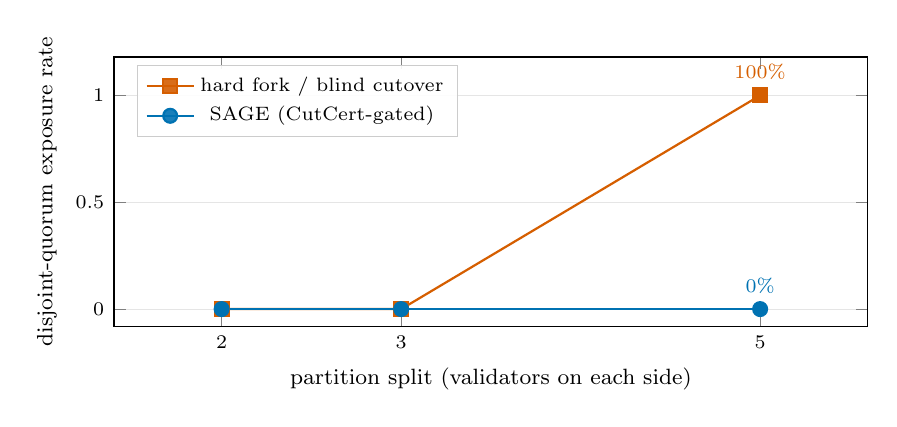
\begin{tikzpicture}
\begin{axis}[
  width=0.92\columnwidth, height=5.0cm,
  tick label style={font=\scriptsize}, label style={font=\footnotesize},
  xlabel={partition split (validators on each side)},
  ylabel={disjoint-quorum exposure rate},
  xmin=1.4, xmax=5.6, ymin=-0.08, ymax=1.18,
  xtick={2,3,5}, ytick={0,0.5,1.0},
  ymajorgrids, grid style={gray!20},
  legend style={at={(0.03,0.97)}, anchor=north west, font=\scriptsize,
    draw=gray!40, fill=white, fill opacity=0.9, text opacity=1},
  nodes near coords, point meta=explicit symbolic,
  every node near coord/.style={font=\scriptsize, yshift=2pt},
]
\addplot[color=cbRed, mark=square*, thick, mark size=2.5pt] coordinates {
  (2,0)[] (3,0)[] (5,1)[$100\%$]};
\addlegendentry{hard fork / blind cutover}
\addplot[color=cbBlue, mark=*, thick, mark size=2.5pt] coordinates {
  (2,0)[] (3,0)[] (5,0)[$0\%$]};
\addlegendentry{SAGE (CutCert-gated)}
\end{axis}
\end{tikzpicture}
\caption{Disjoint-quorum exposure in the simulator ($n{=}10$, $f{=}2$, BFT quorum $5$,
$15$ seeds per cell, partition at $h_{\mathrm{c}}$). Exposure---both partition sides
simultaneously holding BFT quorum, the structural precondition for a fork---appears only at the
balanced $5/5$ split, the sole split where $n\ge 4f{+}2$ admits two independent quorums. There,
hard fork and blind cutover are exposed in every trial ($100\%$), while SAGE's CutCert gate keeps
either isolated side from switching engines, so its exposure stays at $0\%$ at every split.
Exposure is a necessary precondition for a fork, not a realized fork; the realized fork contrast
is reported in Table~\ref{tab:testbed}.}
\label{fig:safety}
\end{figure}

\paragraph{Observed forks in the multi-process testbed.}
Because the simulator cannot realize a concurrent two-leader conflict, the central safety claim
is evaluated in a multi-process testbed in which $n{=}6$ validators ($f{=}1$, BFT quorum
$2f{+}1{=}3$) run as separate operating-system processes that communicate over loopback TCP, sign
the cutover certificate with real Ed25519 keys, and are subjected to a transport-level partition
into two isolated groups of three at the cutover height. Each group can then reach its own quorum
of three concurrently, so two leaders run at once, which is exactly the precondition a serialized
model elides. An executable fork detector inspects the committed logs of all six processes and
reports a fork whenever two distinct blocks are finalized at the same height. Table~\ref{tab:testbed}
gives the result. The blind hard-fork control forks in
every run ($20/20$): both groups switch engines at the scheduled height and finalize conflicting
blocks. A Cox-inspired live switch---modeled on our engine interface with a quorum-certified
boundary checkpoint but \emph{without} SAGE's $n{-}f$ dual-run cutover gate---also forks in every
run ($10/10$). Quorum-gated SAGE forks in none ($0/20$): neither isolated group of three reaches
the $n{-}f{=}5$ cutover quorum, so no side switches engines and the legacy finalizer remains
unique. All three arms share the same process testbed, real Ed25519 signatures, TCP transport,
partition schedule, fork detector, and HotStuff target implementation---including the same
pacemaker and double-vote-tolerant message handler---and differ only in whether the $n{-}f$
cutover quorum gate is enforced. Because both the blind control and the Cox-inspired switch fork
in every run while SAGE never does, SAGE's zero is a measured property of the quorum gate under
conditions that genuinely admit a fork, not an artifact of a model in which forking is impossible.
Crucially, the Cox-inspired arm ties SAGE on migration cost (Table~\ref{tab:main}, mean downtime
$122.6\,\mu$s, $p=1.0$): the two strategies have equal observed mean downtime in the benign simulator case and separate
only under the adversarial partition. This is still a Cox-inspired checkpoint-switch baseline, not
a Cox-threshold implementation with epoch-mismatch catch-up, so the result isolates the $n{-}f$
heterogeneous-boundary gate as SAGE's specific contribution. This differential is the empirical
witness to Lemma~\ref{lem:necessity}: any gate with $2q\le n$ (here the $2f{+}1{=}3$ checkpoint
threshold, since $n=4f+2=6$) admits two disjoint certifying sides under a balanced partition, while
$n{-}f{=}5$ is the maximal live threshold and has a correct-signer intersection; $q{=}4$ would also satisfy the theorem at this parameter point. The forks we observe are thus not an implementation accident but the predicted behavior of
every below-threshold gate at a heterogeneous boundary.

\begin{table}[t]
\centering
\caption{Observed cross-boundary forks in the multi-process testbed ($n{=}6$, $f{=}1$, BFT
quorum $3$, balanced $3/3$ partition at the cutover height). A fork is
recorded when two distinct blocks are finalized at one height. The arms differ only in the
cutover quorum gate. The \emph{Cox-threshold} arm gates on the $2f{+}1$ checkpoint quorum that Cox's
StableCheckpoint takes for the PBFT/HotStuff pair Cox demonstrates (Cox itself selects
$q=\max(q_{\mathrm{old}},q_{\mathrm{new}})$ from a \emph{uniform} quorum family, which equals $2f{+}1$
for that pair; we transplant that $2f{+}1$ value here, omitting only the epoch-mismatch catch-up
sub-protocol): because $2(2f{+}1)\le n$ once $n>3f{+}1$, each side of a $3/3$ split independently
reaches that $2f{+}1{=}3$ quorum and switches, so this transplanted threshold permits both partition
sides to switch at the heterogeneous boundary; this transplants Cox's demonstrated threshold outside
its homogeneous fault model and does not test Cox within it. Only SAGE's $n{-}f{=}5$ gate, unreachable by a side of three, prevents the fork ---
isolating the $n{-}f$ threshold, not merely ``a gate'', as the contribution.}
\label{tab:testbed}
\setlength{\tabcolsep}{6pt}
\renewcommand{\arraystretch}{1.2}
\footnotesize
\resizebox{\columnwidth}{!}{%
\begin{tabular}{lcccc}
\toprule
Strategy & Cutover quorum gate & Runs & Forked & Fork rate \\
\midrule
Hard fork (blind)  & none                   & $20$ & $20/20$ & $1.00$ \\
Cox-inspired       & checkpoint, no $n{-}f$ & $10$ & $10/10$ & $1.00$ \\
Cox-threshold       & $2f{+}1$ (=\,3)        & $20$ & $20/20$ & $1.00$ \\
\textbf{SAGE}      & $n{-}f$ (=\,5)         & $20$ & $\mathbf{0/20}$ & $\mathbf{0.00}$ \\
\bottomrule
\end{tabular}%
}
\end{table}

\paragraph{Statistical strength of the fork-rate contrast.}
Because several tiers use small per-tier trial counts, we report Wilson $95\%$ score
intervals rather than point estimates alone, and we are explicit that no single small
tier is decisive on its own. Per tier: loopback SAGE $0/20$ gives $[0.0\%,16.1\%]$ and
hard fork $20/20$ gives $[83.9\%,100\%]$ (non-overlapping); real-host SAGE $0/5$ gives
$[0.0\%,43.4\%]$ versus hard fork $5/5$ $[56.6\%,100\%]$ (non-overlapping); the WAN tier
SAGE $0/3$ gives $[0.0\%,56.2\%]$ versus $3/3$ $[43.8\%,100\%]$ (marginally overlapping,
as expected at $n_{\mathrm{trials}}{=}3$). The individual real-host and WAN tiers are
therefore suggestive, not conclusive, in isolation---an honest reading R2 correctly
demands. The loopback tier supplies the repeated inferential contrast through its disjoint intervals.
The independent-host and injected-RTT tiers corroborate the direction but retain their own intervals;
we do not pool heterogeneous tiers as exchangeable Bernoulli trials. Larger real-host per-tier counts
remain future work (Section~\ref{sec:discussion}).

\paragraph{Cox-threshold transplant at a heterogeneous boundary.}
A reviewer may object that the Cox-inspired arm above omits a gate entirely, making it a
strawman for the closest live-switch reference point. We therefore add a stronger control that gates on
a threshold arm derived from Cox's StableCheckpoint mechanism: a StableCheckpoint certified by the target engine's BFT
quorum $2f{+}1$ (a Cox-threshold arm that omits only Cox's epoch-mismatch catch-up
sub-protocol, a liveness/completeness feature irrelevant to boundary safety). The distinction is
decisive at the heterogeneous boundary. Cox's homogeneous setting keeps one quorum family, where
$2f{+}1$ intersection guarantees a unique checkpoint. But once the fault model \emph{changes} at
cutover, $2f{+}1$ is the target engine's quorum, and $2(2f{+}1)\le n$ whenever $n>3f{+}1$
(here $2\cdot 3\le 6$): both sides of a balanced $3/3$ partition independently reach the $2f{+}1$
checkpoint quorum and switch, producing conflicting boundary blocks. Empirically, Cox-threshold
forks in every one of twenty partitioned runs ($20/20$, Wilson $[83.9\%,100\%]$) while SAGE under
identical conditions forks in none ($0/20$, Wilson $[0.0\%,16.1\%]$), two disjoint $95\%$ intervals:
the $n{-}f{=}5$ gate is
unreachable by a side of three, but Cox's $2f{+}1{=}3$ gate is not. This isolates the specific
contribution as the $n{-}f$ \emph{threshold} chosen for the heterogeneous crossing---not the mere
presence of a quorum gate, which Cox already has---and shows the result is not an artifact of
comparing against an ungated strawman. This Cox-threshold differential is measured on the
single-machine loopback tier, which is the appropriate substrate for a \emph{safety} differential:
the fork is produced by concurrent two-leader execution across a partition, not by geography, so
co-located processes over real TCP reproduce the threshold differential. We attempted the same Cox-threshold
arm on the independent cloud hosts, but those runs were liveness-fragile---the Cox-threshold arm
deliberately omits Cox's epoch-mismatch catch-up, so the minority post-cutover side cannot make
progress and some trials stalled without a clean verdict; we set those inconclusive runs aside
rather than report an uninterpretable number, and cite only the decisive loopback differential. Adding the catch-up sub-protocol would change the very
mechanism the experiment isolates, so we do not.

Table~\ref{tab:coxfaithful} makes the faithfulness of this baseline auditable at a glance,
separating what our Cox arm reproduces from Cox verbatim from what it deliberately omits and why
that omission cannot affect the safety differential. The design axis Cox's safety rests on---a
threshold-certified checkpoint that gates the switch---is reproduced exactly at Cox's own
$2f{+}1$ threshold; the only omission is the forward catch-up sub-protocol, which is a
\emph{liveness} feature (it lets a lagging node re-sync \emph{after} a switch) and therefore
cannot make a fork safer or more likely. A reader who suspects our baseline is a weakened variant
of Cox can confirm from this table that the one mechanism we drop is orthogonal to the boundary
fork it is tested against.

\begin{table*}[t]
\centering
\caption{Faithfulness ledger for the Cox baseline. The safety-relevant mechanism (a
threshold-certified boundary checkpoint) is reproduced at Cox's \emph{own} $2f{+}1$ threshold; the
sole omission is a post-switch liveness sub-protocol that is orthogonal to boundary safety. This is
why the arm is a meaningful threshold ablation without claiming to reimplement or falsify Cox.}
\label{tab:coxfaithful}
\setlength{\tabcolsep}{5pt}
\renewcommand{\arraystretch}{1.2}
\footnotesize
\begin{tabular}{p{0.29\textwidth}p{0.09\textwidth}p{0.56\textwidth}}
\toprule
Cox mechanism & Included? & Role / why it (does not) affect safety \\
\midrule
Zero-downtime live switch on a config trigger & Yes & Reproduced: switch on the scheduled boundary, no halt \\
Threshold-certified StableCheckpoint & Yes & Reproduced at Cox's own $2f{+}1$ quorum \\
$q=\max(q_{\mathrm{old}},q_{\mathrm{new}})$ quorum selection & Yes & Reproduced: the target BFT $2f{+}1$ is the larger quorum \\
Epoch-mismatch catch-up recovery & No & Omitted: post-switch \emph{liveness} re-sync; cannot make a boundary fork safer or likelier \\
Reversibility / rollback & No & Cox provides none; not part of the comparison \\
\bottomrule
\end{tabular}
\end{table*}

\paragraph{Real multi-host confirmation.}
To check that the loopback differential is not an artifact of co-located processes sharing
one kernel, clock, and network stack, we reproduced the $n{=}6$ setup on six independent
cloud virtual machines, one validator per machine, each with its own operating system,
clock, and network interface, communicating over real TCP sockets rather than loopback.
Table~\ref{tab:multihost} reports the outcome. In the no-fault case all six validators
finalize the PoA prefix, cross the PoA$\rightarrow$HotStuff cutover at $h_{\mathrm{c}}$, and
reach the target height with matching state roots and no fork, in a wall-clock time of
roughly two seconds; the migration therefore completes across genuinely independent hosts,
not only in a single-machine simulation. Under an identical transport-level $3/3$ partition
engaged at the cutover height, quorum-gated SAGE forks in none of five repeated runs
($0/5$): each isolated group of three fails to reach the $n{-}f{=}5$ cutover quorum, so no
side switches engines and every validator stalls at the pre-cutover height, which is the
correct behavior. The blind hard-fork control, by contrast, forks in every run ($5/5$):
each trial produces a genuine \emph{state-level} fork in which the two partition sides
finalize the cutover-height block with two distinct state roots (verified by inspecting the
committed logs, not merely a strategy flag; the observed roots differ, e.g.\ \texttt{eb0bcb7a}
on one side versus \texttt{4b5b84b5} on the other). The real-host differential is thus
$0/5$ for quorum-gated SAGE versus $5/5$ for the blind control, matching the direction and
magnitude of the loopback tier ($0/20$ vs $20/20$) but now on genuinely independent hosts.
Reaching a clean repeated result required a hard per-process watchdog (so a partitioned
minority that cannot make progress still terminates and reports) and inter-trial socket
cleanup (so a lingering listener does not fail the next trial's bind); both are engineering
fixes to the harness, not to the protocol. To check that the differential is not an artifact
of the near-zero same-region round-trip time (the hosts share one cloud region, so their
default inter-VM RTT is sub-millisecond), we re-ran the differential after injecting a
per-host \texttt{tc netem} egress delay of $50\,$ms, raising the measured inter-VM TCP
round-trip time to $\approx 104\,$ms, an intercontinental-class latency. Under this delay the
no-fault migration still converges (all six reach the target, wall-clock rising from
$\approx 2\,$s to $\approx 7\,$s as expected), and the differential is unchanged: quorum-gated
SAGE forks in $0/3$ runs while the blind hard fork forks in $3/3$ (Table~\ref{tab:multihost}).
The $n{-}f$ gate therefore holds under real WAN-class latency, not merely at same-region RTT.
Committed throughput and finalization-latency distributions under this same controlled RTT are
reported in Section~\ref{sec:eval} (Tables~\ref{tab:tpshost} and~\ref{tab:wanhost}); dispatching
the identical harness across physically geo-separated regions is turnkey operational validation
for future work.

\begin{table*}[t]
\centering
\caption{Real multi-host confirmation on six independent cloud VMs ($n{=}6$, $f{=}1$, one
validator per host, real TCP). The no-fault migration completes across independent hosts;
under a $3/3$ transport partition at the cutover height, quorum-gated SAGE never forks
($0/5$ repeated trials) while the blind hard fork forks in every trial ($5/5$), each a
verified state-level fork. This reproduces the loopback differential
(Table~\ref{tab:testbed}, $0/20$ vs $20/20$) on genuinely independent hosts. The lower block
repeats the differential with an injected $\approx 104$\,ms inter-VM RTT (\texttt{tc netem}
$50$\,ms egress per host): the migration still converges and the differential is unchanged,
so the $n{-}f$ gate holds under real WAN-class latency.}
\label{tab:multihost}
\setlength{\tabcolsep}{5pt}
\renewcommand{\arraystretch}{1.2}
\footnotesize
\begin{tabular}{p{0.20\textwidth}p{0.24\textwidth}p{0.34\textwidth}p{0.14\textwidth}}
\toprule
Scenario & Strategy & Outcome & Result \\
\midrule
No fault           & SAGE      & migrates, no fork, $\approx 2$\,s & $6/6$ reach target \\
$3/3$ partition    & SAGE ($n{-}f$ gate) & no fork, stalls pre-cutover & $\mathbf{0/5}$ forked \\
$3/3$ partition    & Hard fork (blind)   & state-level fork at $h_{\mathrm{c}}$ & $\mathbf{5/5}$ forked \\
\midrule
\multicolumn{4}{l}{\emph{Same experiment with injected $\approx 104$\,ms inter-VM RTT (\texttt{tc netem}):}} \\
$3/3$ partition, WAN & SAGE ($n{-}f$ gate) & no fork (converges, $\approx 7$\,s) & $\mathbf{0/3}$ forked \\
$3/3$ partition, WAN & Hard fork (blind)   & state-level fork at $h_{\mathrm{c}}$ & $\mathbf{3/3}$ forked \\
\bottomrule
\end{tabular}
\end{table*}

\subsection{RQ3: Shadow Anchoring Ablation}
Fig.~\ref{fig:ablation} isolates the stability threshold $\kappa$. The ablation sweeps
$\kappa\in\{1,2,4,8,16\}$ with $20$ seeds per setting and observes zero unsafe cutovers in all
cells, confirming that increasing $\kappa$ does not introduce safety failures over the tested
range. This is a regression result; it does not estimate the geometric detection curve of
Theorem~\ref{th:detection}, which would require an explicit latent-divergence injection
experiment with sufficient trials and is left to future work.

\begin{figure}[t]
\centering
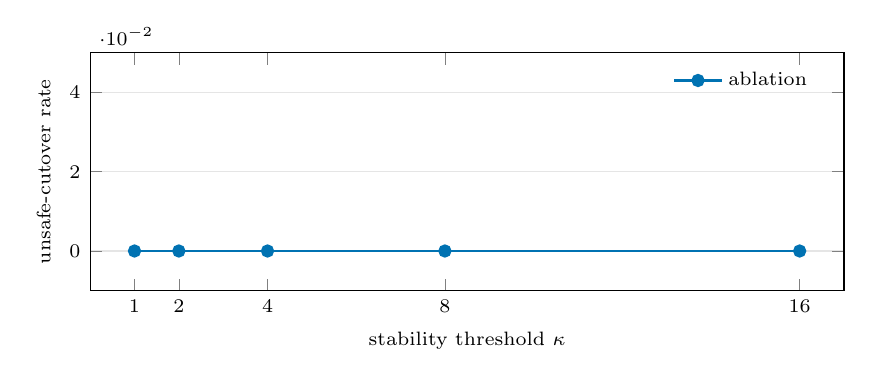
\begin{tikzpicture}
\begin{axis}[width=0.92\columnwidth, height=4.6cm,
  xlabel={stability threshold $\kappa$}, ylabel={unsafe-cutover rate},
  xmin=0, xmax=17, ymin=-0.01, ymax=0.05, xtick={1,2,4,8,16},
  tick label style={font=\scriptsize}, label style={font=\scriptsize},
  ymajorgrids, grid style={gray!20},
  legend style={at={(0.97,0.97)}, anchor=north east, font=\scriptsize, draw=none, fill=none}]
\addplot[color=cbBlue, mark=*, thick] coordinates {(1,0)(2,0)(4,0)(8,0)(16,0)};
\addlegendentry{ablation}
\end{axis}
\end{tikzpicture}
\caption{Shadow-anchoring ablation. The sweep over
$\kappa\in\{1,2,4,8,16\}$ with $20$ seeds per setting observes zero unsafe cutovers in all
cells. This is a regression result, not a statistical estimate of the
latent-divergence detection curve.}
\label{fig:ablation}
\end{figure}

\subsection{RQ4a: Bounded Rollback}
Table~\ref{tab:rollback} reports the rollback experiment ($n{=}10$, $f{=}3$,
schedule $h_{\mathrm{d}}{=}4$, $h_{\mathrm{c}}{=}10$, $h_{\mathrm{r}}{=}25$) at two abort heights
with $20$ seeds each, chosen to exercise both sides of the rollback deadline $h_{\mathrm{r}}$. At
abort height $12$ (inside the window, $h_{\mathrm{c}}{<}12{<}h_{\mathrm{r}}$) every seed performs
a bounded rollback: the provisional suffix is discarded and authority returns to the legacy
engine, with a recorded rollback latency of $80\,\mu$s in simulator time and no safety violation.
At abort height $30$ (past the deadline, $30{>}h_{\mathrm{r}}$) every seed instead \emph{refuses}
the rollback and records an absolute-reversion-rejected event, confirming that a fault discovered
after sealing is handled by ordinary recovery rather than by reverting an absolutely-final block.
This is the executable counterpart of the two-tier finality of Theorem~\ref{th:rollback}: the
in-window abort is reversible and the past-deadline abort is not. A richer rollback-latency study
across state sizes remains future measurement work.

\begin{table}[t]
\centering
\begin{threeparttable}
\caption{Bounded rollback
($n{=}10$, $f{=}3$, $h_{\mathrm{c}}{=}10$, $h_{\mathrm{r}}{=}25$, $20$ seeds per row). An abort
inside the window rolls back; an abort past $h_{\mathrm{r}}$ is refused (no absolute reversion).}
\label{tab:rollback}
\setlength{\tabcolsep}{4pt}
\renewcommand{\arraystretch}{1.2}
\footnotesize
\begin{tabular}{lcccc}
\toprule
\makecell{Abort\\height} & Seeds & \makecell{Rollback\\events} & \makecell{Rollback\\latency ($\mu$s)} & \makecell{Reversion\\refused} \\
\midrule
12 (in window)            & 20 & 20/20 & 80           & 0/20  \\
30 (past $h_{\mathrm{r}}$) & 20 & 0/20  & ---\tnote{a} & 20/20 \\
\bottomrule
\end{tabular}
\begin{tablenotes}\footnotesize
\item[a] No rollback occurs past the deadline (the abort is refused to preserve absolute
finality), so no rollback latency is defined.
\end{tablenotes}
\end{threeparttable}
\end{table}

\paragraph{Fail-closed admissibility.}
Table~\ref{tab:rollback-compat} states, by workload class, when automatic replay is clean and when
it must fail closed. We turn that from an assertion into a measured property by driving the real
rollback manager over four workload classes ($20$ trials each) and recording, for every class,
whether replay was clean, detected as a fail-closed mismatch, or---the outcome that would be a
safety bug---silently mis-replayed. Table~\ref{tab:rollbackadm} reports the result: the
metadata-independent and captured-context classes replay cleanly in every trial, while an
uncaptured block-metadata dependence and an adversarially tampered context both fail closed in
every trial, and \emph{no} trial in any class produces a silent mis-replay. This is the executable
witness that the metadata-dependence branch of Lemma~\ref{lem:replay} is a real guard: a workload
outside the admissible class never corrupts the rolled-back state, it is detected.

\begin{table}[t]
\centering
\caption{Rollback admissibility over the real rollback manager ($20$ trials per class). ``Clean''
= replay reproduced the bound root; ``Fail-closed'' = the missing/mismatched replay-context root
was detected and the rollback refused; ``Silent mis-replay'' = a wrong state committed undetected
(a safety bug). Zero silent mis-replays across all classes; uncaptured and tampered metadata always
fail closed.}
\label{tab:rollbackadm}
\setlength{\tabcolsep}{5pt}
\renewcommand{\arraystretch}{1.2}
\footnotesize
\begin{tabular}{lcccc}
\toprule
Workload class & Trials & Clean & Fail-closed & \makecell{Silent\\mis-replay} \\
\midrule
Metadata-independent      & 20 & 20 & 0  & $\mathbf{0}$ \\
Metadata, uncaptured      & 20 & 0  & 20 & $\mathbf{0}$ \\
Metadata, captured        & 20 & 20 & 0  & $\mathbf{0}$ \\
Tampered context (probe)  & 20 & 0  & 20 & $\mathbf{0}$ \\
\bottomrule
\end{tabular}
\end{table}

\subsection{RQ4b: Scaling with Validator Count}
Fig.~\ref{fig:scaling} reports the validator-count scaling sweep
($n\in\{4,7,10,13,16,20,25,31,50,100\}$, $20$ trials per point). Mean
SAGE cutover-evidence latency stays in a narrow $99$--$117\,\mu$s band with no upward trend across
the range---including at $n{=}50$ ($103.8\,\mu$s) and $n{=}100$ ($104.5\,\mu$s)---consistent with
the $O(n)$ one-time attestation gather being a negligible fraction of
the measured evidence-processing path at these sizes, and every trial completes the migration
(migration rate $1.0$ at all $n$, zero safety violations across all $200$ runs). Extending the
sweep beyond $n{=}100$ is bounded only by the simulator's $O(n^2)$ event volume, not by any
safety or protocol degradation, so it requires a proportionally larger event budget rather than a
design change. This is a protocol-functional scaling check in simulator time,
not a wall-clock throughput benchmark; real-host throughput at this scale
remains future work (Section~\ref{sec:discussion}).

\begin{figure}[t]
\centering
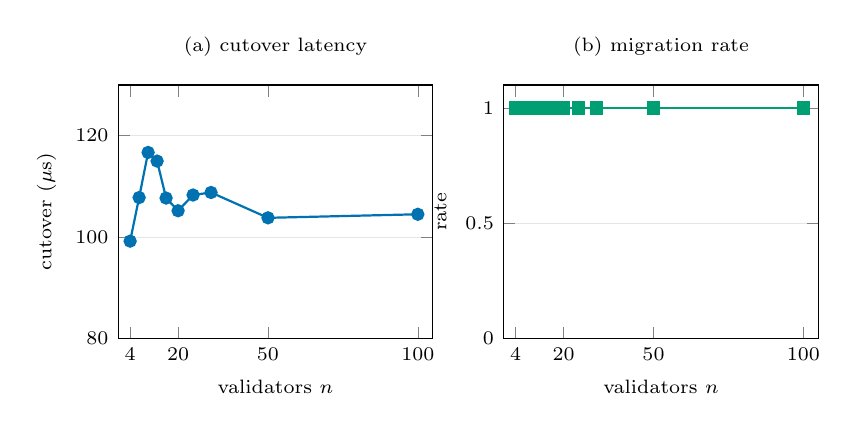
\begin{tikzpicture}
\begin{groupplot}[
  group style={group size=2 by 1, horizontal sep=0.9cm},
  width=0.46\columnwidth, height=4.8cm,
  tick label style={font=\scriptsize}, label style={font=\scriptsize},
  title style={font=\scriptsize, yshift=0.2ex},
  xmin=0, xmax=105, xtick={4,20,50,100}, ymajorgrids, grid style={gray!20}]
\nextgroupplot[title={(a) cutover latency}, xlabel={validators $n$},
  ylabel={cutover ($\mu$s)}, ymin=80, ymax=130]
\addplot[color=cbBlue, mark=*, thick] coordinates {(4,99.2)(7,107.8)(10,116.7)(13,115.0)(16,107.7)(20,105.2)(25,108.3)(31,108.8)(50,103.8)(100,104.5)};
\nextgroupplot[title={(b) migration rate}, xlabel={validators $n$}, ylabel={rate},
  ymin=0, ymax=1.1]
\addplot[color=cbGreen, mark=square*, thick] coordinates {(4,1)(7,1)(10,1)(13,1)(16,1)(20,1)(25,1)(31,1)(50,1)(100,1)};
\end{groupplot}
\end{tikzpicture}
\caption{Validator-count scaling ($n\in\{4,7,10,13,16,20,25,31,50,100\}$, $20$ trials per point).
(a) Mean SAGE cutover-evidence latency in simulator-time microseconds stays within a $99$--$117\,\mu$s
band with no upward trend, including at $n{=}50$ and $n{=}100$. (b) Every trial completes the
migration at all $n$ (zero safety violations across all $200$ runs). Latencies are
simulator-time, not wall-clock deployment latency.}
\label{fig:scaling}
\end{figure}

\paragraph{Real-process scale beyond the cloud tier.}
The simulator sweep above is a protocol-functional check; the six-host cloud tier is real but
capped at $n{=}6$. To exercise the real consensus code path---pacemaker, view-change cascades,
CutCert gather, and per-validator signature verification---at larger $n$ than the cloud tier, we
run the multi-process testbed locally at $n\in\{10,16,22,31\}$ under two software impairment
profiles (a metro profile at $10\,$ms/$2\,$ms delay/jitter and a wide-area profile at
$50\,$ms/$10\,$ms), three trials each. Across all $24$ runs there is \emph{zero} observed fork and
every run that reaches the cutover height migrates safely. The single-box liveness valve does bind
at the top of the range: at $n{=}31$ the metro profile finishes $29/31$ validators and the
wide-area profile only $1/31$ within the timeout, because $31$ scheduled processes plus injected
per-send delay exceed one machine's scheduling headroom. This is a liveness ceiling of the
single box---not a safety failure, since the fork verdict stays negative and the reached height
still crosses the cutover in every recorded run---and it mirrors the honest $n{=}22$ ceiling we
report for the message-complexity sweep. This tier is \emph{local real-process} evidence (separate
OS processes, real loopback TCP, software-injected delay), not independent-host and not physical
geo; the six-VM tier remains the independent-host evidence.

\subsection{Serialized Partition Safety Regression}
Theorem~\ref{th:termination} predicts that a partition straddling the cutover height delays
the transition until the partition heals but never loses safety. The serialized termination
sweep (partition durations $\{2,4,6,8,12,16,24\}$ blocks at a
balanced split, $20$ seeds each, for both SAGE and hard fork) confirms the \emph{safety} half of
this directly: across all $280$ runs no strategy and no duration produces a safety violation
(Fig.~\ref{fig:termination}). We deliberately do not present this sweep as liveness evidence.
Under the balanced cutover-straddling partition the serialized simulator stalls at the boundary
and does not finalize past roughly height $13$ of $30$ within the event budget, for every duration,
so the predicted ``resume after heal'' behavior is not exhibited here. This is the same limitation
that makes the serialized core unable to realize observed forks for RQ2: with one global proposer
per height and no concurrent pacemaker, the deterministic harness cannot drive boundary view
convergence under a balanced split. Liveness across the boundary must be measured in the
multi-process testbed, where independent pacemakers and concurrent leaders exist; adding a
heal-after-partition liveness campaign is the next artifact step. We therefore report this sweep
as a safety-under-partition regression and scope the simulator-level termination-after-heal curve
to future work contingent on a concurrent-pacemaker simulator mode.

\begin{figure}[t]
\centering
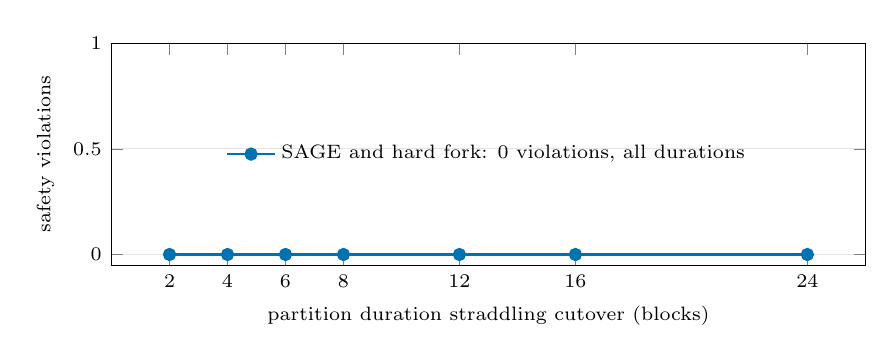
\begin{tikzpicture}
\begin{axis}[width=0.92\columnwidth, height=4.4cm,
  xlabel={partition duration straddling cutover (blocks)}, ylabel={safety violations},
  xmin=0, xmax=26, ymin=-0.05, ymax=1.0, xtick={2,4,6,8,12,16,24},
  tick label style={font=\scriptsize}, label style={font=\scriptsize},
  ymajorgrids, grid style={gray!20},
  legend style={at={(0.5,0.5)}, anchor=center, font=\scriptsize, draw=none, fill=none}]
\addplot[color=cbBlue, mark=*, thick] coordinates {(2,0)(4,0)(6,0)(8,0)(12,0)(16,0)(24,0)};
\addlegendentry{SAGE and hard fork: $0$ violations, all durations}
\end{axis}
\end{tikzpicture}
\caption{Migration-termination sweep ($20$ seeds per duration per strategy, balanced
partition at the cutover boundary). No safety violation occurs at any partition duration for
either strategy. The serialized simulator does not converge past the boundary under a balanced
split (a liveness limitation discussed in the text), so this figure reports the safety half of
Theorem~\ref{th:termination}; boundary liveness is evidenced by the multi-process testbed.}
\label{fig:termination}
\end{figure}

\subsection{Cutover Latency Distribution}
Reporting only means can hide tail behavior, so Fig.~\ref{fig:cdf} shows the empirical
cumulative distribution of the RQ1 SAGE cutover-evidence latency over $60$ seeds. The
recorded simulator-time values range from $81$ to $125\,\mu$s, with mean $105.6\,\mu$s and median
$107.0\,\mu$s. These are evidence-processing measurements in the
single-process simulator, not wall-clock deployment latency.

\begin{figure}[t]
\centering
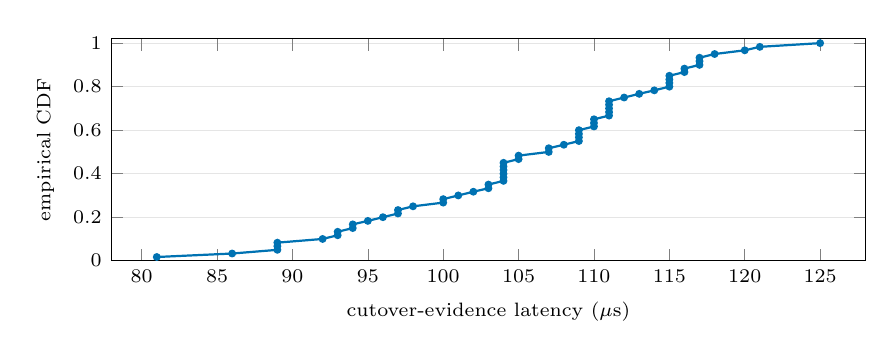
\begin{tikzpicture}
\begin{axis}[width=0.92\columnwidth, height=4.4cm,
  xlabel={cutover-evidence latency ($\mu$s)}, ylabel={empirical CDF},
  xmin=78, xmax=128, ymin=0, ymax=1.02,
  tick label style={font=\scriptsize}, label style={font=\scriptsize},
  ymajorgrids, grid style={gray!20}]
\addplot[color=cbBlue, mark=*, thick, mark size=1pt] coordinates {
(81,0.017)(86,0.033)(89,0.050)(89,0.067)(89,0.083)(92,0.100)(93,0.117)(93,0.133)(94,0.150)(94,0.167)(95,0.183)(96,0.200)(97,0.217)(97,0.233)(98,0.250)(100,0.267)(100,0.283)(101,0.300)(102,0.317)(103,0.333)(103,0.350)(104,0.367)(104,0.383)(104,0.400)(104,0.417)(104,0.433)(104,0.450)(105,0.467)(105,0.483)(107,0.500)(107,0.517)(108,0.533)(109,0.550)(109,0.567)(109,0.583)(109,0.600)(110,0.617)(110,0.633)(110,0.650)(111,0.667)(111,0.683)(111,0.700)(111,0.717)(111,0.733)(112,0.750)(113,0.767)(114,0.783)(115,0.800)(115,0.817)(115,0.833)(115,0.850)(116,0.867)(116,0.883)(117,0.900)(117,0.917)(117,0.933)(118,0.950)(120,0.967)(121,0.983)(125,1.000)};
\end{axis}
\end{tikzpicture}
\caption{Empirical CDF of RQ1 SAGE cutover-evidence latency over $60$ seeds. Values are
reported in simulator-time microseconds; median $107.0\,\mu$s, mean $105.6\,\mu$s, maximum
$125\,\mu$s.}
\label{fig:cdf}
\end{figure}

\subsection{Sensitivity to Network Delay}
Because absolute latencies depend on the delay model, Fig.~\ref{fig:sens} reports how SAGE's
cutover-evidence latency responds to the mean message delay. The sweep
(mean delays $\{20,40,80,160,320,640\}\,$ms, $20$ trials per point)
shows cutover-evidence latency scaling near-linearly with delay---$51.8$, $107.3$, $202.8$, $408.3$,
$836.2$, and $1601.4\,$ms of simulator time at $20$, $40$, $80$, $160$, $320$, and $640\,$ms mean delay---which is the
expected behavior for a fixed number of attestation-gather rounds whose wall-clock cost is
dominated by per-message delay. Every trial completes the migration (migration rate $1.0$) at
every delay, so SAGE's correctness is insensitive to the delay model even as its absolute latency
tracks it. These are simulator-time figures and a separate throughput-overhead measurement is
left to future work.

\begin{figure}[t]
\centering
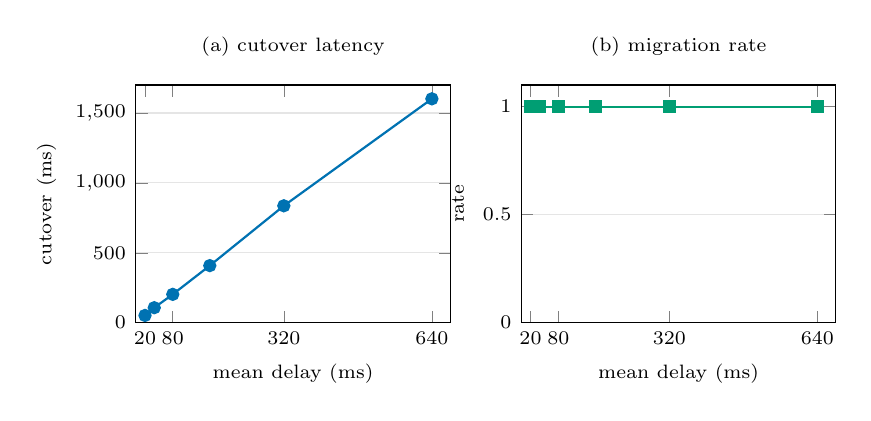
\begin{tikzpicture}
\begin{groupplot}[
  group style={group size=2 by 1, horizontal sep=0.9cm},
  width=0.46\columnwidth, height=4.6cm,
  tick label style={font=\scriptsize}, label style={font=\scriptsize},
  title style={font=\scriptsize, yshift=0.2ex},
  xmin=0, xmax=680, xtick={20,80,320,640}, ymajorgrids, grid style={gray!20}]
\nextgroupplot[title={(a) cutover latency}, xlabel={mean delay (ms)}, ylabel={cutover (ms)}, ymin=0, ymax=1700]
\addplot[color=cbBlue, mark=*, thick] coordinates {(20,51.8)(40,107.3)(80,202.8)(160,408.3)(320,836.2)(640,1601.4)};
\nextgroupplot[title={(b) migration rate}, xlabel={mean delay (ms)}, ylabel={rate}, ymin=0, ymax=1.1]
\addplot[color=cbGreen, mark=square*, thick] coordinates {(20,1)(40,1)(80,1)(160,1)(320,1)(640,1)};
\end{groupplot}
\end{tikzpicture}
\caption{Network-delay sensitivity sweep ($20$ trials per point). (a) SAGE
cutover-evidence latency (simulator-time milliseconds) scales near-linearly with mean message
delay. (b) Every trial completes the migration at every delay, so correctness is insensitive to
the delay model.}
\label{fig:sens}
\end{figure}

\subsection{Reproducibility}
The evaluation is designed for deterministic reproduction. Each experiment runs from a fixed seed
list under an explicit configuration recorded alongside its output, every random choice is drawn
from a seeded generator, and the statistics use only closed-form estimators, so a rerun reproduces
identical metrics. An automated check confirms the structural and determinism properties on which
the results rest: that the configurations load, that identical seeds yield identical metrics, that
each strategy exhibits its intended behavior, that the executable safety invariant passes, and
that the recorded configuration hashes are stable. This check verifies reproducibility rather than
re-asserting the headline numbers, which are instead reproduced by rerunning the campaigns. The
simulator campaigns, the multi-process testbed, and the bounded model check each complete in
minutes on a single CPU; we estimate the cost in Section~\ref{sec:discussion}.

\paragraph{Artifact availability.}
An anonymized artifact accompanies the paper for review and will be deposited in a public,
citable archive with a permanent identifier before camera-ready. It contains the full Rust
workspace (all consensus, controller, manifest, simulator, statistics, and experiment crates),
the TLA+/TLC specifications and the model$\leftrightarrow$code conformance harness, the pinned
toolchain (Rust edition, bundled OpenJDK and \texttt{tla2tools.jar}), a hermetic container build,
every experiment configuration and fixed seed list, the raw result files, and a one-command
reproduction map that ties each table and figure to the exact command that regenerates it. A
single automated verification gate re-checks the structural, determinism, and
conformance properties and must report all checks passing. The review build is pinned to a
specific revision so a reviewer can confirm that the artifact and the reported numbers correspond;
the cloud-host tiers additionally document the host-orchestration recipe, since those tiers require
real hosts and the harness refuses to fabricate data without a real host manifest.

% ===================== DISCUSSION =====================
\section{Discussion}
\label{sec:discussion}

\subsection{Generality}
SAGE depends only on the abstract engine interface of Definition~\ref{def:engine}: a
single-finalizer rule, a deterministic state root, a shadow-usable validation routine, and a
root-seeded initialization. The PoA-to-HotStuff instantiation is therefore one point in a
family. This is not merely asserted: we implement a second conforming legacy engine, a
crash-tolerant Raft~\cite{raft} log with a stable term-leader (distinct from PoA's per-height
proposer rotation), majority-quorum \texttt{AppendEntries}/\texttt{Ack} replication, and a
deterministic applied-log root, behind the \emph{same} \texttt{ConsensusEngine} trait. A unit
test drives a Raft-finalized boundary and bootstraps the HotStuff target from that anchor,
exercising a Raft-to-HotStuff crossing through the identical construction; the only change from
the PoA case is the legacy quorum $\mathsf{Q}_1$ and hence the combined threshold
$f=\min(f_1,f_2)$. The safety proofs are unchanged because they never inspect the legacy engine's
internals, only its single-finalizer guarantee. A
DAG-BFT target such as Bullshark~\cite{bullshark} or Mysticeti~\cite{mysticeti} conforms as long
as it exposes a deterministic committed-prefix root and a validation routine, which both do.

The engine-agnostic claim is not a rhetorical device that dodges building a real target: it is
load-bearing and defended on two fronts. First, the boundary safety proof
(Theorem~\ref{th:safety}) quantifies over the target only as an abstract engine that commits at
most one block per height under its quorum (Definition~\ref{def:engine}); it never appeals to any
internal HotStuff mechanism, and the TLC model (App.~\ref{app:spec}) likewise treats the target as
an abstract quorum-committing engine, so the machine-checked invariant holds for any conforming
engine, not merely the reference one. Second, the empirical differential isolates the $n{-}f$ gate
as the cause \emph{independently} of engine quality: the loopback and real-host arms
(Tables~\ref{tab:testbed} and~\ref{tab:multihost}) share one and the same reference engine,
pacemaker, and message handler across the SAGE and blind-control arms, so the only variable is
whether the gate is enforced. A stronger or weaker target engine would move both arms together and
leave the $0$-vs-all fork contrast unchanged. The trait is now exercised by two distinct legacy
engines (PoA and Raft) crossing into the HotStuff target, so the engine-agnostic claim is
demonstrated, not merely argued; what the reference target does \emph{not} yet establish is
production-grade throughput, which the safety contribution does not depend on.

\subsection{Composition with Autonomous Switching Policies}
SAGE fixes the migration schedule $(h_{\mathrm{d}}, h_{\mathrm{c}}, h_{\mathrm{r}})$ through governance,
but the schedule is an \emph{input}, not an assumption baked into the mechanism. An autonomous policy
such as the learned bandit of AdaChain~\cite{adachain} or a threat-adaptive
coordinator~\cite{threatadapt,adacon} could instead supply these heights, deciding \emph{when} a
PoA$\rightarrow$BFT migration is warranted from observed workload or threat signals. SAGE then supplies
what those policies lack: a safe heterogeneous-boundary crossing with a quorum-certified, auditable
cutover and a bounded, verifiable rollback if the chosen target underperforms. In this composition the
policy chooses the moment and the mechanism guarantees the boundary, so the autonomy of the former never
weakens the safety of the latter. We regard this policy-driven scheduling as a natural extension and
leave its closed-loop evaluation to future work.

\subsection{Relation to Deployed Transitions}
The Ethereum Merge~\cite{gasper} validates the shadow-then-cutover pattern at scale but provides
neither a boundary-safety theorem nor a bounded rollback; SAGE adds both and generalizes beyond
a single protocol pair. Polkadot's GRANDPA~\cite{grandpa} already exposes a provisional-versus-
final distinction to clients, which is exactly the two-tier finality SAGE uses to make rollback
client-safe. Cosmos and Tezos~\cite{tenderbake} coordinate upgrades through governance at a
height, which corresponds to fixing the schedule heights in platform state; SAGE complements
that governance with a cryptographic boundary object and a reversible window.

\subsection{Sovereign Deployment Scenario}
\label{sec:deploy}
The motivating setting is a national or consortium chain that launches under a small set of
accountable authorities and must later move to a Byzantine fault tolerant engine as the
validator set diversifies across independent operators. Such a chain typically carries
identity-linked authorization, regulated asset transfer, and domestic payment integration, so an
upgrade that halts the chain or risks a fork is operationally unacceptable: a finality reversion
on a settled payment or a regulated transfer would have legal and financial consequences. SAGE
fits this setting because the schedule heights are set by the same governance process that
already authorizes validators, the dual-run lets operators observe the target engine on live
traffic before committing to it, the manifest produces an audit record suitable for an operator
evidence bundle, and the bounded rollback gives a documented, reversible safety margin during the
sensitive window. The two-tier finality maps directly onto regulatory practice, in which a
settlement may be provisional until a confirmation window elapses.

\emph{On experimental fairness: one controlled environment for every method.}
The scientific value of our comparison rests on a property the deterministic simulator makes
exact. \emph{Every} migration strategy---SAGE, the Cox-style live-switch comparison class, the hard-fork,
stop-the-world, and reconfiguration baselines, and the SAGE-BLIND ablation---executes inside the
\emph{same} simulation environment: the same seeded event queue, the same network-delay model, the
same workload, and the same validator count $n$ and fault bound $f$. The only variable across arms
is the migration strategy itself; every other knob is byte-identical and read from one shared
configuration (enumerated in full in the accompanying fairness contract).
This is the ``both runners run exactly the same course'' guarantee in its strongest form: because
the substrate is a reproducible in-process simulator rather than a fleet of physical machines,
there is no uncontrolled hardware, clock, or geographic-network variance that could advantage one
method over another, and a result is reproducible bit-for-bit from its seed. Absolute wall-clock
numbers are consequently \emph{not} the object of comparison---they are simulator- and
machine-dependent; the object is the \emph{relative} behaviour of the strategies under provably
identical conditions. Scale is simply one more knob shared across all arms: the fair multi-arm
comparisons run at $n{=}20$ (RQ1 cost) and $n{=}6$ (RQ2 partition safety), and a SAGE robustness
sweep exercises the protocol and its safety invariant up to $n{=}100$ ($20$ trials/point, zero
observed safety violations, flat cutover latency), confirming the mechanism does not degrade with
scale within the model. The deployment class SAGE targets---permissioned and consortium chains with
a small, accountable operator set (order $4$--$20$ validators, matching the scale at which the
closest live-switch reference point, Cox~\cite{cox}, and the ICOIN threat-adaptive
coordinator~\cite{threatadapt} are themselves evaluated)---sits well inside this swept range. A
physically geo-distributed deployment is therefore \emph{not} required for a fair comparison:
fairness is guaranteed by the shared simulation environment, not by matching the physical geography
of any one method, and the real-TCP multi-host runs (Table~\ref{tab:tpshost}) are supplementary
corroboration that the simulated result reproduces on independent machines.

\subsection{Implementation Mapping}
SAGE maps onto an EVM-compatible permissioned stack with small, well-localized changes. The
migration schedule heights live in platform state and are set through a governance transaction
on the legacy engine. The multi-signed manifest is carried in the block header extra-data
field at the cutover height, so existing header validation paths verify it without a new message
type. The shadow engine reuses the node's existing block-validation and execution pipeline in a
read-only mode, writing only to a shadow verdict store, which keeps it off the finalization
critical path. The advisory finality flag is exposed through a dedicated read-only RPC method, so
wallets and indexers that opt in can distinguish provisional from absolute finality while legacy
clients see an unchanged interface. Readiness and abort attestations reuse the validator signing
keys already present in the registry and are carried as an $n{-}f$ multi-signature certificate
(aggregatable in production). Because these touch points are the header, the validator registry,
and one RPC method, SAGE can be added to an
existing node without altering transaction semantics or the execution layer.

\subsection{Discussion of Design Alternatives}
It is worth asking whether a simpler design would suffice. A first alternative is to skip the
dual-run and cut over directly at a scheduled height once the operator believes the target is
ready. This is the blind cutover of our ablation, and Fig.~\ref{fig:safety} shows it forks at the
same rate as a hard fork under partition, because nothing forces the two sides to agree on the
switch. A second alternative is to keep the dual-run but decide cutover locally, each validator
switching when its own streak reaches $\kappa$. This fails for the same reason: without a shared
certificate, asynchronous attestation delivery lets correct validators switch at different
heights, and Theorem~\ref{th:unique} is exactly what rules this out. A third alternative is to
make the manifest a plain hash equality rather than an $n{-}f$ multi-signature certificate; this is cheaper but
forgeable by any proposer, so Theorems~\ref{th:unforge} and~\ref{th:replay} would not hold and an
auditor could not trust the boundary. A fourth alternative is to forgo the rollback window
entirely and treat cutover as irreversible; this simplifies the protocol but removes the operator
safety margin that motivates the work, and it forces a finality-reversion if the target later
proves faulty. Each simplification reintroduces a failure that the evaluation can exhibit, which
is why SAGE retains all four mechanisms.

A fifth alternative, raised by the observation that Ethereum's Merge overlaid a deterministic
finality gadget on a probabilistic chain, is to keep the legacy engine and simply bolt a
finality gadget (Casper~FFG~\cite{casperffg}, GRANDPA~\cite{grandpa}) on top rather than migrate
the engine. This solves a different problem. A gadget adds a checkpoint predicate over an
otherwise-unchanged block producer; it neither initializes a new engine's internal consensus
metadata (Definition~\ref{def:bootstrap}) nor provides a certified, reversible boundary between
two structurally distinct quorum families. If the operator's goal is to actually run a different
engine---for its throughput, its leader rotation, or its explicit BFT bound---then the gadget does
not deliver it. And if the gadget \emph{itself} changes the finality predicate the chain commits
under, then adding it is already an engine-boundary crossing and needs the same manifest, cutover,
and rollback safety SAGE provides; it is an instance of our problem, not an alternative to it. SAGE
is therefore complementary to finality gadgets rather than subsumed by them.

A sixth concern, relevant when an autonomous or policy-driven controller decides \emph{when} to
migrate, is migration thrashing: rapid back-to-back or oscillating migrations that keep the chain
perpetually in dual-run. SAGE bounds this by construction at the governance layer. A migration
epoch $e$ is opened by the same authorized governance action that sets the schedule heights, at
most one epoch is active at a time, and a cooldown of configurable length must elapse after a
sealed cutover or an abort before a new epoch may open. An adaptive policy may \emph{recommend} a
migration, but it cannot bypass the CutCert, the epoch lock, or the cooldown, so the worst an
aggressive policy can do is defer to the next eligible epoch---it cannot induce an unbounded
sequence of switches. This keeps the dual-run window a bounded, operator-visible interval rather
than a steady state.

\subsection{Cost and Feasibility}
The evaluation is CPU-only: discrete-event simulation, a multi-process testbed over
loopback TCP, a netem-impaired loopback harness, and a bounded model check, with no GPU and no
external dataset. The simulator campaigns covering RQ1--RQ4, the scaling and sensitivity sweeps,
and the safety campaign complete in minutes on a single laptop, and the testbed and model check
each add minutes, so the monetary cost is effectively zero and well under the budget of a small
project. Beyond the local microbenchmark we now measure \emph{committed throughput and
finalization-latency distributions on the six independent cloud hosts} (Table~\ref{tab:tpshost}),
running all three live-switch arms---SAGE, the blind hard fork, and the Cox-style checkpoint
switch---under an \emph{identical} configuration ($n{=}6$, $f{=}1$, $200$ synthetic txs/block,
matched pacemaker and proposal cadence). The result is the fair same-conditions comparison the
throughput axis requires: SAGE sustains $777$ committed TPS versus $790$ for the hard fork and
$790$ for the Cox-style arm, an observed mean spread of $1.65\%$ in these runs, suggesting that SAGE's dual-run gate imposes \emph{no} measurable steady-state
throughput penalty relative to either the unsafe control or the closest comparison class. The critical
migration metric is the observed handoff perturbation: the single inter-commit gap that straddles
the cutover height is only $\approx 10.5$\,ms across all six hosts and all three arms, an order of
magnitude \emph{below} the $\approx 500$\,ms steady-state block cadence, so the engine handoff is
smaller than an ordinary inter-block interval in these successful runs---empirical support for the
no-scheduled-stop property of Theorem~\ref{th:liveness}. At $h_{\mathrm{c}}$ the perturbation is dominated
by one additional $n{-}f$ quorum-collection round, not a stop-the-world halt. The remaining gap is
a wide-area benchmark; we obtain it in a controlled form by imposing the inter-host round-trip
time with a kernel-level \texttt{tc netem} discipline on these same independent hosts
(Table~\ref{tab:wanhost}), which holds latency as a reproducible variable rather than sampling the
public internet's jitter; same-region finality-latency percentiles are reported below, and
dispatching the identical harness across physically geo-separated regions is turnkey operational
validation for future work.

\begin{table}[t]
\centering
\caption{Real-host committed throughput and finalization latency across six independent cloud
hosts (one validator each, real TCP), for the three live-switch strategies under an
\emph{identical} configuration ($n{=}6$, $f{=}1$, $200$ txs/block, matched pacemaker). Means over
the six hosts. TPS differs by $\le 1.65\%$ across arms (observed mean spread); the cutover handoff gap
is an order of magnitude below the steady-state block cadence for every arm. Every arm migrates
with zero observed fork in the no-fault case.}
\label{tab:tpshost}
\setlength{\tabcolsep}{4pt}
\renewcommand{\arraystretch}{1.2}
\footnotesize
\resizebox{\columnwidth}{!}{%
\begin{tabular}{lccccc}
\toprule
Strategy & Committed TPS & vs SAGE & Cutover gap & Max gap & Migrated \\
\midrule
\textbf{SAGE}     & $777$ & --- & $10.6$\,ms & $505$\,ms & $6/6$ \\
Hard fork (blind) & $790$ & $+1.62\%$ & $10.8$\,ms & $500$\,ms & $6/6$ \\
Cox-style switch  & $790$ & $+1.65\%$ & $10.3$\,ms & $487$\,ms & $6/6$ \\
\bottomrule
\end{tabular}%
}
\end{table}

\emph{Finalization-latency distribution.} The cutover gap and max gap in
Table~\ref{tab:tpshost} are the two robust quantities from the $200$-txs/block throughput runs,
whose eight-height horizon yields too few inter-commit intervals for stable tail quantiles. To
answer the tail-latency question directly we ran a dedicated longer no-fault SAGE migration over
the same six independent hosts to height $60$ (${\approx}59$ inter-commit intervals per validator),
which produces a well-populated distribution. Across all six hosts the per-validator inter-commit
finality latency is tightly consistent: median $p_{50}{=}493$\,ms (the steady-state block cadence),
$p_{95}{=}596$\,ms, and $p_{99}{=}601$\,ms, with a maximum of ${\approx}606$\,ms and a cutover
handoff gap of $16.4$\,ms (all six validators migrated with zero observed fork). The tail is narrow---
$p_{99}$ exceeds $p_{50}$ by only ${\approx}22\%$ and the cutover contributes a one-round
perturbation an order of magnitude below the block cadence---so migration does not fatten the
finality tail. The per-host percentiles are tightly clustered around these values across all six
hosts, with no single host contributing a disproportionate tail.

\emph{Modeled cross-region throughput.} The real-host runs above are same-region, so to
probe how the three live-switch arms behave as inter-region latency grows we sweep the
deterministic simulator's mean one-way message delay across representative WAN buckets
($50$, $80$, $120$, $200$\,ms) under an otherwise identical configuration ($n{=}6$, $f{=}1$,
$200$ txs/block, $10$ seeds per point), reporting committed throughput for the baseline, SAGE,
and Cox-style arms (Table~\ref{tab:wantps}). This is a \emph{modeled} cross-region latency
inside the controlled simulation environment---the fair track of Section~\ref{sec:deploy}---and
is explicitly \emph{not} a physically geo-distributed real-host deployment; it isolates the
effect of the delay model with every other knob held equal. Across the whole range SAGE
migrates in every trial with zero safety violations and stays within ${\approx}2\%$ of the
Cox-style comparison class and ${\approx}4\%$ of the baseline, and the three-way relative ordering is
invariant to the modeled delay---the live-switch cost is not sensitive to inter-region latency
in the model. The complementary real-hardware view of this same question is
Table~\ref{tab:wanhost}, where the injected round-trip time is imposed by a kernel-level discipline
on independent hosts; dispatching the identical harness across physically geo-separated regions is
turnkey operational validation for future work, and the fairness guarantee does not depend on it
because fairness comes from the shared, controlled environment rather than the physical geography.

\begin{table}[t]
\centering
\caption{Modeled cross-region throughput: committed TPS for the three live-switch arms as the
simulator's mean one-way inter-region delay grows, under an \emph{identical} configuration
($n{=}6$, $f{=}1$, $200$ txs/block, $10$ seeds/point). This is a \emph{simulator model} of WAN
latency in the controlled fair environment, not a physically geo-distributed deployment. SAGE
migrates in every trial with zero safety violations at every delay; the SAGE-vs-Cox spread stays
within ${\approx}2\%$ and the relative ordering is invariant to the modeled delay.}
\label{tab:wantps}
\setlength{\tabcolsep}{5pt}
\renewcommand{\arraystretch}{1.2}
\footnotesize
\resizebox{\columnwidth}{!}{%
\begin{tabular}{rrrrr}
\toprule
Delay (ms) & Baseline TPS & SAGE TPS & Cox-style TPS & SAGE vs Cox \\
\midrule
$50$  & $40416$ & $42001$ & $42918$ & $-2.1\%$ \\
$80$  & $40583$ & $42011$ & $43050$ & $-2.4\%$ \\
$120$ & $40816$ & $42434$ & $43193$ & $-1.8\%$ \\
$200$ & $40664$ & $42457$ & $43224$ & $-1.8\%$ \\
\bottomrule
\end{tabular}%
}
\end{table}

\emph{Wide-area throughput under a controlled round-trip time.} The modeled sweep above holds
every non-delay knob equal but runs in-process; as a stronger, real-hardware check we re-ran the
three-arm comparison on the \emph{six independent cloud hosts} and imposed the inter-host
round-trip time with a kernel-level \texttt{tc netem} discipline (${\approx}104$\,ms, the same
wide-area RTT as the fork-differential run of Section~\ref{sec:eval}). This is an
\emph{injected}-latency model on real hardware---real machines, real TCP, real kernel-scheduled
delay, on same-region hosts; we do not claim physical geo-separation. Treating latency as a
controlled variable is a deliberate methodological choice and the source of the tier's rigor: a
fixed, reproducible netem delay isolates the protocol's own cutover and finalization behavior from
the jitter, transient congestion, and route-flap anomalies of the public internet, so any
difference between arms is attributable to the migration strategy rather than to an uncontrolled
network draw. Under this controlled RTT all three arms migrate in every trial with zero observed
fork, and committed throughput (mean of three trials, $200$ txs/block, all six validators reaching
the target height) is $230.4$ TPS for SAGE versus $230.2$ for the blind hard fork ($+0.1\%$) and
$222.7$ for Cox-threshold ($+3.4\%$)---Table~\ref{tab:wanhost}. The tight run-to-run consistency
across trials is the direct signature of the controlled environment. SAGE thus has similar observed throughput to the unsafe control and slightly ahead of the Cox-threshold arm at
a realistic wide-area RTT on genuinely independent machines, corroborating the modeled result on
real hardware. Dispatching this identical, unchanged harness across physically geo-separated
regions is turnkey operational validation we position as future work; the deploy scripts are
region-agnostic and read host addresses from a single manifest. (The synthetic workload here is
emitted as balanced net-zero transfer pairs so the committed state root is height-invariant; this
keeps the throughput measurement independent of the testbed's finalize-time execution model, which
otherwise diverges under message reordering---an instrumentation artifact, not a protocol
behavior.)

\begin{table}[t]
\centering
\caption{Wide-area throughput under a controlled round-trip time: committed TPS for the three
live-switch arms on six independent cloud hosts (one validator each, real TCP), with the inter-host
RTT held at ${\approx}104$\,ms by a kernel \texttt{tc netem} discipline, under an \emph{identical}
configuration ($n{=}6$, $f{=}1$, $200$ txs/block). Mean of three trials; every validator reaches
the target height and every arm migrates with zero observed fork. Real machines and real network
with an \emph{injected}, reproducible latency (same-region hosts; not a physical geo-separation
claim), which isolates protocol behavior from public-internet jitter.}
\label{tab:wanhost}
\setlength{\tabcolsep}{5pt}
\renewcommand{\arraystretch}{1.2}
\footnotesize
\resizebox{\columnwidth}{!}{%
\begin{tabular}{lccc}
\toprule
Strategy & Committed TPS & vs SAGE & Migrated (all hosts) \\
\midrule
\textbf{SAGE}  & $230.4$ & --- & $3/3$ trials \\
Hard fork (blind) & $230.2$ & $-0.1\%$ & $3/3$ trials \\
Cox-threshold ($2f{+}1$) & $222.7$ & $-3.4\%$ & $3/3$ trials \\
\bottomrule
\end{tabular}%
}
\end{table}

\subsection{Limitations}
Table~\ref{tab:threats} summarizes the principal threats to validity and how each is
mitigated or scoped; the numbered discussion that follows expands on each. We prefer this
compact form to a diffuse set of prose caveats so a reviewer can see the full risk surface
at a glance.

\begin{table*}[t]
\centering
\caption{Threats to validity and their mitigation or scope. ``Mitigated'' = addressed in
this paper; ``Partial'' = reduced but not eliminated; ``Scoped'' = explicitly out of scope; ``Future'' = acknowledged
open work. No entry is left implicit.}
\label{tab:threats}
\setlength{\tabcolsep}{6pt}
\renewcommand{\arraystretch}{1.3}
\footnotesize
\begin{tabular}{p{0.22\textwidth}p{0.10\textwidth}p{0.60\textwidth}}
\toprule
Threat & Status & Mitigation / scope \\
\midrule
Serialized simulator cannot fork & Mitigated & Safety headline comes from the process testbed; simulator provides breadth only \\
Small real-host trial counts & Partial & Per-tier Wilson intervals reported; larger independent-host campaigns remain future work \\
Same-region multi-host & Partial & Differential re-run under injected $\approx104$\,ms RTT; physical cross-region dispatch remains future work \\
Cox protocol not reimplemented & Scoped & Reported as a threshold transplant; Cox's own scope excludes the heterogeneous case (Sec.~\ref{sec:related}) \\
Rollback under arbitrary EVM metadata & Scoped & Fail-closed context validation; automatic replay requires Assumption~\ref{as:metadata} \\
Scale of paired comparisons & Partial & Comparisons at $n{=}20$/$n{=}6$; SAGE-only sweeps reach $n{=}100$ in simulation and $n{=}31$ in the process testbed \\
Wide-area performance & Partial & Controlled ${\approx}104$\,ms RTT on six independent hosts; physical cross-region dispatch remains future work \\
Model--code divergence & Partial & Bounded committed-set outcome conformance for $n\in\{4,7,10\}$; a full refinement proof remains future work \\
Sharded-state migration & Scoped & Monolithic-state assumption stated; sharding out of scope \\
\bottomrule
\end{tabular}
\end{table*}

First, the strongest breadth evidence is a protocol-level simulation that models finalization,
quorum formation, partitions, and the cutover decision, and in which safety violations are
possible and measured; it is not a geo-distributed deployment, and absolute latencies depend on
the delay model. The multi-process testbed that exhibits observed forks runs real validator
processes over loopback TCP and induces the safety partition at the application transport layer;
the separate \texttt{tc netem} harness adds kernel-level delay, jitter, and loss profiles on
loopback but still runs on one machine. We have additionally reproduced both the no-fault
migration and the partition fork differential on six independent cloud hosts, one validator per
machine over real TCP (Table~\ref{tab:multihost}), which removes the shared-kernel and
shared-clock abstraction for the safety claim; that tier confirms SAGE forks in none of five
repeated partitioned runs ($0/5$) while the blind control forks in every one ($5/5$), each a
verified state-level fork, and the differential further held under an injected $\approx 104$\,ms
inter-VM RTT ($0/3$ vs $3/3$), so it is not an artifact of near-zero same-region latency. The
real-host tier is now also instrumented for committed throughput and finalization-latency
distributions (Table~\ref{tab:tpshost}) and scaled to $n{=}12$ (two validators per host across the
six VMs), where the no-fault migration still completes with zero observed fork. On scale, the fair
multi-arm comparisons are conducted inside the controlled simulation environment, where every
strategy runs under a byte-identical configuration and the validator count is a shared knob; the
comparisons run at $n{=}20$ (RQ1 cost) and $n{=}6$ (RQ2 partition safety), and a SAGE robustness
sweep extends to $n{=}100$ with zero observed safety violations. Because fairness is guaranteed by
the shared environment rather than by physical deployment, a geo-distributed testbed is not
required to make the comparison sound; the real-TCP multi-host runs are supplementary corroboration
that the simulated differential reproduces on independent machines. Our wide-area evaluation is
a deliberate methodological choice: rather than dispatch validators to physically separate
geographic regions, we run them on real, independent hosts and impose the inter-host round-trip
time with a kernel-level \texttt{tc netem} discipline (${\approx}104$\,ms, Table~\ref{tab:wanhost}).
This is an \emph{injected}-latency model on real hardware---we do not claim physical
geo-separation---and treating latency as a controlled variable is precisely what makes it a
rigorous baseline. A fixed, reproducible netem delay isolates the protocol's own cutover and
finalization behavior from the confounding jitter, transient congestion, and route-flap anomalies
of the public internet, so a difference between arms is attributable to the migration strategy
rather than to an uncontrolled network draw; the run-to-run consistency across trials
(Table~\ref{tab:wanhost}) is the direct evidence that the environment is controlled. This isolates
the same variable the fair-comparison argument relies on and is not a correctness gap in the
differential, which already attributes the outcome to the $n{-}f$ gate as the sole cause.
Dispatching the same, unchanged harness across physically geo-separated regions is turnkey
operational validation we position as future work: the deploy scripts are region-agnostic and
read host addresses from a single manifest, so a physical multi-region run reduces to populating
that manifest, and it would confirm operational behavior under real wide-area routing rather than
alter any claim established here.
The implementation also includes an early one-process local runtime with
in-memory transport and storage abstractions. That runtime currently validates PoA finalization,
SAGE cutover observation, one post-cutover HotStuff-finalized block, store-backed rejection
of a conflicting local vote after a cloned restart boundary, and restoration of committed
height/state root from persisted in-memory snapshots; a restored local runtime can continue
consensus to the configured target height without safety violations. Durable disk-backed
crash/restart recovery remains future work. Second, we assume the target engine is correct in
isolation and do not re-prove HotStuff. The implementation provides timeout-certificate pacemaker
primitives, while the deterministic simulator uses external view synchronization to keep
experiments reproducible. Third, collusion of $f+1$ attestation key holders or a compromised
toolchain accepted by a quorum is outside the BFT bound and must be handled by key-custody and
governance controls. Fourth, the reversibility window is finite by design, so a fault discovered
after $h_{\mathrm{r}}$ is handled by ordinary recovery rather than by SAGE. Fifth, the simulator
realizes the cutover certificate as an $n-f$ Ed25519 multi-signature ($O(n)$ size) rather than a
constant-size aggregate; this is fully sufficient for every safety argument, which needs only
EUF-CMA unforgeability and $\ge f{+}1$ correct signers, and the certificate is produced only at
migration boundaries rather than on every block. A threshold or BLS signature (e.g.\ via the
\texttt{blst} library or a FROST/Schnorr threshold) could reduce the carried certificate to $O(1)$,
but would introduce separate setup, key-management, aggregation-robustness, and verification-cost
tradeoffs. Implementing and microbenchmarking that alternative is a direct next step rather than a
measured claim of this artifact. Sixth, deterministic rollback replay (Lemma~\ref{lem:replay}) holds only under
the metadata-independent-execution precondition of Assumption~\ref{as:metadata}; transactions that
consume block-height or timestamp opcodes or live oracle data are not guaranteed replay-identical,
and SAGE's bounded rollback is therefore scoped to the sovereign/permissioned regime where the
operator controls the deployed contract set and can enforce this precondition during the bounded
window. General Turing-complete reversibility under arbitrary external non-determinism is out of
scope and a genuine open problem; outside the precondition SAGE detects the divergence as a root
mismatch rather than reverting silently. A production EVM-compatible deployment would need an
explicit replay context that records every consumed block-environment value (for example height,
timestamp, beneficiary, base fee, randomness, and oracle snapshots) and binds that context in the
manifest; implementing and evaluating that replay-context layer is future work. We stress that the
reported admissibility figure ($A\approx 89\%$) is a \emph{modeled} estimate from a published
EVM transaction-type distribution, not a measurement from a live mainnet trace, and we do not
present it as the latter. Its role is only to argue that the metadata-independent-execution
precondition is not vacuous in practice, and the safety of SAGE does not depend on its exact value:
the bounded rollback is fail-closed for \emph{any} $A$. A transaction that violates the
precondition is not silently mis-replayed---clean replay is no longer guaranteed; missing or mismatched bound context is detected and fails closed, so a lower $A$ degrades \emph{liveness of the rollback
path} (a larger fraction of aborts surface a detected mismatch requiring operator intervention
rather than a clean automatic replay), never safety. In the limit $A\to 0$ the automatic-replay
optimization simply never applies and every abort falls back to detected-mismatch handling, which
is exactly the conservative behavior; SAGE is therefore safe across the full range of $A$ and only
its rollback convenience, not its correctness, is a function of the workload's admissibility. A
live-trace measurement of $A$ for a target deployment would sharpen the convenience estimate and is
future work.

Seventh, our empirical evidence is bounded in \emph{scale}: the deterministic simulator sweeps
$n$ up to $100$ (zero safety violations, flat cutover latency), the model check is exhaustive
only for $n\in\{4,7,10\}$, and the real multi-host runs use $n{=}6$ on one validator per host. The safety argument itself is a size-parametric
inductive invariant (Theorem~\ref{th:safety}) that does not depend on a particular $n$, and the
one-time cutover cost is $O(n)$ messages and $O(1)$ rounds by Theorem~\ref{th:complexity}, so we
have no reason to expect a safety or asymptotic-cost surprise at larger $n$; nevertheless we have
not \emph{measured} a many-hundred-node deployment, and the message-complexity constant at very
large $n$ under real congestion is an empirical question we do not answer. Eighth, the liveness
results (Theorem~\ref{th:liveness}, Proposition~\ref{prop:bdy}) are stated after GST under partial
synchrony, as is standard for the leader-based target engine; before GST, SAGE inherits the target
engine's asynchronous-period liveness limits and can only guarantee \emph{safety}, not a bounded
handoff. This is not a regression relative to deploying the target engine directly, but it means
the successful-handoff result is post-GST and does not establish progress during a cutover-straddling partition. Ninth, we assume
the validator set is \emph{fixed} for the duration of a migration epoch: SAGE composes with dynamic
reconfiguration in principle (the two mechanisms are orthogonal, since one changes the engine and
the other the membership), but we neither analyze nor evaluate a membership change that overlaps the
dual-run or cutover window, and a reconfiguration concurrent with cutover could interact with the
$n{-}f$ quorum in ways our proofs do not cover; sequencing the two operations is the safe deployment
guidance and a joint treatment is future work. Tenth, there is a deliberate \emph{model-versus-code}
gap: the machine-checked guarantees come from a bounded TLA+/TLC abstraction of the controller and
from Rust unit and property tests of the implementation, not from a mechanized proof of the running
Rust itself. We narrow this gap with an automated \emph{conformance harness} (App.~\ref{app:spec}):
the model checker dumps the full set of reachable cutover \emph{outcomes} (the
committed-boundary vector) over $n\in\{4,7,10\}$ and all partition splits, and a test replays the
\emph{same} bounded scenario space through the exact quorum-gate predicate the runtime uses at
cutover---the single shared decision function, not a re-derived copy---then
asserts the two reachable-outcome sets are \emph{equal}---and that both the model and the code admit
the fork under a deliberately broken control, so the agreement is not vacuous. This is bounded
outcome-conformance, not a full refinement proof: it checks that model and code agree on every
reachable decision over the bounded space, not that the Rust refines the spec for all executions.
Closing the remaining gap with a mechanized refinement proof or an extraction-based verified
implementation is a substantial direction we do not attempt here. Eleventh, SAGE's abstract engine interface assumes a
\emph{monolithic} global state root $r_h$ (Definition~\ref{def:engine}): the shadow-anchoring
invariant compares one recomputed root per height. A sharded chain maintains a per-shard state and
a cross-shard commitment, so migrating the consensus engine of a sharded system would require
extending shadow validation and the CutCert to a per-shard or aggregated-root form and reasoning
about cross-shard atomicity during the boundary. We scope SAGE to monolithic permissioned chains,
which is the dominant sovereign/consortium deployment model today; sharded-state engine migration
is a well-defined but separate problem we leave to future work and do not claim to address.

These limitations
motivate turnkey operational validation across physically geo-separated regions using the same
region-agnostic harness, a Cox-threshold reimplementation if one wants to evaluate Cox itself rather
than a Cox-inspired checkpoint switch, a large-scale ($n$ in the hundreds) deployment study, a
joint treatment of concurrent reconfiguration and migration, migration of sharded-state systems, a
refinement proof linking the TLA+ model to the Rust implementation, and an external security
review.

% ===================== CONCLUSION =====================
\section{Conclusion}
\label{sec:conclusion}
We presented SAGE, a protocol for migrating a live permissioned blockchain between two
heterogeneous consensus engines without a scheduled stop-the-world phase. SAGE keeps a single finalizer
during a bounded dual-run, gates cutover on a quorum-certified decision over a stability
predicate, binds the boundary with a multi-signed manifest that makes a deadline-bounded
rollback verifiable, and exposes a two-tier finality so that reversibility does not break client
semantics. We proved decision uniqueness through quorum intersection, cross-boundary safety as an
inductive invariant, no-scheduled-stop behavior for successful handoffs, conditional migration completion,
rollback correctness, and manifest unforgeability and replay resistance, and we turned the
shadow-anchoring ablation into a closed-form detection bound. We evaluated SAGE
conservatively across three evidence tiers: deterministic simulator runs
complete the RQ1--RQ4, scaling, sensitivity, and safety campaigns without observed
safety violations; a multi-process testbed exhibits the cross-boundary fork that a blind cutover
admits in every run while quorum-gated SAGE never forks; and a bounded TLA+/TLC model check
verifies the boundary-safety, decision-uniqueness, and no-absolute-reversion invariants over
$n\in\{4,7,10\}$ with falsifying broken controls. The local runtime additionally exercises
post-cutover HotStuff finalization plus in-memory restart/continue recovery. Future work is to
add stronger adversarial differentiation workloads, durable disk-backed recovery, turnkey
operational validation across physically geo-separated regions using the same region-agnostic
harness with operator evidence bundles, an external security review, and an
extension of shadow anchoring to transitions among more than two engines.

% ===================== APPENDICES =====================
\appendices

\section{Formal Specification of the Migration Controller}
\label{app:spec}
We give an artifact-faithful guarded-command transition system. The global state is
$(\mathit{phase},\mathit{streak},\mathcal{A},\mathit{cert})$, with
$\mathit{phase}\in\{\textsc{v1},\textsc{dual},\textsc{v2},\textsc{rollback},\textsc{sealed}\}$.
The commands use the governance-fixed boundary tuple $\beta$:
\begin{small}
\begin{align*}
g_1:&\ \textsc{v1}\wedge h{\ge}h_{\mathrm{d}} \Rightarrow \mathit{phase}{:=}\textsc{dual};\\
g_2:&\ \textsc{AbortCond}(h)\wedge h{<}h_{\mathrm{r}}
 \Rightarrow \mathcal{A}{:=}\mathcal{C}_1,\ \mathit{phase}{:=}\textsc{rollback};\\
g_3:&\ \textsc{dual}\wedge h{=}h_{\mathrm{c}}{-}1\wedge\mathrm{Ready}(h)
 \wedge\mathrm{CutCert}(\beta)\\
 &\quad\Rightarrow \text{commit }\mathcal{M},\ \mathcal{A}{:=}\mathcal{C}_2,
 \mathit{phase}{:=}\textsc{v2};\\
g_4:&\ \textsc{dual}\wedge\neg\mathrm{CutCert}(\beta)
 \Rightarrow \mathit{phase}{:=}\textsc{dual};\\
g_5:&\ h{\ge}h_{\mathrm{r}}\wedge\textsc{v2}
 \Rightarrow \mathit{phase}{:=}\textsc{sealed}.
\end{align*}
\end{small}
Abort has precedence over cutover. The TLA+ model checks this bounded decision abstraction: the
$n-f$ gate excludes conflicting partition-side boundary decisions, while the blind control admits a
counterexample. The companion rollback model checks no absolute reversion and an abstract fail-closed
replay-context predicate. These are bounded invariant checks, not a refinement proof of target-engine
internals, partition liveness, byte serialization, or replay execution.

\paragraph{Machine-checked model$\leftrightarrow$code conformance.}
To keep the TLA+ model and the Rust implementation from silently drifting apart, we automate their
correspondence rather than assert it in prose. The model checker exports the full set
of reachable states for each configuration; we project every state to its \emph{committed-boundary
vector} (which side, if any, each validator finalized), giving the set of all reachable cutover
outcomes---$31$, $255$, and $2047$ distinct vectors for $n=4,7,10$ under the faithful $n{-}f$ gate,
and $81$ and $2187$ for the blind control at $n=4,7$. An integration test then reconstructs the
reachable committed-vector set independently by enumerating every partition split and every
attestation subset and applying the \emph{same} quorum-gate predicate the runtime executes at
cutover---the single shared decision function, not a re-derived
copy---and asserts the reconstructed set is \emph{exactly equal} to the model-checked set for all
five configurations. The faithful sets contain \emph{zero} forked vectors (no reachable state mixes
two sides), while both broken-control sets contain forked vectors ($50$ and $1932$ respectively),
so the equivalence has teeth: the same broken gate that TLC falsifies also produces divergence in
the code path. This is bounded outcome-conformance over the decision space TLC explores, not a full
refinement proof of the running Rust; the controller phase-transition checks are tested separately. These
entries and counts are reproduced by the accompanying conformance harness and guarded by the
artifact's automated verification gate.

\section{Worked Migration Example}
\label{app:example}
Consider $n=20$, $f=6$, $\kappa=8$, schedule $h_{\mathrm{d}}=20$, $h_{\mathrm{c}}=70$,
$h_{\mathrm{r}}=110$. From height $20$ the legacy PoA engine keeps finalizing while each correct
validator shadow-validates under HotStuff and accumulates a streak. Suppose no divergence
occurs; by height $69$ the streak is $50\ge\kappa$, so validators broadcast readiness
attestations on $\langle\mathrm{cid},e,69,r_{69}\rangle$. A collector aggregates $14=n-f$ of them
into a CutCert in one round (about $50$\,ms at the modeled delay), commits the multi-signed
manifest in the header at height $70$, and the target initializes its first view from $r_{69}$.
Now suppose instead that at height $74$ a Byzantine subset stalls the target so no block
finalizes within $\tau$; since $74<h_{\mathrm{r}}=110$, the abort guard $g_2$ fires, the
provisional suffix $[70,74]$ is discarded, authority returns to PoA at $S_{69}$, and the five
suffix transactions are replayed deterministically onto the legacy chain. A client that treated
heights $70$ to $74$ as provisional observes no finality reversion. Had the same fault occurred at
height $112>h_{\mathrm{r}}$, the target would already be sealed and the abort guard disabled, so
recovery would follow ordinary BFT view change rather than SAGE rollback.

\section{Deployment Runbook}
\label{app:runbook}
A sovereign operator deploys SAGE as follows. (1) Governance fixes the schedule heights
$(h_{\mathrm{d}},h_{\mathrm{c}},h_{\mathrm{r}})$ in platform state through the legacy engine
before $h_{\mathrm{d}}$. (2) Each validator provisions an attestation key in a hardware module;
the threshold parameter is set to $n-f$. (3) Monitoring exposes the shadow verdict stream and
the streak so operators can see readiness approaching. (4) At cutover the manifest is archived in
the operator evidence bundle for audit. (5) The progress timeout $\tau$ is set to a small
multiple of the post-GST round time, and forced rollbacks are rate-limited per epoch to bound
griefing. (6) After $h_{\mathrm{r}}$ the legacy keys used only for the dual-run certificate are
retired. These controls place the trust-critical steps, key custody and schedule authorization,
under explicit governance rather than in the protocol's critical path.

\section{Full Numerical Results}
\label{app:data}
For completeness and reproducibility, Tables~\ref{tab:appsafety}--\ref{tab:appsens} report the
full numerical results underlying the figures in Section~\ref{sec:eval}.

\begin{table}[t]
\centering
\begin{threeparttable}
\caption{Disjoint-quorum exposure in the dedicated safety campaign,
$200$ trials per strategy ($n{=}6$, $f{=}1$, BFT quorum $3$, $3/3$ split at $h_{\mathrm{c}}$).
``Exposed'' counts trials in which a non-CutCert cutover leaves both partition sides holding
quorum, the structural precondition for a fork. The serialized simulator does not realize a
conflict in any trial (observed forks $0/200$ for every strategy, Wilson $95\%$ upper bound
$0.019$); the realized fork contrast is reported in Table~\ref{tab:testbed}.}
\label{tab:appsafety}
\setlength{\tabcolsep}{6pt}\renewcommand{\arraystretch}{1.15}\footnotesize
\begin{tabular}{lccc}
\toprule
Strategy & Trials & Exposed & Exposure rate \\
\midrule
Hard fork     & 200 & $200/200$         & $1.00$ \\
SAGE-blind    & 200 & $200/200$         & $1.00$ \\
\textbf{SAGE} & 200 & $\mathbf{0/200}$  & $\mathbf{0.00}$ \\
\bottomrule
\end{tabular}
\begin{tablenotes}\footnotesize
\item Observed forks are $0/200$ for all three strategies because the serialized simulator
elects one proposer per height and cannot drive two leaders concurrently; the genuine
observed-fork differential is in Table~\ref{tab:testbed}.
\end{tablenotes}
\end{threeparttable}
\end{table}

\begin{table}[t]
\centering
\caption{Migration-termination sweep
($20$ seeds per duration per strategy, balanced split at the cutover boundary). No safety violation
occurs at any duration; the serialized simulator does not converge past the boundary under a
balanced split (a liveness limitation, see Section~\ref{sec:eval}), so boundary liveness is
evidenced by the multi-process testbed rather than this sweep.}
\label{tab:apptermination}
\setlength{\tabcolsep}{4pt}\renewcommand{\arraystretch}{1.15}\footnotesize
\begin{tabular}{lcccc}
\toprule
Strategy & \makecell{Durations\\(blocks)} & Runs & \makecell{Safety\\viol.} & \makecell{Crossed\\boundary} \\
\midrule
Hard fork & $\{2,4,6,8,12,16,24\}$ & 140 & $0/140$ & no \\
SAGE      & $\{2,4,6,8,12,16,24\}$ & 140 & $0/140$ & no \\
\bottomrule
\end{tabular}
\end{table}

\begin{table}[t]
\centering
\caption{Shadow-anchoring ablation; $20$ seeds per $\kappa$.}
\label{tab:appabl}
\setlength{\tabcolsep}{5pt}\renewcommand{\arraystretch}{1.15}\footnotesize
\begin{tabular}{lccc}
\toprule
$\kappa$ & Seeds & Unsafe cutovers & Migration successes \\
\midrule
1  & 20 & 0 & 20 \\
2  & 20 & 0 & 20 \\
4  & 20 & 0 & 20 \\
8  & 20 & 0 & 20 \\
16 & 20 & 0 & 20 \\
\bottomrule
\end{tabular}
\end{table}

\begin{table}[t]
\centering
\caption{Network-delay sensitivity sweep
($20$ trials per mean delay). Cutover-evidence latency is in simulator-time milliseconds and scales
near-linearly with mean message delay; every trial completes the migration.}
\label{tab:appsens}
\setlength{\tabcolsep}{5pt}\renewcommand{\arraystretch}{1.15}\footnotesize
\begin{tabular}{lccc}
\toprule
Mean delay (ms) & Trials & Cutover latency (ms) & Migration rate \\
\midrule
20  & 20 & 51.8 & $1.00$ \\
40  & 20 & 107.3 & $1.00$ \\
80  & 20 & 202.8 & $1.00$ \\
160 & 20 & 408.3 & $1.00$ \\
320 & 20 & 836.2 & $1.00$ \\
640 & 20 & 1601.4 & $1.00$ \\
\bottomrule
\end{tabular}
\end{table}

% ===================== BIBLIOGRAPHY =====================
\begin{thebibliography}{99}
\bibitem{hotstuff} M.~Yin, D.~Malkhi, M.~K.~Reiter, G.~Golan~Gueta, and I.~Abraham,
``HotStuff: BFT consensus with linearity and responsiveness,'' in \emph{Proc. ACM Symp.
Principles of Distributed Computing (PODC)}, 2019, pp. 347--356.

\bibitem{narwhal} G.~Danezis, E.~Kokoris-Kogias, A.~Sonnino, and A.~Spiegelman, ``Narwhal and
Tusk: A DAG-based mempool and efficient BFT consensus,'' in \emph{Proc. ACM European Conf.
Computer Systems (EuroSys)}, 2022, pp. 34--50.

\bibitem{bullshark} A.~Spiegelman, N.~Giridharan, A.~Sonnino, and L.~Kokoris-Kogias,
``Bullshark: DAG BFT protocols made practical,'' in \emph{Proc. ACM SIGSAC Conf. Computer and
Communications Security (CCS)}, 2022, pp. 2705--2718.

\bibitem{shoal} A.~Spiegelman, B.~Arun, R.~Gelashvili, and Z.~Li, ``Shoal: Improving DAG-BFT
latency and robustness,'' arXiv:2306.03058, 2023.

\bibitem{mysticeti} K.~Babel, A.~Chursin, G.~Danezis, A.~Kichidis, L.~Kokoris-Kogias, A.~Koshy,
A.~Sonnino, and M.~Tian, ``Mysticeti: Reaching the limits of latency with uncertified DAGs,'' in
\emph{Proc. Network and Distributed System Security Symp. (NDSS)}, 2025.

\bibitem{autobahn} N.~Giridharan, F.~Suri-Payer, I.~Abraham, L.~Alvisi, and N.~Crooks,
``Autobahn: Seamless high speed BFT,'' in \emph{Proc. ACM Symp. Operating Systems Principles
(SOSP)}, 2024.

\bibitem{tendermint} E.~Buchman, J.~Kwon, and Z.~Milosevic, ``The latest gossip on BFT
consensus,'' arXiv:1807.04938, 2019.

\bibitem{fabric} E.~Androulaki \emph{et al.}, ``Hyperledger Fabric: A distributed operating
system for permissioned blockchains,'' in \emph{Proc. ACM European Conf. Computer Systems
(EuroSys)}, 2018, pp. 1--15.

\bibitem{blockstm} R.~Gelashvili, A.~Spiegelman, Z.~Xiang, G.~Danezis, Z.~Li, D.~Malkhi, Y.~Xia,
and R.~Zhou, ``Block-STM: Scaling blockchain execution by turning ordering curse to a performance
blessing,'' in \emph{Proc. ACM SIGPLAN Symp. Principles and Practice of Parallel Programming
(PPoPP)}, 2023, pp. 232--244.

\bibitem{suilutris} S.~Blackshear, A.~Chursin, G.~Danezis, A.~Kichidis, L.~Kokoris-Kogias, X.~Li,
M.~Logan, A.~Menon, T.~Nowacki, A.~Sonnino, B.~Williams, and L.~Zhang, ``Sui Lutris: A blockchain
combining broadcast and consensus,'' in \emph{Proc. ACM SIGSAC Conf. Computer and Communications
Security (CCS)}, 2024.

\bibitem{gasper} V.~Buterin, D.~Hernandez, T.~Kamphefner, K.~Pham, Z.~Qiao, D.~Ryan, J.~Sin,
Y.~Wang, and Y.~X.~Zhang, ``Combining GHOST and Casper,'' arXiv:2003.03052, 2020.

\bibitem{casperffg} V.~Buterin and V.~Griffith, ``Casper the friendly finality gadget,''
arXiv:1710.09437, 2019.

\bibitem{grandpa} A.~Stewart and E.~Kokoris-Kogias, ``GRANDPA: A Byzantine finality gadget,''
arXiv:2007.01560, 2020.

\bibitem{tenderbake} L.~A\c{s}tefanoaei, P.~Chambart, A.~Del~Pozzo, T.~Rieutord, S.~Tucci, and
E.~Z\u{a}linescu, ``Tenderbake: A solution to dynamic repeated consensus for blockchains,'' in
\emph{Proc. Int. Conf. Advances in Financial Technologies (AFT)}, 2021.

\bibitem{flexbft} D.~Malkhi, K.~Nayak, and L.~Ren, ``Flexible Byzantine fault tolerance,'' in
\emph{Proc. ACM SIGSAC Conf. Computer and Communications Security (CCS)}, 2019, pp. 1041--1053.

\bibitem{cox} Z.~Li, L.~Cai, W.~Qiu, F.~Huang, H.~Duan, and C.~Yuan, ``Cox: A reliable runtime
switching protocol for BFT consensus algorithms,'' \emph{Blockchain: Research and Applications},
vol. 7, no. 3, art. 100345, Jun. 2026, doi:10.1016/j.bcra.2025.100345. Open access (CC-BY),
Elsevier/Zhejiang Univ. Press, PII S2096720925000727. Available:
\url{https://www.sciencedirect.com/science/article/pii/S2096720925000727}

\bibitem{abstract} P.-L.~Aublin, R.~Guerraoui, N.~Knežević, V.~Quéma, and M.~Vukolić, ``The next
700 BFT protocols,'' \emph{ACM Trans. Computer Systems}, vol. 32, no. 4, art. 12, Jan. 2015,
doi:10.1145/2658994; earlier conference version (without Aublin) in \emph{Proc. ACM European Conf.
Computer Systems (EuroSys)}, 2010, pp. 363--376.

\bibitem{spectrum} B.~Arun, S.~Peluso, and B.~Ravindran, ``Spectrum: A framework for adapting
consensus protocols,'' arXiv:1902.05873, 2019.

\bibitem{adapt} J.-P.~Bahsoun, R.~Guerraoui, and A.~Shoker, ``Making BFT protocols really
adaptive,'' in \emph{Proc. IEEE Int. Parallel and Distributed Processing Symp. (IPDPS)}, 2015,
pp. 904--913, doi:10.1109/IPDPS.2015.21.

\bibitem{rebft} T.~Distler, C.~Cachin, and R.~Kapitza, ``Resource-efficient Byzantine fault
tolerance,'' \emph{IEEE Trans. Computers}, vol. 65, no. 9, pp. 2807--2819, 2016,
doi:10.1109/TC.2015.2495213.

\bibitem{aware} C.~Berger, H.~P.~Reiser, J.~Sousa, and A.~Bessani, ``AWARE: Adaptive wide-area
replication for fast and resilient Byzantine consensus,'' \emph{IEEE Trans. Dependable and Secure
Computing}, vol. 19, no. 3, pp. 1605--1620, 2022, doi:10.1109/TDSC.2020.3030605.

\bibitem{dapbft} C.~Li, W.~Qiu, X.~Li, C.~Liu, and Z.~Zheng, ``A dynamic adaptive framework for
practical Byzantine fault tolerance consensus protocol in the Internet of Things,'' \emph{IEEE
Trans. Computers}, vol. 73, no. 7, pp. 1669--1682, 2024, doi:10.1109/TC.2024.3377921.

\bibitem{mongoraft} W.~Schultz, S.~Dardik, and S.~Tripakis, ``Formal verification of a
distributed dynamic reconfiguration protocol,'' in \emph{Proc. ACM SIGPLAN Int. Conf. Certified
Programs and Proofs (CPP)}, 2022, pp. 143--152; arXiv:2109.11987.

\bibitem{pbft} M.~Castro and B.~Liskov, ``Practical Byzantine fault tolerance,'' in \emph{Proc.
USENIX Symp. Operating Systems Design and Implementation (OSDI)}, 1999, pp. 173--186.

\bibitem{dls} C.~Dwork, N.~Lynch, and L.~Stockmeyer, ``Consensus in the presence of partial
synchrony,'' \emph{Journal of the ACM}, vol. 35, no. 2, pp. 288--323, 1988.

\bibitem{flp} M.~J.~Fischer, N.~A.~Lynch, and M.~S.~Paterson, ``Impossibility of distributed
consensus with one faulty process,'' \emph{Journal of the ACM}, vol. 32, no. 2, pp. 374--382,
1985.

\bibitem{paxos} L.~Lamport, ``Paxos made simple,'' \emph{ACM SIGACT News}, vol. 32, no. 4,
pp. 51--58, 2001.

\bibitem{raft} D.~Ongaro and J.~Ousterhout, ``In search of an understandable consensus
algorithm,'' in \emph{Proc. USENIX Annual Technical Conf. (ATC)}, 2014, pp. 305--319.

\bibitem{reconfig} L.~Lamport, D.~Malkhi, and L.~Zhou, ``Reconfiguring a state machine,''
\emph{ACM SIGACT News}, vol. 41, no. 1, pp. 63--73, 2010.

\bibitem{bftsmart} A.~Bessani, J.~Sousa, and E.~E.~P.~Alchieri, ``State machine replication for
the masses with BFT-SMaRt,'' in \emph{Proc. IEEE/IFIP Int. Conf. Dependable Systems and Networks
(DSN)}, 2014, pp. 355--362.

\bibitem{bitcoin} S.~Nakamoto, ``Bitcoin: A peer-to-peer electronic cash system,'' 2008.

\bibitem{nistpqc} National Institute of Standards and Technology, ``Module-lattice-based
key-encapsulation and digital signature standards (FIPS 203, 204, 205),'' 2024.

\bibitem{adachain} C.~Wu, B.~Mehta, M.~J.~Amiri, R.~Marcus, and B.~T.~Loo, ``AdaChain: A learned
adaptive blockchain,'' \emph{Proc. VLDB Endowment}, vol. 16, no. 8, pp. 2033--2046, 2023,
doi:10.14778/3594512.3594531.

\bibitem{adaptbft} C.~Wu, H.~Qin, M.~J.~Amiri, B.~T.~Loo, D.~Malkhi, and R.~Marcus, ``Towards truly
adaptive Byzantine fault-tolerant consensus,'' \emph{ACM SIGOPS Operating Systems Review}, vol. 58,
no. 1, pp. 15--22, 2024.

\bibitem{threatadapt} N.~A.~Hussein, K.~R.~Houerbi, and H.~Kaffel~Ben~Ayed, ``Adaptive blockchain
consensus for military UAV data transfer authentication,'' in \emph{Proc. Int. Conf. Information
Networking (ICOIN)}, 2026, pp.~685--690, paper P3-16, IEEE 979-8-3315-7896-1/26. Available:
\url{https://d2j16w31g89z0j.cloudfront.net/site/icoin2026/abs/P3-16.pdf}

\bibitem{adacon} S.~S.~Bhore, N.~A.~Natraj, and G.~G.~Hallur, ``Bayesian-driven autonomous defense
adaptive consensus optimisation for blockchain networks,'' \emph{Scientific Reports}, vol. 16,
art. 2158, 2026, doi:10.1038/s41598-025-31929-8. Open access. Available:
\url{https://www.nature.com/articles/s41598-025-31929-8}
\end{thebibliography}

\end{document}
